%%
%%	AVISO IMPORTANTE
%%	Formato optimizado para el sistema operativo GNU/Linux 64 bits
%%	usar TexLive 2016 (o superior), http://www.ctan.org/tex-archive/systems/texlive/Images/
%%	usar TeXstudio 2.11, http://texstudio.sourceforge.net/

\documentclass[letterpaper,12pt]{thesisECFM}
\usepackage{macros}

\usepackage[spanish, plain, nocomment, noabstract]{flexbib}
\usepackage{physics}
\usepackage{tikz}
\usepackage{graphicx}
\usepackage{siunitx}
\usepackage{subcaption}
\usepackage{hyperref}
\usepackage{listingsutf8}
\usepackage{float}


%%	NO OLVIDE INCLUIR FUENTE DE LAS TABLAS Y FIGURAS

% Decomentar para anular recuadros en los hiperenlaces dentro del pdf
% \hypersetup{pdfborder={0 0 0}}

% Operadores y funciones -------------------------------------------
% Los siguientes son ejemplos de comandos definidos por el usuario
% puede borrarlos, únicamente están para mostrar cómo se construyen con LaTeX
\DeclareMathOperator{\Supp}{Supp}       \DeclareMathOperator{\vol}{Vol}%
\DeclareMathOperator{\Rz}{Re}           \DeclareMathOperator{\Iz}{Im}%

\newcommand{\R}{\mathbb{R}}             \newcommand{\Z}{\mathbb{Z}}%
\newcommand{\C}{\mathbb{C}}             \newcommand{\K}{\mathbb{K}}%
\newcommand{\N}{\mathbb{N}}             \newcommand{\Q}{\mathbb{Q}}%
\newcommand{\Af}{\mathfrak{A}}          \newcommand{\Bf}{\mathfrak{B}}%
\newcommand{\Cf}{\mathfrak{C}}          \newcommand{\Df}{\mathfrak{D}}%
\newcommand{\Ff}{\mathfrak{F}}          \newcommand{\Lf}{\mathfrak{L}}%
\newcommand{\Mf}{\mathfrak{M}}          \newcommand{\Sf}{\mathfrak{S}}%
\newcommand{\Hi}{\mathcal{H}}           \newcommand{\Ba}{\mathcal{B}}%
\newcommand{\nada}{\varnothing}         \newcommand{\To}{\longrightarrow}%
\newcommand{\RR}{[-\infty,+\infty]}     \newcommand{\df}{:=}%
\newcommand{\sani}{$\sigma$\nobreakdash-anillo}
\newcommand{\salg}{$\sigma$\nobreakdash-álgebra}
\newcommand{\ff}{f^{-1}}

%\newcommand{\norm}[1]{\left\Vert#1\right\Vert}
\newcommand{\pnorm}[2]{\norm{#1}_{#2}}
%\newcommand{\abs}[1]{\left\vert#1\right\vert}
\newcommand{\su}[2]{\left\{#1_{#2}\right\}}
\newcommand{\Su}[4]{\suce #1#2 _{#2=#3}^{#4}}
\newcommand{\union}[4]{\bigcup_{{#2}={#3}}^{#4} #1_{#2}}
\newcommand{\Union}[4]{\bigcup \limits_{{#2}={#3}}^{#4} #1_{#2}}
\newcommand{\inter}[4]{\bigcap_{{#2}={#3}}^{#4} #1_{#2}}
\newcommand{\Inter}[4]{\bigcap \limits_{{#2}={#3}}^{#4} #1_{#2}}

\newcommand{\pdual}[2]{\left<#1,#2\right>}
%\newcommand{\bra}[1]{\left<#1\right\vert}
%\newcommand{\ket}[1]{\left\vert#1\right>}
%\newcommand{\braket}[2]{\left<#1\vert#2\right>}
\newcommand{\Braket}[2]{\left\vert#1\right>\! \left<#2\right\vert}
\newcommand\dbar{{\mathchar'26\mkern-9mu \mathrm{d}}}

%%%%%%%%%%%%%%%%%%%%%%%%%%%%%%%%%%%%%%%%%%%%%%%%%%%%%%%%%%%%%%%%%%%%


% Cuerpo de la tesis -----------------------------------------------

\begin{document}

%% Datos generales del trabajo de graduación
\datosThesis%
{1}%						% física 1; matemática 2
{SOLUCIÓN NUMÉRICA DE LAS ECUACIONES DE EULER DE LA DINÁMICA DE FLUIDOS MEDIANTE EL ESQUEMA DE ROE}%		% Título del trabajo de graduación
{RODRIGO RAFAEL CASTILLO CHONG}%			% autor
{DR. ENRIQUE PAZOS ÁVALOS}%		% asesor
{enero de 2024}		% mes y año de la orden de impresión
{2}							% femenino 1; masculino 2

%% Datos generales del examen general privado
\examenPrivado%
{M.Sc. Jorge Marcelo Ixquiac Cabrera}%			% al momento de realizar el examen
{M.Sc. Osmar Obdulio Hernández Aguilar}%		% examinador 1
{Dr. José Rodrigo Sacahui Reyes}%		% examinador 2
{ Dr. Juan Adolfo Ponciano Castellanos}%		% examinador 3
{Ing. Edgar Damián Ochoa Hernández}%			% al momento de realizar el examen
{\onehalfspacing	% interlineado 1 1/2
	
	\OrdenImpresion{ordenImpresion}		% incluye orden de impresión, guardada en pdf
	
	\Agrade{agradecimientos}			% Agradecimientos
	
	\Dedica{dedicatoria}				% Dedicatoria
	
	\par}
 
\frontmatter    % --------------------------------------------------  Hojas preliminares

{\onehalfspacing	% interlineado 1 1/2

\tableofcontents    % Índice general vinculado

%%% \figurasYtablas{ lista_figuras }{ lista_tablas }; con valor 1 se incluye la lista,
%%% cualquier otro valor no la genera
\figurasYtablas{1}{1}

%%% INCLUYA LA SIMBOLOGÍA NECESARIA EN ESTE APARTADO
%%% NO CAMBIAR LA DEFINICIÓN DE LA TABLA LARGA


\chapter{LISTA DE SÍMBOLOS}

\begin{longtable}{@{}l@{\extracolsep{\fill}} p{4.65in} @{}}  %%%	NO CAMBIAR ESTA LÍNEA
  \textsf{Símbolo} & \textsf{Significado}\\[12pt]
  \endhead
  $F_{x}$ & derivada parcial de $F$ respecto a $x$\\
  $\pdv{f}{x}$ & derivada parcial de $F$ respecto a $x$\\
  $u$ & velocidad del gas sobre el eje $x$\\
  $\rho$ & densidad del gas\\
  $p$ & presión del gas\\
  $e$ & densidad de energía interna del gas\\
  $T$ & temperatura del gas \\
  $\boldmath{U}$ & vector de magnitudes de un gas
\end{longtable}
  % Lista de símbolos

%%% Haga el diseño que más le guste
\chapter{OBJETIVOS}

\section*{General}
Resolver las ecuaciones de Euler de la dinámica de fluidos para un gas ideal, con el método de volúmenes finitos, utilizando el esquema de Roe.


\section*{Específicos}

\begin{enumerate}
\item Describir el método de volúmenes finitos y la motivación de su uso. 
\item Describir el funcionamiento del esquema de Roe y su implementación en el lenguaje \texttt{C++}.
\item Comparar las soluciones obtenidas a través del programa implementado en \texttt{C++} con las soluciones producidas con la librería PyClaw del lenguaje Python.
\item Analizar la diferencia entre simulaciones considerando gases con distintos grados de libertad, aprovechando la solución numérica obtenida a través del programa escrito en \texttt{C++}.
\end{enumerate}

      % Resumen y objetivos

%%% Haga el diseño que más le guste
\chapter{INTRODUCCIÓN}
El estudio de las ecuaciones diferenciales es de gran importancia en las ciencias físicas, ya que cada teoría física se sustenta en ecuaciones diferenciales que describen el comportamiento a través del tiempo de cualquier sistema que dicha teoría busque explicar. La motivación del estudio de las ecuaciones diferenciales es encontrar soluciones generales de las mismas, principalmente a través de métodos analíticos que buscan soluciones exactas de las ecuaciones diferenciales. Sin embargo no todas las ecuaciones diferenciales poseen soluciones exactas, lo cual motiva el desarrollo de métodos numéricos para la resolución de las mismas.

En el área de estudio del análisis numérico, aplicado a ecuaciones diferenciales, existe una gran variedad de métodos y esquemas de solución, dada la amplia variedad de ecuaciones diferenciales que se hallan en la física. Además, las ecuaciones diferenciales parciales son considerablemente más difíciles de resolver que las ecuaciones diferenciales ordinarias, por lo que existen otros métodos más apropiados para resolver ecuaciones diferenciales que involucran funciones de varias variables.

%. Esto ha conducido al estudio de múltiples métodos analíticos que tienen como objetivo encontrar las soluciones exactas de estas ecuaciones diferenciales. Sin embargo, no todas las ecuaciones diferenciales tienen soluciones analíticas, lo que conlleva a la necesidad de desarrollar métodos para encontrar soluciones numéricas. Es así como nace la rama del análisis numérico aplicado a la resolución de ecuaciones diferenciales.      % Introducción

\mainmatter     % --------------------------------------------------  Cuerpo del Trabajo de Graduación

\chapter{ECUACIONES DE CONSERVACIÓN Y SISTEMAS HIPERBÓLICOS DE PRIMER ORDEN}
En este capítulo se introducen los conceptos fundamentales de las ecuaciones de conservación y sistemas hiperbólicos de primer orden. Se introduce el problema de Riemann asociado a una ecuación de conservación.
\section{Ecuaciones de conservación}
En física, una ecuación de conservación es una ecuación diferencial parcial de la siguiente forma
\begin{equation}
	\pdv{\mathbf{U}}{t} + \pdv{\mathbf{F}(\mathbf{U})}{x} = 0
	\label{eq:conservacion}
\end{equation}
o utilizando una notación más compacta para las derivadas,
\begin{equation}
	\mathbf{U}_{t} + \mathbf{F}(\mathbf{U})_{x} = 0
	\label{eq:conserv-deriv-short}
\end{equation}
donde $\mathbf{U}$ es un vector n-dimensional de variables físicas que se conservan, por ejemplo, la densidad, la masa o el momentum de un medio \cite{Leveque}. En este texto, las variables de las que depende $\mathbf{U}$ dependen de $x$ y $t$, una variable espacial y otra temporal respectivamente. Por tanto, $\mathbf{U}$ se define formalmente como $\mathbf{U} : \mathbb{R} \times  \mathbb{R} \rightarrow \mathbb{R}^{n}$, mientras que la i-ésima variable conservada se denomina $u_{i}$, de tal manera que $\mathbf{U} = \mathbf{U}(u_{1}, u_{2}, \dots, u_{n})$\hspace{2mm}\cite{Leveque}. 

La función $\mathbf{F}$ corresponde al \textbf{flujo} de cada una de las variables involucradas en un punto $(x,t)$ \cite{Leveque}. Al igual que $\mathbf{U}$, la función $\mathbf{F}$ depende de las mismas variables físicas y por ende, también depende de $(x,t)$. Sin embargo, el flujo de cada variable conservada puede tener una forma distinta, entonces es conveniente escribir a $\mathbf{F}$ como un vector de $n$ funciones independientes, $\mathbf{F} = (f_{1}, f_{2}, \dots, f_{n})$
de tal manera que $f_i$ es la función de flujo de la i-ésima variable conservada, $u_i$ \cite{Leveque}.

Una ecuación de conservación para un sistema definido en un intervalo espacial $D = [a,b]$ necesita de condiciones iniciales para su resolución, el caso más simple a considerar es el de un problema de Cauchy \cite{Leveque}. En dicho caso, se debe especificar una función $\mathbf{U}_0(x)$
\begin{equation}
	\mathbf{U}(x,0) = \mathbf{U}_0(x)
\end{equation} 
la cual sea válida para todo $x$ tal que $x \in D$ y condiciones de frontera
\begin{equation}
	\mathbf{U}(a,t) = \mathbf{U}_{a}
\end{equation}
\begin{equation}
	\mathbf{U}(b,t) = \mathbf{U}_{b}
\end{equation}
con $\mathbf{U}_{a}$ y $\mathbf{U}_{b}$ fijos.

Otra forma de escribir una ecuación de conservación es utilizando la matriz jacobiana $\mathbf{A(\mathbf{U})}$ definida como
\begin{equation}
	\mathbf{A(\mathbf{U})} \equiv
	\begin{bmatrix}
		\pdv{f_1}{u_1} & \dots & \pdv{f_1}{u_n} \\
		\vdots & \ddots & \vdots \\
		\pdv{f_n}{u_1} & \dots & \pdv{f_n}{u_n} \\
	\end{bmatrix}
\end{equation}
de tal manera que la ecuación (\ref{eq:conservacion}) se convierte en
\begin{equation}
	\mathbf{U}_{t} + \mathbf{A(\mathbf{U})}\mathbf{U}_{x} = 0
	\label{eq:conservacion-jacobiana}
\end{equation}.
Esta forma de escribir una ecuación de conservación es relevante ya que permite definir un \textbf{sistema hiperbólico}. Un sistema hiperbólico es una ecuación de conservación de la forma (\ref{eq:conservacion-jacobiana}) tal que los autovalores de la matriz $\mathbf{A(\mathbf{U})}$ para todo $\mathbf{U}$ sean reales y que dicha matriz sea diagonalizable \cite{Leveque}. Esto implica que existen $n$ vectores propios linealmente independientes de $\mathbf{A(\mathbf{U})}$ \cite{Leveque}.
Una ecuación de conservación depende de una función $\mathbf{F(\mathbf{U})}$ que, por lo general, no es una función lineal de $\mathbf{U}$, lo que implica que las ecuaciones de conservación son regularmente no lineales \cite{Leveque}. Esto también se puede inferir por la dependencia en $\mathbf{U}$ de la matriz $\mathbf{A}$ en la ecuación (\ref{eq:conservacion-jacobiana}).
\section{Derivación de una ecuación de conservación}
El principio físico de una ecuación de conservación es más explícito cuando esta se deriva a través de cantidades expresadas en forma \textbf{integral.} Considerando un ejemplo de la mecánica de fluidos, se define $M(x_1,x_2,t)$ como la cantidad de masa de un fluido que se encuentra contenido en un ``tubo'' unidimensional en un intervalo  $[x_1,x_2]$ en un tiempo $t$. Si a dicho fluido se le asocia una densidad $\rho(x,t)$, entonces esta última se define de tal manera que su integral definida en un intervalo espacial sea igual a la masa contenida en ese mismo intervalo \cite{Leveque}, i.e.,
\begin{equation}
	M(x_1, x_2, t) = \int_{x_1}^{x_2}\rho(x,t)\dd{x}.
\end{equation}
Ahora, asumiendo que el tubo es cerrado e impenetrable, la cantidad de masa en una región arbitraria $[x_1,x_2]$ puede variar solamente a causa de que el fluido se desplace (fluya) a través de los puntos límites de la región, $x_1$ y $x_2$ \cite{Leveque}. Para cuantificar el flujo que sale o entra en una región se necesita la velocidad del fluido, $v(x,t)$. Cabe destacar que debido a que el fluido se mueve en un espacio unidimensional, su velocidad se limita a dirigirse en el mismo sentido espacial, es decir, su velocidad tiene dirección sobre $x$. Entonces el flujo del fluido en un punto $(x,t)$, $F(x,t)$, se define como 
\begin{equation}
	F(x,t) = \rho(x,t)v(x,t)
\end{equation}\cite{Leveque}.
Entonces, como previamente se comentó, se puede escribir la razón instantánea de cambio de masa en la región $[x_1,x_2]$ en términos del flujo entrante y saliente de la misma región
\begin{equation}
	\dv{t}	\left[M(x_1, x_2, t)\right] = F(x_2,t) - F(x_1,t)
\end{equation}
\begin{equation}
	\dv{t}	\int_{x_1}^{x_2}\rho(x,t)\dd{x} = \rho(x_2,t)v(x_2,t) - \rho(x_1,t)v(x_1,t)
	\label{eq:continuidad-1-integral}
\end{equation}
Esta es la forma integral de una ecuación de conservación \cite{Leveque}. En particular, esta ecuación refleja el principio de conservación de la masa y a su vez es conocida como \textbf{ecuación de continuidad}. La ecuación (\ref{eq:continuidad-1-integral}) se puede integrar en el tiempo para conseguir expresarla independientemente de cualquier derivada, obteniendo
\begin{equation}
	\int_{t_1}^{t_2}\dv{t}\int_{x_1}^{x_2}\rho(x,t)\dd{x}\dd{t}  = \int_{t_1}^{t_2}\left[\rho(x_2,t)v(x_2,t) - \rho(x_1,t)v(x_1,t)\right]\dd{t}
\end{equation}
\begin{equation}
	\int_{x_1}^{x_2}[\rho(x,t_2) - \rho(x,t_1)]\dd{x}  = \int_{t_1}^{t_2}\left[\rho(x_2,t)v(x_2,t) - \rho(x_1,t)v(x_1,t)\right]\dd{t} 
	\label{eq:continuidad-2-integral}.
\end{equation}
Asumiendo que $t_1<t_2$, esta igualdad ofrece una expresión para la diferencia de masa contenida en la región $[x_1,x_2]$ entre los instantes $t_2$ y $t_1$ \cite{Leveque}. 

Es posible obtener una forma diferencial partiendo de la forma integral de una ecuación de conservación, pero es necesario asumir que las funciones $\rho(x,t)$ y $v(x,t)$ son \textbf{diferenciables}. Esta última característica que se exige en las funciones entra en conflicto cuando se estudian soluciones\footnote{Dichas soluciones se conocen como \textbf{soluciones débiles}, tema que se abordará a detalle más adelante.} de las ecuaciones de conservación con discontinuidades. Por lo tanto, la forma integral de las ecuaciones es utilizada al estudiar problemas con dichas características. Para convertir la ecuación en forma integral a su forma diferencial, se tienen que usar las siguientes expresiones:
\begin{equation}
	\rho(x,t_2)-\rho(x,t_1) = \int_{t_1}^{t_2}\pdv{t}\rho(x,t)\dd{t}
\end{equation}
y
\begin{equation}
	\rho(x_2,t)v(x_2,t)-\rho(x_1,t_1)v(x_1,t) = \int_{x_1}^{x_2}\pdv{x}\rho(x,t)v(x,t)\dd{x}
\end{equation}
sustituyendo estas expresiones en (\ref{eq:continuidad-2-integral}) se obtiene
\begin{equation}
	\int_{t_1}^{t_2}\int_{x_1}^{x_2}\left[\pdv{\rho(x,t)}{t} + \pdv{\rho(x,t)v(x,t)}{x}\right]\dd{x}\dd{t} = 0.
	\label{eq:integral-con-derivadas}
\end{equation}
Puesto que la ecuación (\ref{eq:integral-con-derivadas}) se cumple para cualquier punto $(x,t)$ del dominio, el integrando de la misma debe ser idénticamente cero \cite{Leveque}. Entonces,
\begin{equation}
	\rho_{t} + (\rho v)_{x} = 0
\end{equation}
es la forma diferencial de la ecuación de conservación de la masa, así como se definió una ecuación de conservación en (\ref{eq:conserv-deriv-short}), ya que la función de flujo se definió como $F = \rho v$. Puesto que la ecuación diferencial de conservación de la masa involucra dos cantidades físicas, esta se puede resolver ya sea si se conoce previamente la función $v(x,t)$ o si esta última se puede escribir como una función de $\rho$, i.e., $v=v(\rho)$. En este último caso la ecuación de conservación de la masa es una ecuación diferencial parcial únicamente para $\rho$ \cite{Leveque} y toma la siguiente forma
\begin{equation}
	\rho_t + f(\rho)_x = 0.
\end{equation}
Esta última es un ejemplo de \textbf{ecuación de conservación escalar} \cite{Leveque} ya que solamente interviene una incógnita, $\rho$ \cite{Leveque}.
En caso que la velocidad $v(x,t)$ sea una constante $\alpha$, la ecuación de conservación de la masa se convierte en:
\begin{equation}
	\rho_t + \alpha\rho_x = 0,
	\label{eq:adveccion}
\end{equation}
esta ecuación se conoce como \textbf{ecuación de advección lineal} o como ecuación de onda de primer orden \cite{Leveque}\cite{heattransfer}.
\section{Ecuación de advección lineal}
La ecuación de advección (\ref{eq:adveccion}) con la siguiente condición inicial:
\begin{equation}
	\rho(x,0) = \rho_0(x), \hspace{1.7cm} -\infty < x < \infty,
\end{equation}
tiene como solución:
\begin{equation}
	\rho(x,t) = \rho_0(x - \alpha t),
	\label{eq:sol-advec}
\end{equation}
para $t> 0$, asumiendo que $\rho_0$ es una función diferenciable \cite{Leveque}. Esta solución se puede interpretar como la traslación de la función $\rho_0$ a lo largo del eje $x$ con una velocidad $\alpha$, en la misma dirección de la velocidad, es decir, a la derecha si $\alpha > 0$ y a la izquierda si $\alpha < 0$.
\subsection{Curvas características}
Se puede demostrar que la solución (\ref{eq:sol-advec}) es constante respecto al tiempo a lo largo de cada curva definida por $x-\alpha t = x_0$, para cualquier $x_0$ tal que $x_0 \in [-\infty, \infty]$. Dichas curvas de la forma $x=x(t)$ son conocidas como \textbf{curvas características} de la ecuación diferencial en cuestión \cite{Leveque}. Las curvas características definen dominios en donde la ecuación diferencial parcial se puede escribir como una ecuación diferencial ordinaria. Dichas curvas se definen a partir de ecuaciones diferenciales ordinarias. En el caso de la ecuación de advección lineal (\ref{eq:sol-advec}), las características satisfacen la siguiente ecuación diferencial:
\begin{equation}
	\dv{x}{t} = \alpha, \hspace{1.7cm} x(0) = x_0,
\end{equation}
cuya solución es: $x-\alpha t = x_0$ \cite{Leveque}. Para demostrar que la ecuación de advección lineal se convierte en una ecuación diferencial ordinaria a lo largo de dichas curvas, se deriva la función incógnita $\rho$ respecto al tiempo,
\begin{equation}
	\dv{\rho}{t} = \pdv{\rho}{t} + \pdv{\rho}{x}\dv{x}{t}
\end{equation}
\begin{equation}
	\dv{\rho}{t} = \pdv{\rho}{t} + \alpha\pdv{\rho}{x}
\end{equation}
\begin{equation}
	\dv{\rho}{t} = 0,
\end{equation}
este último paso toma efecto dado que a lo largo de las curvas características, $\dv{x}{t} = \alpha$ \cite{Leveque}. Se puede notar que en este último procedimiento se recuperó la ecuación diferencial en cuestión (\ref{eq:sol-advec}), expresada como una ecuación diferencial ordinaria y concluyó al igualar la derivada temporal a cero, consiguiendo demostrar que $\rho$ es constante a lo largo de las características \cite{Leveque}.
\section{Dominio de dependencia de una ecuación de conservación}
En la sección anterior se introdujo el concepto de curvas características de una ecuación de conservación y en el caso de la ecuación de advección, es posible obtener la solución general utilizando la expresión para sus características, esto es $x(t) = x_0 + \alpha t$. Por lo tanto, se puede afirmar que el valor de $\rho(x,t)$ para un instante $(x',t')$ depende de la condición inicial $\rho_0$ únicamente en un solo punto $x'_{0}$ ya que $\rho$ es constante a lo largo de la curva característica $x' = x^{'}_{0} + \alpha t$ \cite{Leveque}. Entonces, sin importar de qué manera se cambien los valores que toma $\rho_0(x)$, mientras no se cambie su valor en $x'_0$, el valor $\rho(x',t')$ permanecerá sin cambiar \cite{Leveque}. 

En el caso general, para cualquier sistema hiperbólico, el valor de la solución $\mathbf{U}$ en un punto $(x',t')$ depende únicamente de los valores que toma la función inicial $\mathbf{U}_0$ en un dominio $D(x',t')$ que corresponde a un intervalo \textbf{cerrado} \cite{Leveque}. Este último se denomina \textbf{dominio de dependencia} \cite{Leveque}. El tamaño de este intervalo usualmente crece a medida que avance el tiempo, sin embargo, el tamaño está acotado de la siguiente forma $D(x',t') = \{x : |x-x'| \leq a_{\text{máx}}t \}$ \cite{Leveque}. En resumen, las ecuaciones hiperbólicas poseen una velocidad finita de propagación; lo que significa que la información de la solución puede viajar a lo largo del espacio a una velocidad $a_{\text{máx}}$ como máximo \cite{Leveque}.

\section{Discontinuidades en soluciones}
Al derivar la forma diferencial de una ecuación de conservación (\ref{eq:integral-con-derivadas}) se enfatizó que era necesario exigir la diferenciabilidad de las cantidades conservadas. Sin embargo, si se toman en cuenta los atributos de la solución, proporcionados por las curvas características, de la ecuación de advección, resulta que el valor de la variable involucrada $\rho(x,t)$ depende únicamente del valor de la condición inicial en un punto $x_0$ tal que $x = x_0 + \alpha t$ \cite{Leveque}. Por esta última razón se puede concluir que, al menos para la ecuación de advección, es posible definir una solución sin exigirle que sea una función  suave \cite{Leveque}. La definición de una solución con singularidades surge gracias a que la forma integral de una ecuación de conservación sí se satisface con funciones no diferenciables, a diferencia de la forma diferencial \cite{Leveque}. También es importante hacer énfasis en que la forma integral de una ecuación de conservación tiene un significado físico más fundamental.

Si la condición inicial de una ecuación de conservación escalar $u_0(x)$ tiene una singularidad (discontinuidad en sí misma o en alguna derivada), en un punto $x_0$, entonces la solución de la ecuación, $u(x,t)$, también poseerá una singularidad del mismo orden en todos los puntos definidos por la característica que parte de $x_0$ \cite{Leveque}. Para los sistemas hiperbólicos en general, las singularidades se propagan a lo largo de las curvas características \cite{Leveque}.

A continuación se describen dos formas de definir las soluciones con singularidades:
\subsection{Viscosidad disipada}
Como se vio anteriormente algunas soluciones de las ecuaciones de conservación pueden poseer singularidades si la condición inicial de la ecuación tiene una singularidad. Para los sistemas hiperbólicos no lineales, las discontinuidades pueden formarse a lo largo de la evolución temporal de la solución \cite{Leveque}. A las singularidades que se desarrollan en las soluciones se les llama \textbf{ondas de choque} o \textbf{shocks} en inglés \cite{Cameron}. Para definir cómo estas funciones siguen siendo soluciones, en el sentido estricto de la palabra, se redefine la ecuación que deben satisfacer agregándole un coeficiente de viscosidad $\varepsilon$ que va acompañado del laplaciano de la variable involucrada \cite{Leveque}. En el caso de la ecuación de advección para $u$, se define la siguiente ecuación modificada
\begin{equation}
	u_t + \alpha u_x = \varepsilon u_{xx},
	\label{eq:advec-difus}
\end{equation}
donde $u_{xx} \equiv \pdv[2]{u}{x}$ \cite{Leveque}. A esta ecuación se le conoce como \textbf{ecuación de advección - difusión}, ya que el término viscoso también se denomina como término difusivo y está involucrado en la ecuación de difusión, también conocida como ecuación de calor \cite{heattransfer}. 

Si se denota a $u^{\varepsilon}(x,t)$ como la solución de la ecuación (\ref{eq:advec-difus}) con condición inicial $u_0(x)$, entonces $u^{\varepsilon} \in C^{\infty}(\mathbb{R} \times [0,\infty)) $ donde $ C^{\infty}(\mathbb{R}\times [0,\infty))$ es el conjunto de funciones infinitamente diferenciables (suaves) definidas en el mismo espacio en donde se resuelve la ecuación \cite{Leveque}. Esto se cumple incluso si $u_0(x)$ no es una función suave, ya que la ecuación (\ref{eq:advec-difus}) es de tipo parabólica \cite{Leveque}. Para encontrar la solución a la ecuación original (\ref{eq:adveccion}) se debe hacer el límite $\varepsilon \rightarrow 0$ en la solución de la ecuación de advección - difusión (\ref{eq:advec-difus}); a esta forma de definir una solución con discontinuidades se le denomina \textbf{solución con viscosidad disipada} \cite{Leveque}.
\subsection{Solución débil}
La otra forma de definir una solución con singularidades es definiendo una \textbf{solución débil} de la ecuación de conservación, haciendo uso de la forma integral de esta última \cite{Leveque}. Es evidente que la forma diferencial de la ecuación de conservación no se satisface con una función con singularidades ya que sus derivadas no están bien definidas en todo el dominio de la función. La idea del procedimiento de la definición de una solución débil es reescribir la ecuación en forma integral, trasladando las derivadas hacia una \textbf{función prueba}, que sí es una función diferenciable y así relajar las condiciones de suavidad para la función incógnita \cite{Leveque}.

Sea $\phi(x,t)$ una función continuamente diferenciable con \textbf{soporte compacto}, i.e., $\phi(x,t) \in C_{0}^{1} (\mathbb{R} \times [0, \infty))$. La tenencia de soporte compacto de la función significa que $\phi(x,t)$ es exactamente igual a cero fuera de algún conjunto cerrado, por lo que el soporte de la función yace en un subconjunto compacto del espacio $(x,t) = \mathbb{R} \times [0, \infty)$ \cite{Cameron}\cite{Leveque}.

Para definir la solución débil de la ecuación de conservación escalar $u_t + f(u)_x = 0$, esta se multiplica por la función $\phi$ descrita anteriormente:
\begin{equation}
	u_t + f(u)_x = 0
	\label{eq:conser-u}
\end{equation}
\begin{equation}
	\phi u_t + \phi f(u)_x = 0.
\end{equation}
Ahora, se integra sobre todo el espacio y el tiempo,
\begin{equation}
	\int_{0}^{\infty}\int_{-\infty}^{\infty}\left(\phi u_t + \phi f(u)_x\right) \dd{x}\dd{t} = 0,
\end{equation}
luego, integrando por partes cada término de la integral, se obtiene
\begin{equation}
	\int_{-\infty}^{\infty}\int_{0}^{\infty} \phi u_t \dd{t}\dd{x} = \int_{-\infty}^{\infty}\int_{0}^{\infty} \left((\phi u)_t - \phi_t u\right) \dd{t}\dd{x}
\end{equation}
\begin{equation}
	\int_{-\infty}^{\infty}\int_{0}^{\infty} \phi u_t \dd{t}\dd{x} = \int_{-\infty}^{\infty} (\phi u) \Big|_{0}^{\infty}\dd{x} - \int_{-\infty}^{\infty}\int_{0}^{\infty}\phi_t u \dd{t}\dd{x}.
\end{equation}
Dado que $\phi$ tiene soporte compacto, es posible asegurarse que $\lim\limits_{t\rightarrow \infty}\phi(x,t) = 0$. Por tanto,
\begin{equation}
	\int_{-\infty}^{\infty}\int_{0}^{\infty} \phi u_t \dd{t}\dd{x} = 
	-\int_{-\infty}^{\infty} \phi(x,0)u(x,0) \dd{x} - \int_{-\infty}^{\infty}\int_{0}^{\infty}\phi_t u \dd{t}\dd{x}.
\end{equation}
Trabajando el segundo término, se tiene
\begin{equation}
	\int_{0}^{\infty}\int_{-\infty}^{\infty}  \phi f(u)_x \dd{x}\dd{t} = 
	\int_{0}^{\infty}\int_{-\infty}^{\infty} \left((\phi f(u))_x - \phi_x f(u)\right) \dd{x}\dd{t}
\end{equation}
\begin{equation}
	\int_{0}^{\infty}\int_{-\infty}^{\infty}  \phi f(u)_x \dd{x}\dd{t} = 
	\int_{0}^{\infty} \phi f(u) \Big|_{-\infty}^{\infty} \dd{t}  - \int_{0}^{\infty}\int_{-\infty}^{\infty} \phi_x f(u) \dd{x}\dd{t},
\end{equation}
de igual manera que con la valuación de la integral del término anterior, el soporte compacto de $\phi$ permite justificar que $\lim\limits_{x\rightarrow -\infty}\phi = 0 = \lim\limits_{x\rightarrow \infty}\phi$. Entonces,
\begin{equation}
	\int_{0}^{\infty}\int_{-\infty}^{\infty}  \phi f(u)_x \dd{x}\dd{t} =  -\int_{0}^{\infty}\int_{-\infty}^{\infty} \phi_x f(u) \dd{x}\dd{t}.
\end{equation}
Por tanto, la integral de la ecuación de conservación multiplicada por la función prueba queda como
\begin{equation}
\begin{aligned}
	\int_{0}^{\infty}\int_{-\infty}^{\infty}\left(\phi u_t + \phi f(u)_x\right) \dd{x}\dd{t} = \int_{-\infty}^{\infty} \phi(x,0)u(x,0) \dd{x} \\
	-\int_{0}^{\infty}\int_{-\infty}^{\infty}\left(\phi_t u + \phi_x f(u)\right) \dd{x}\dd{t} = 0.
\end{aligned}
\end{equation}
Por tanto, se obtiene la igualdad
\begin{equation}
	\int_{0}^{\infty}\int_{-\infty}^{\infty}\left(\phi_t u + \phi_x f(u)\right) \dd{x}\dd{t} = -\int_{-\infty}^{\infty} \phi(x,0)u(x,0) \dd{x},
	\label{eq:weak-equality}
\end{equation}
que tal y como se dijo previamente, las derivadas parciales ahora están siendo aplicadas a $\phi$ y la integral de la nueva ecuación diferencial se iguala a una integral que depende únicamente de las condiciones iniciales del problema a resolver para $u$. Entonces se dice que $u$ es una \textbf{solución débil} de la ecuación (\ref{eq:conser-u}) si y solo si se cumple la igualdad (\ref{eq:weak-equality}) para todo $\phi$ tal que $\phi(x,t) \in C_{0}^{1} (\mathbb{R} \times [0, \infty))$ \cite{Leveque}.

Es posible demostrar que la igualdad (\ref{eq:weak-equality}) es equivalente a la forma integral de la ecuación diferencial en cuestión (ecuación \ref{eq:continuidad-2-integral}), mediante la elección de una función de prueba que esta cumpla con la siguiente propiedad:
\begin{equation}
	\phi(x,t) = 
	\begin{cases}
		1 & \text{para } (x,t) \in [x_1, x_2] \times [t_1, t_2]\\
		0 & \text{para } (x,t) \notin [x_1 - \epsilon, x_2 + \epsilon] \times [t_1 - \epsilon, t_2 + \epsilon].
 	\end{cases}
\end{equation}
Además $\phi$ es una función suave en la banda intermedia con ancho $\epsilon$ \cite{Leveque}. Entonces al calcular la integral (\ref{eq:weak-equality})  se puede notar que esta se reduce a la integral sobre la banda $\epsilon$, a raíz de la propiedad expuesta anteriormente. Al calcular esta integral y haciendo el límite $\epsilon \rightarrow 0$, las derivadas $\phi_x$ y $\phi_t$ tienden a deltas de Dirac \footnote{La delta de Dirac $\delta(x)$ es una función generalizada que cumple con la siguiente propiedad $\int_{-\infty}^{\infty} \delta(x-a) f(x)\dd{x} = f(a)$ \cite{methods}.}, recuperando así los valores de $u$ y $ f(u)$ en las fronteras del dominio $ [x_1, x_2] \times [t_1, t_2]$ en integrales que equivalen a los términos de la ecuación de conservación en forma integral (\ref{eq:continuidad-2-integral})\cite{Leveque}. Cabe destacar que este es un esbozo solamente de la demostración, ya que esta requiere más rigor matemático. Sin embargo, lo imprescindible es destacar la equivalencia entre ambas expresiones.

La solución de viscosidad disipada también califica como una solución débil y físicamente es la solución correcta \cite{Leveque}. Existen muchas soluciones débiles, incluyendo algunas que no tienen un significado físico consistente, para ello es necesario exigir otras condiciones sobre las soluciones débiles de tal manera que se obtenga la solución correcta \cite{Leveque}. Estas condiciones son conocidas como \texttt{condiciones de entropía} por su papel en la dinámica de fluidos.

\section{Ecuación de Burgers}
Se pueden destacar las propiedades más importantes de las ecuaciones de conservación no lineales de la mecánica de fluidos a través de un ejemplo escalar conocido como \textbf{ecuación de Burgers.} Esta ecuación tiene la siguiente forma:

\begin{equation}
	u_t + u u_x = 0,
	\label{eq:burgers}
\end{equation}
la cual es formalmente conocida como Ecuación de Burgers sin viscosidad \cite{Leveque}, pero en este texto se le referirá solamente como Ecuación de Burgers. Esta ecuación es un modelo muy simple de la velocidad $u$ de un gas \cite{Cameron}. La ecuación originalmente estudiada por Jan Burgers \cite{Leveque} contiene un término de viscosidad cinemática:
\begin{equation}
	u_t + u u_x = \varepsilon u_{xx},
	\label{eq:burgers-vis}
\end{equation}
donde $\varepsilon$ es el coeficiente de viscosidad cinemática. A esta última ecuación se le referirá como Ecuación de Burgers viscosa.

De la ecuación (\ref{eq:burgers}) podemos notar un ligero parecido a la ecuación de advección (\ref{eq:adveccion}), con la diferencia que la velocidad de advección $\alpha$ se reemplaza por la variable que sufre la advección, i.e., $u$ \cite{Leveque}, lo que brinda la naturaleza no lineal de este modelo. La ecuación de Burgers se puede escribir en forma conservativa:
\begin{equation}
	u_t + \left(\frac{1}{2}u^{2}\right)_x = 0.
	\label{eq:burgers-cons}
\end{equation}
A partir de esta forma, se puede concluir que la función de flujo es $f(u) = \frac{1}{2}u^{2}$.
\subsection{Curvas características}
Las curvas características de la ecuación de Burgers se pueden definir a través de la siguiente ecuación diferencial \cite{Leveque}
\begin{equation}
	x'(t) = u(x(t),t),
	\label{eq:burgers-char}
\end{equation}
dado que se puede recuperar la ecuación diferencial parcial derivando respecto al tiempo la velocidad:
\begin{equation}
	\dv{t} u(x(t),t) = \pdv{u}{t} + \pdv{u}{x} \dv{x}{t}
\end{equation}
\begin{equation}
	\dv{t} u(x(t),t) = \pdv{u}{t} + u\pdv{u}{x} = 0.
\end{equation}
Por lo tanto, $u$ es constante en el tiempo sobre cualquier característica. Se puede resolver la ecuación (\ref{eq:burgers-char}) utilizando este último hecho:
\begin{equation}
	x(t) = u(\xi,0)t + \xi
	\label{eq:burg-char-expr}
\end{equation}
y al resolver para $\xi$, es posible resolver la ecuación diferencial \cite{Leveque}
\begin{equation}
	u(x,t) = u(\xi, 0).
	\label{eq:sol-burgers-char}
\end{equation}
Es importante destacar que la expresión (\ref{eq:sol-burgers-char}) para $u(x,t)$ no es válida para todo $t$, dado que las características definidas por la ecuación (\ref{eq:burg-char-expr}) pueden intersectarse en algún momento. Esto se da si para algún $x$, se tiene que $u_0'(x) < 0$ \cite{Leveque}. 

\begin{figure}
	\begin{subfigure}{0.5\textwidth}
		\centering
		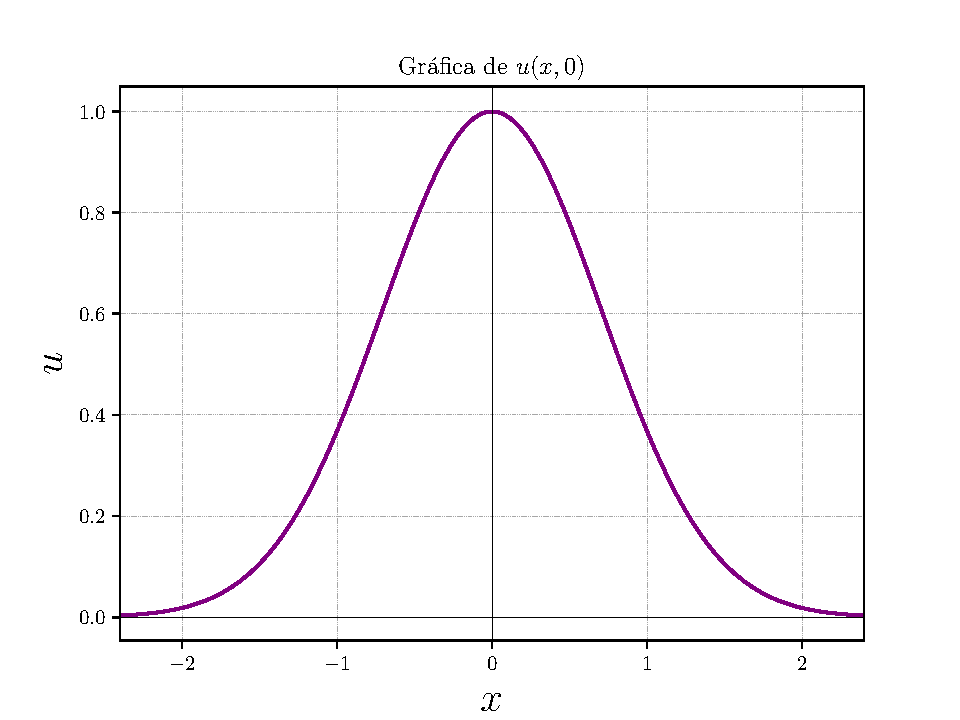
\includegraphics[width=\linewidth]{../some_plots/cond_inicial.pdf}
		\caption{Gráfica de $u(x,0) = \exp(-x^2)$.}
		\label{fig:subfig1}
	\end{subfigure}%
	\begin{subfigure}{0.5\textwidth}
		\centering
		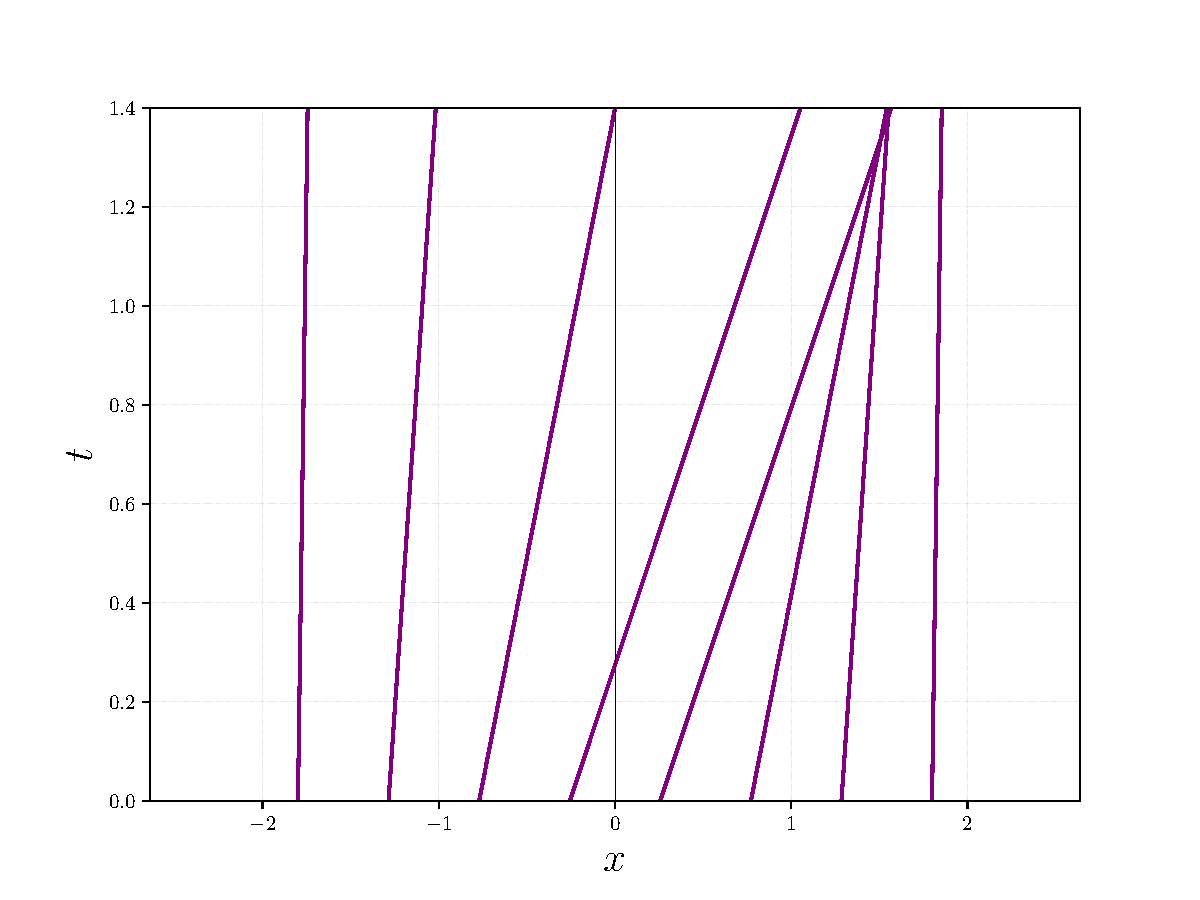
\includegraphics[width=\linewidth]{../some_plots/caracteristicas_burgers.pdf}
		\caption{Características de la ecuación de Burgers.}
		\label{fig:subfig2}
	\end{subfigure}
	\caption{Gráficas de la condición inicial $u(x,0) = \exp(-x^2)$ para la ecuación de Burgers y de algunas características asociadas a esta condición inicial. \textbf{Fuente:} elaboración propia.}
	\label{fig:figura_completa}
\end{figure}
\subsection{Ondas de choque}
Como se puede observar en la figura (\ref{fig:subfig2}), las características asociadas a una condición inicial con forma gaussiana se intersectan. Entonces, si las características se intersectan, la expresión (\ref{eq:sol-burgers-char}) no está bien definida, sino que $u(x,t)$ puede tomar varios valores a la vez, cada uno correspondiente a una característica diferente. En el caso de la ecuación de Burgers, cuando las características se intersectan, la solución se convierte en una ``función'' con tres valores distintos \cite{Leveque}. Esta solución puede tener sentido en algunos contextos, como en el caso del problema de agua superficial \cite{Leveque}. Sin embargo, en la mayoría de casos esta solución no tiene significado físico ya que la variable $u(x,t)$ representa una velocidad y esta debe devolver un solo valor \cite{Leveque}.

La solución con el comportamiento físico correcto cuando las características se intersectan corresponde a una discontinuidad que se propaga con una velocidad determinada \cite{Leveque}. Este efecto se puede demostrar a través del formalismo de la viscosidad disipada. Al obtener la solución de la ecuación de Burgers viscosa (\ref{eq:burgers-vis}), el parámetro $\varepsilon u_{xx}$ evita que la solución presente una discontinuidad, dado que cuando la onda comienza a presentar el choque, la segunda derivada de $u$ crece más rápido que su primera derivada \cite{Leveque}. Así, al efectuar el límite de $\varepsilon \rightarrow 0$ se puede obtener una discontinuidad absoluta que corresponde a la solución de la ecuación de Burgers sin viscosidad. La tendencia de adquirir una discontinuidad  de las soluciones con menos viscosidad se puede evidenciar en la figura (\ref{fig:viscosas}).

\begin{figure}[ht]
	\begin{subfigure}{0.5\textwidth}
		\centering
		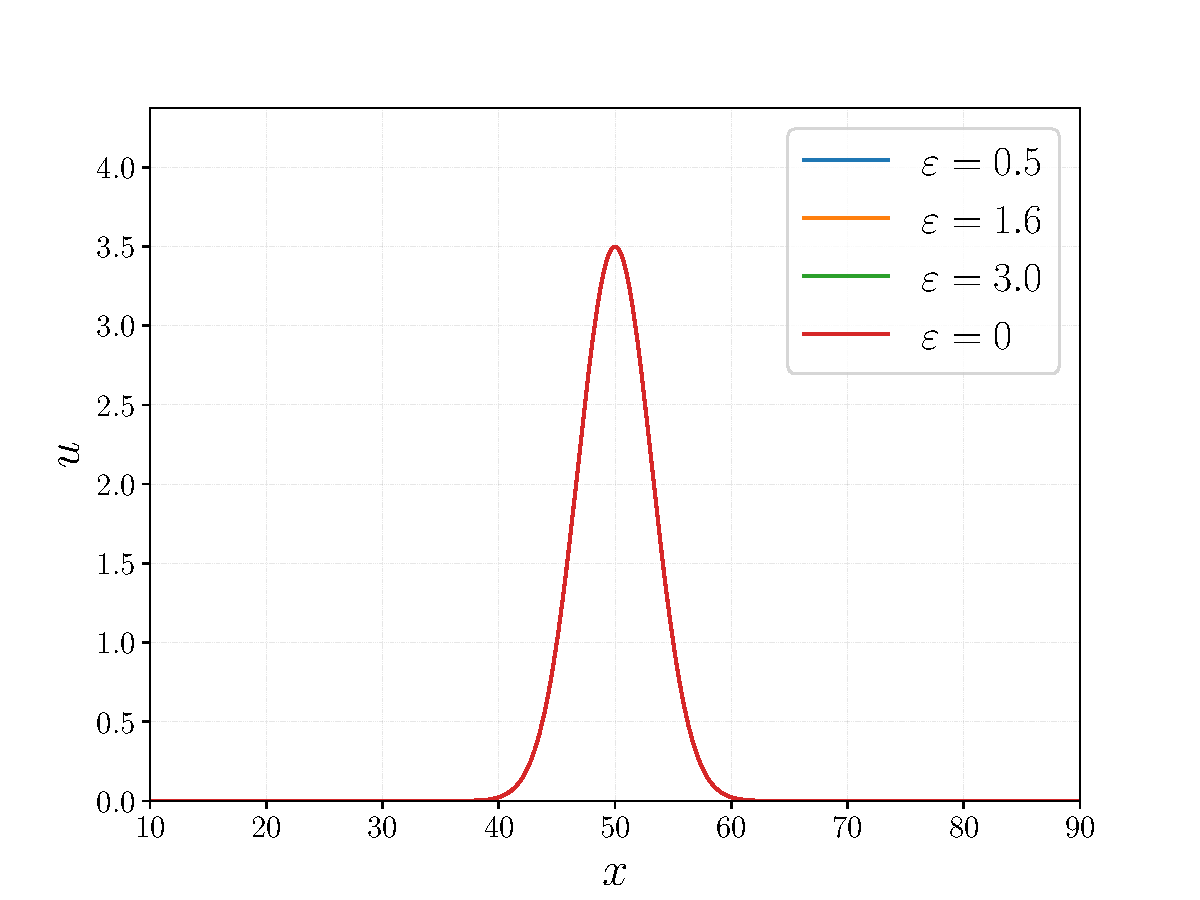
\includegraphics[width=\linewidth]{../some_plots/burgers-viscosas/graficas/viscosidades-1.pdf}
%		\caption{.}
		\label{fig:viscosas1}
	\end{subfigure}%
	\begin{subfigure}{0.5\textwidth}
		\centering
		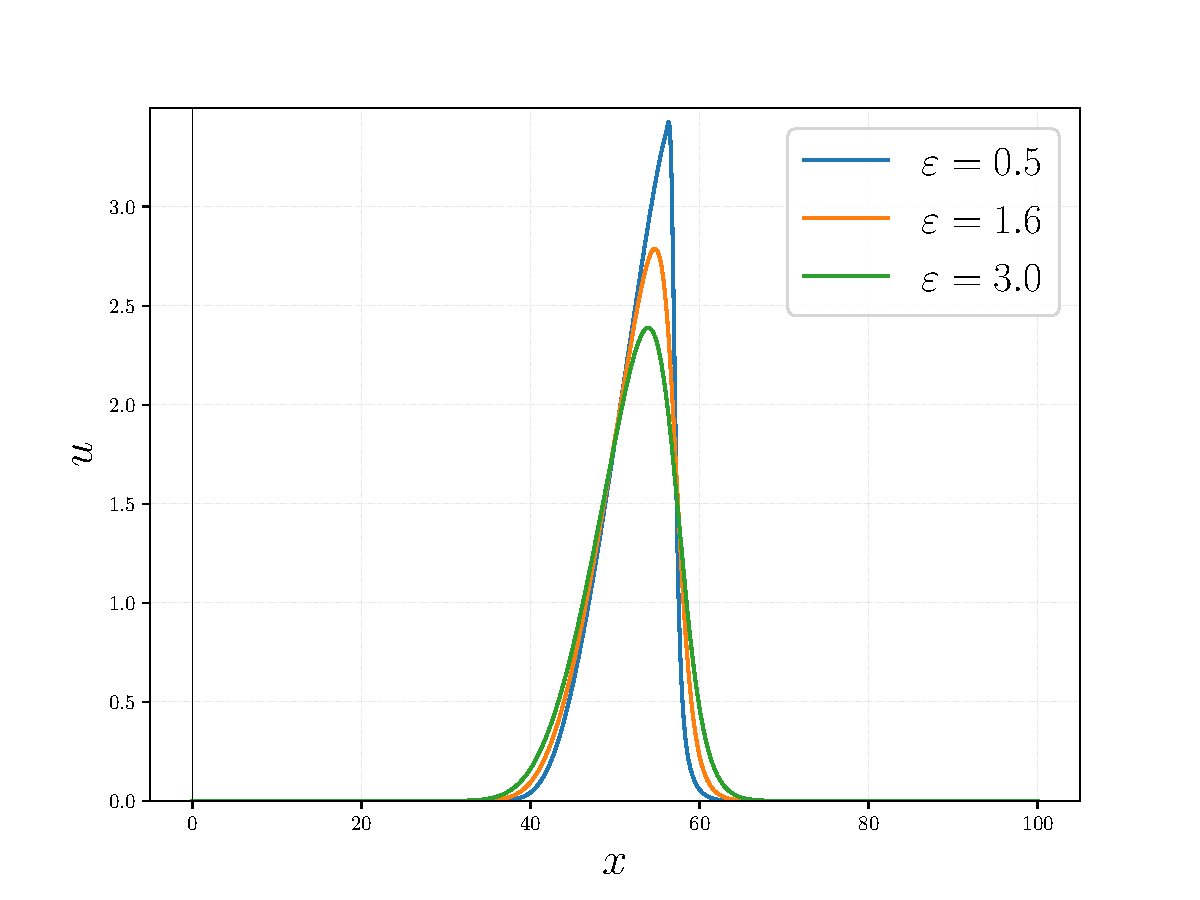
\includegraphics[width=\linewidth]{../some_plots/burgers-viscosas/graficas/viscosidades-100.pdf}
%		\caption{.}
		\label{fig:viscosas2}
	\end{subfigure}
	\begin{subfigure}{0.5\textwidth}
		\centering
		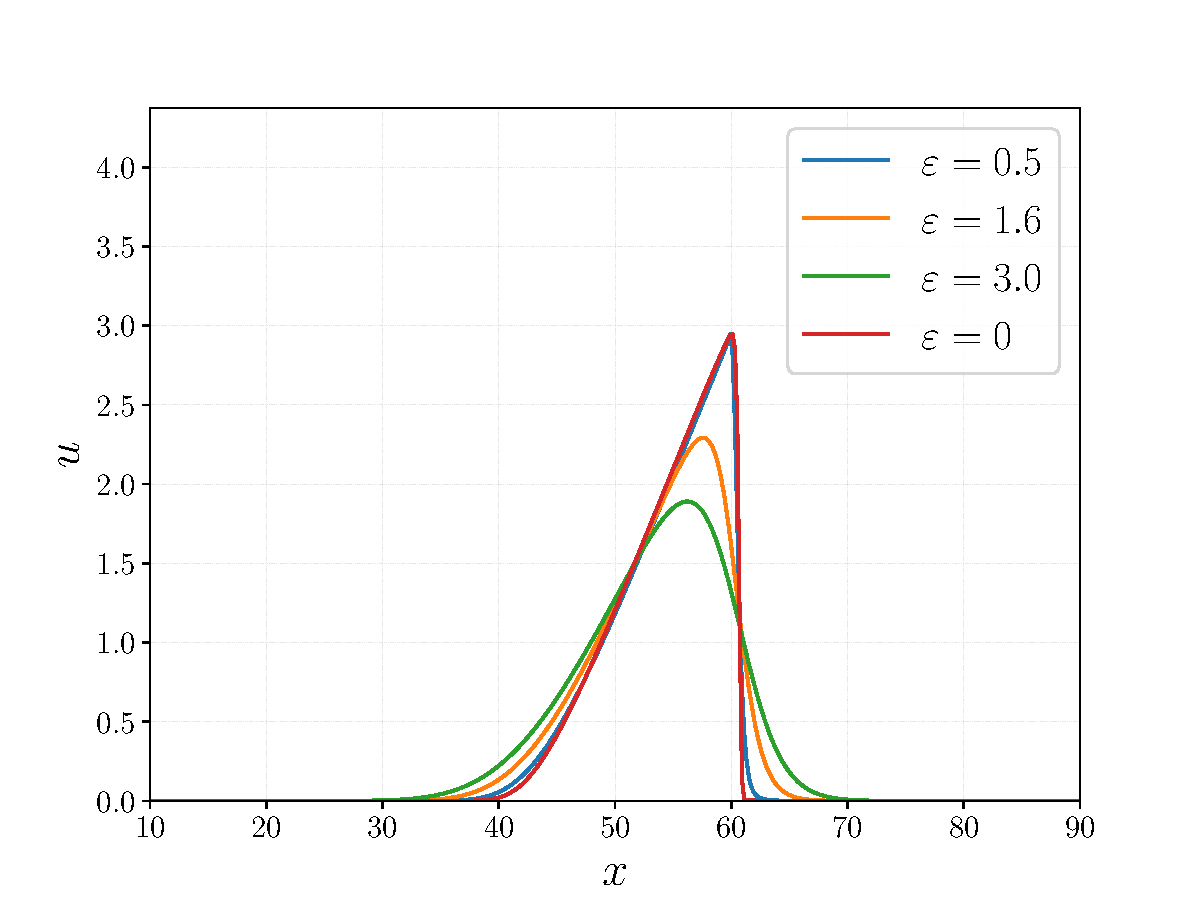
\includegraphics[width=\linewidth]{../some_plots/burgers-viscosas/graficas/viscosidades-200.pdf}
%		\caption{.}
		\label{fig:viscosas3}
	\end{subfigure}
	\begin{subfigure}{0.5\textwidth}
		\centering
		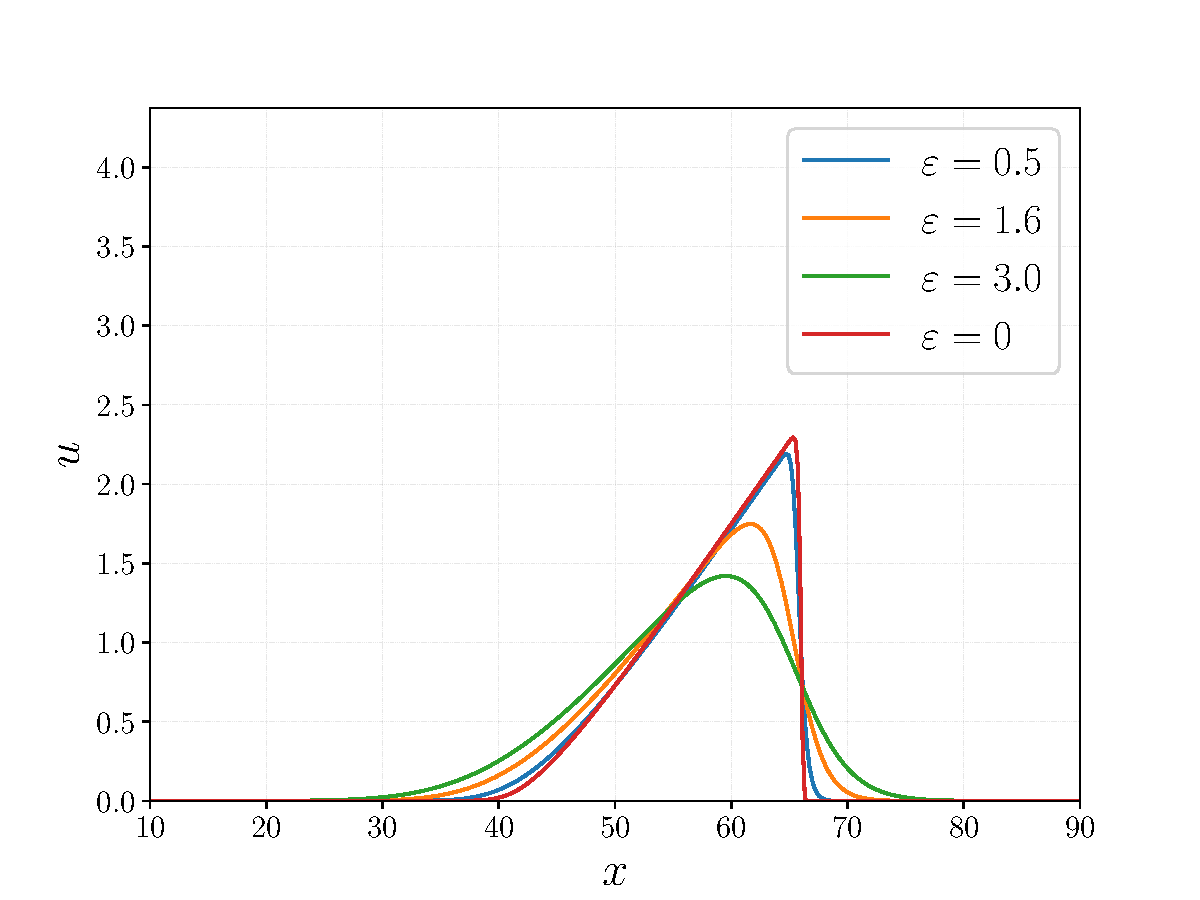
\includegraphics[width=\linewidth]{../some_plots/burgers-viscosas/graficas/viscosidades-400.pdf}
%		\caption{.}
		\label{fig:viscosas4}
	\end{subfigure}
	\caption{Gráficas de las soluciones numéricas, en distintos instantes de tiempo, de la ecuación de Burgers viscosa para distintos valores de coeficiente de viscosidad cinemática ($\varepsilon$), incluyendo el caso donde no hay viscosidad (en rojo). \textbf{Fuente:} elaboración propia.}
	\label{fig:viscosas}
\end{figure}

\section{Problema de Riemann}
Como se ha mostrado, las soluciones a las ecuaciones de conservación admiten soluciones débiles que pueden presentar discontinuidades tanto en la condición inicial como en la evolución temporal de las mismas. Por esta razón, es natural estudiar sistemas hiperbólicos con condiciones iniciales discontinuas, este problema es conocido como \textbf{problema de Riemann}. En el caso escalar, el problema de Riemann para una ecuación de conservación de la forma $u_t + f(u)_x = 0$ corresponde a la siguiente condición inicial
\begin{equation}
	u(x,0) = 
	\begin{cases}
		u_L & \text{si } x < 0 \\
		u_R & \text{si } x \geq 0,
		\label{eq:riemannLR}
	\end{cases}
\end{equation}
en donde la solución es determinada por la relación entre $u_L$ y $u_R$ \cite{Leveque}.
\subsection{Solución al problema de Riemann para la ecuación de Burgers}
Para encontrar la solución al problema de Riemann de la ecuación de Burgers es necesario considerar dos casos.
\subsubsection{Caso $u_L > u_R$:}
La función
\begin{equation}
	u(x,t) = 
	\begin{cases}
		u_L, & \hspace{3mm} x < st \\
		u_R, & \hspace{3mm} x > st,		
	\end{cases}\label{eq:solriemannLR}
\end{equation}
conocida como \textbf{onda de choque}, representa una discontinuidad trasladándose a través del eje $x$ con una velocidad $s$. Esta última es una solución débil de la ecuación de Burgers, para la condición inicial (\ref{eq:riemannLR}), si se cumple la condición general de  \textbf{Rankine - Hugoniot} \cite{Cameron}, que se define como:
\begin{equation}
	f(u_L) - f(u_R) = s(u_L - u_R),
	\label{eq:rankinehugo}
\end{equation}
donde $f(u) = \frac{1}{2} u^{2}$ \cite{Leveque}. A continuación se demuestra la expresión general de la condición Rankine - Hugoniot.\\

\textit{Prueba:} Sea $u$ una solución débil de la ecuación diferencial $u_t + f(u)_x = 0$, de la forma (\ref{eq:solriemannLR}). Sea $\mathcal{M} \gg st$. Aplicando la expresión (\ref{eq:continuidad-1-integral}) a $u$:
\begin{equation}
	\dv{t} \int_{-\mathcal{M}}^{\mathcal{M}}u(x,t)\dd{x} = f(u_L) - f(u_R).
	\label{eq:flux_diff}
\end{equation}
Integrando $u$ a partir de su definición (\ref{eq:solriemannLR}), se tiene
\begin{equation}
	\int_{-\mathcal{M}}^{\mathcal{M}}u(x,t)\dd{x} = (\mathcal{M} + st)u_L + (\mathcal{M} - st)u_R.
\end{equation}
Entonces, sustituyendo en (\ref{eq:flux_diff}),
\begin{equation}
	\dv{t}\left[(\mathcal{M} + st)u_L + (\mathcal{M} - st)u_R\right] = f(u_L) - f(u_R)
\end{equation}
\begin{equation}
	s(u_L - u_R) = f(u_L) - f(u_R),
\end{equation}
se obtiene la condición de salto de Rankine - Hugoniot \cite{Leveque}.

Por lo tanto, para el caso $u_L > u_R$, la solución de la ecuación de Burgers es una discontinuidad que se propaga con una velocidad constante $s = \frac{u_L + u_R}{2}$ \cite{Cameron}.

\begin{figure}[ht]
	\centering
	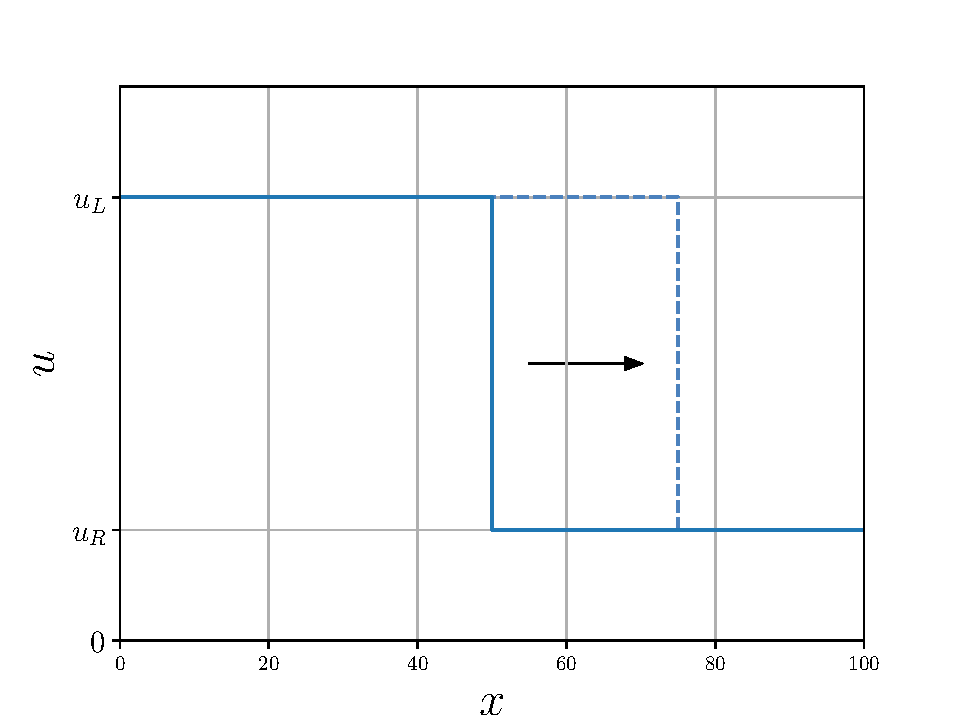
\includegraphics[width=0.8\linewidth]{../some_plots/cap1/graficas/riemannLR.pdf}
	\caption{Ejemplo gráfico de la solución de la ecuación de Burgers para el caso $u_L > u_R$. \textbf{Fuente: }elaboración propia, basada en el esquema obtenido de \cite{Leveque}.}
	\label{fig:solriemannLR}
\end{figure}

\subsubsection{Caso $u_L < u_R$:}
Hay múltiples soluciones débiles para este caso, por ejemplo, la solución (\ref{eq:solriemannLR}) \cite{Cameron} \cite{Leveque}. Sin embargo, esta no es la solución que corresponde a la solución con viscosidad disipiada \cite{Cameron}. La solución
\begin{equation}
	u(x,t) = 
	\begin{cases}
		u_L, & \hspace{3mm} x < u_{L}t \\
		x/t, & \hspace{3mm} u_{L}t \leq x \leq u_{R}t \\
		u_R, & \hspace{3mm} x > u_{R}t,		
	\end{cases}\label{eq:solriemannRL}
\end{equation}
es la solución correspondiente a la viscosidad disipada y es conocida como \textbf{onda de rarefacción} \cite{Leveque}. Resulta ser poco práctico tener que recurrir frecuentemente a la solución de viscosidad disipada para encontrar la solución a cualquier caso del problema de Riemann, por lo que en su lugar se suelen imponer condiciones conocidas como \textbf{condiciones de entropía} que son equivalentes a exigir que la solución sea consistente con el formalismo de viscosidad disipada \cite{Leveque}.

\begin{figure}[ht]
	\begin{subfigure}{0.5\textwidth}
		\centering
		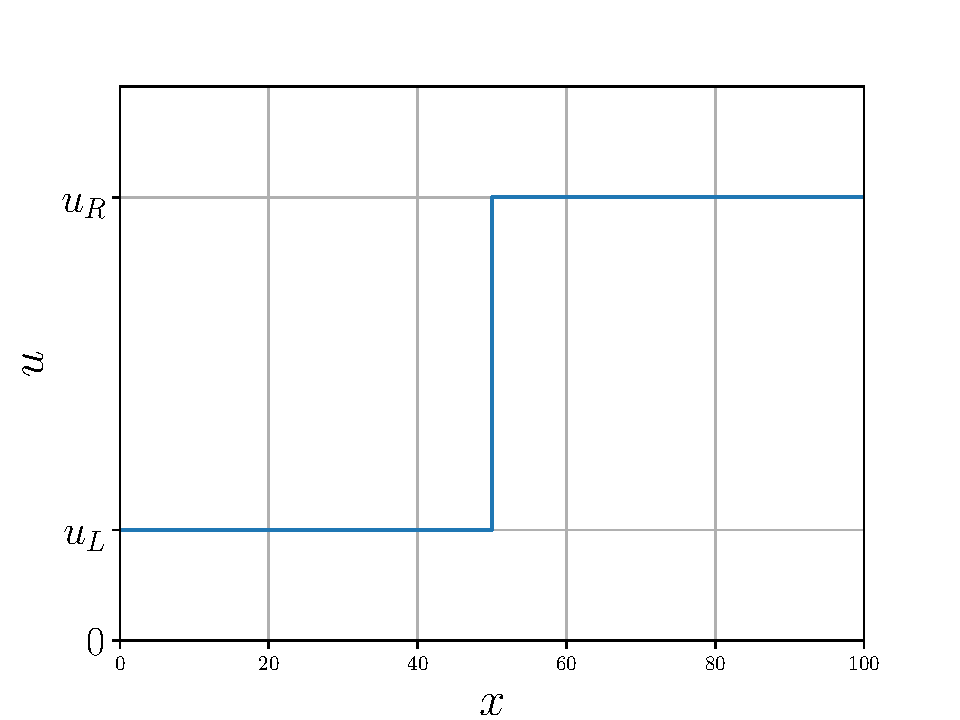
\includegraphics[width=\linewidth]{../some_plots/cap1/graficas/riemannRL-0.pdf}
		%		\caption{.}
%		\label{fig:rarefaccion}
	\end{subfigure}%
	\begin{subfigure}{0.5\textwidth}
		\centering
		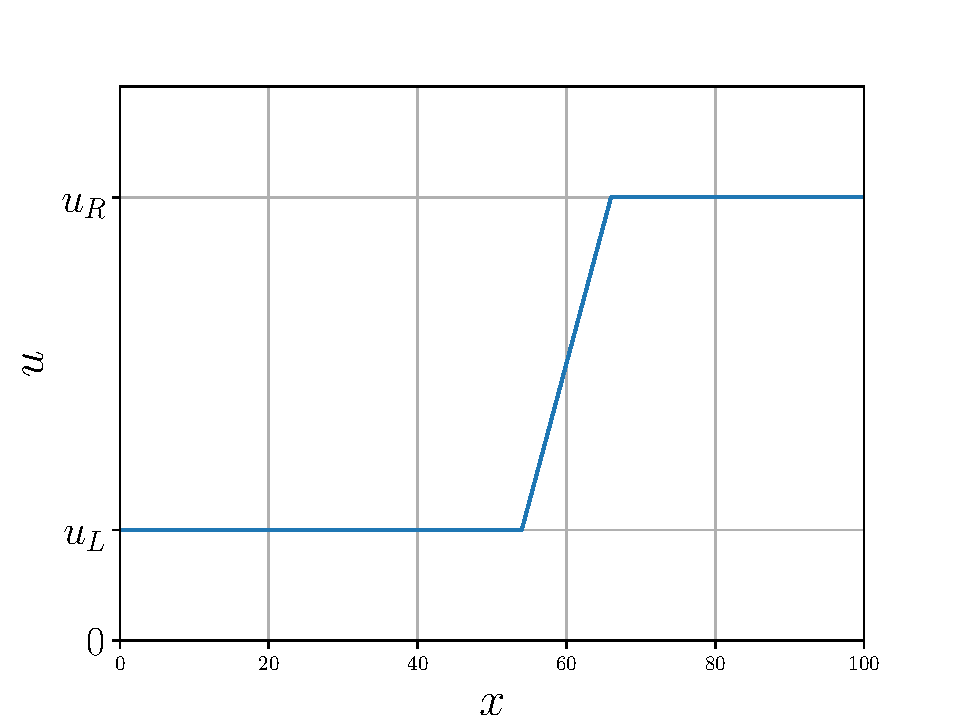
\includegraphics[width=\linewidth]{../some_plots/cap1/graficas/riemannRL-0.4.pdf}
		%		\caption{.}
%		\label{fig:viscosas2}
	\end{subfigure}
	\begin{subfigure}{0.5\textwidth}
		\centering
		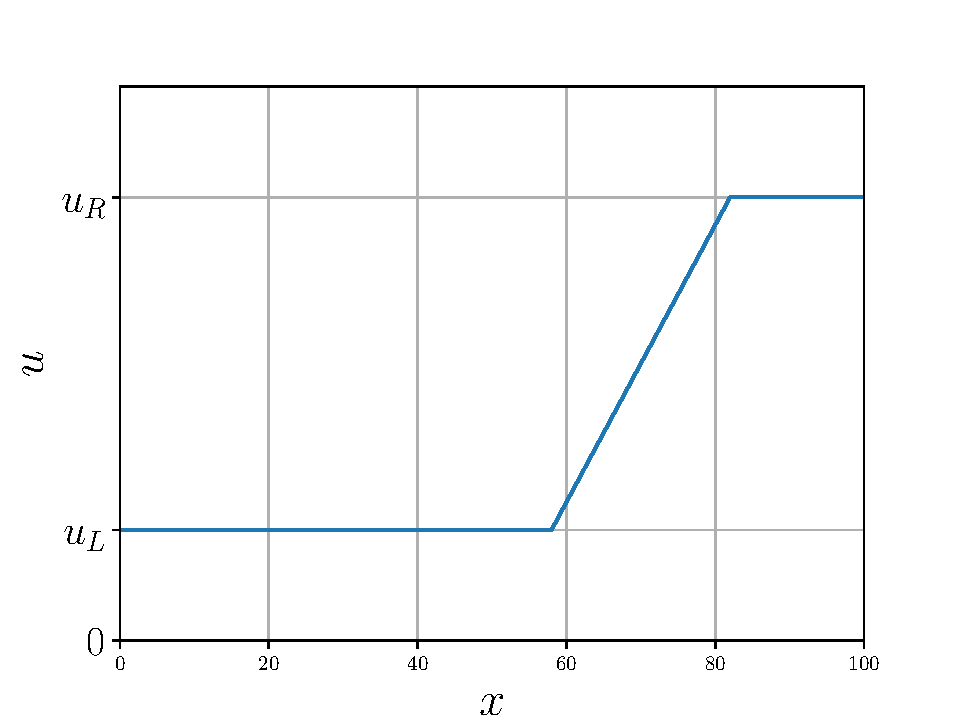
\includegraphics[width=\linewidth]{../some_plots/cap1/graficas/riemannRL-0.8.pdf}
		%		\caption{.}
%		\label{fig:viscosas3}
	\end{subfigure}
	\begin{subfigure}{0.5\textwidth}
		\centering
		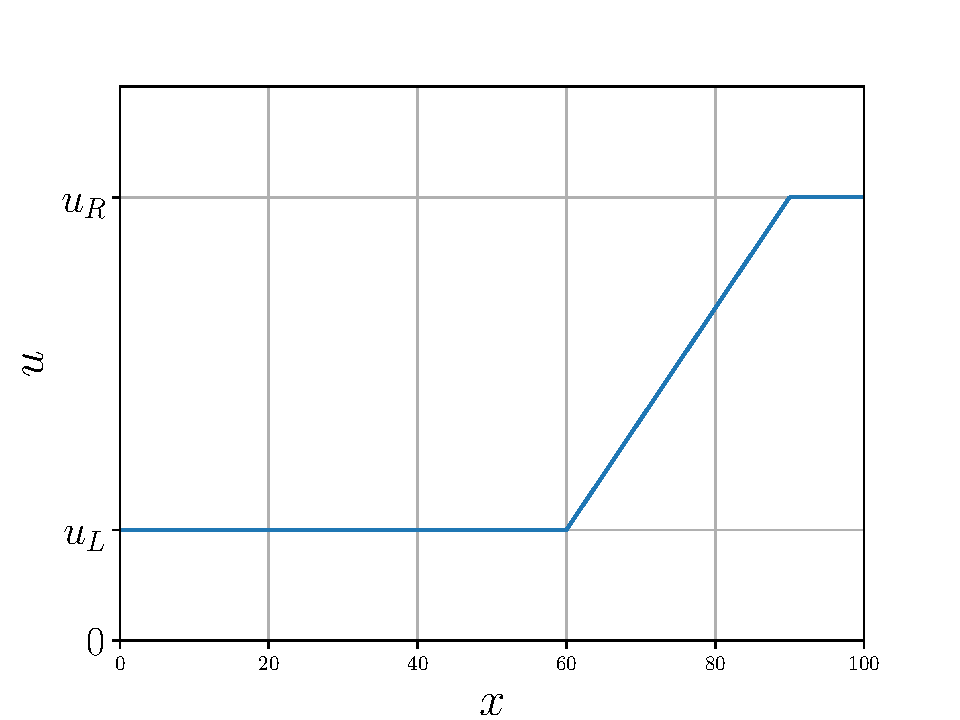
\includegraphics[width=\linewidth]{../some_plots/cap1/graficas/riemannRL-1.pdf}
		%		\caption{.}
%		\label{fig:viscosas4}
	\end{subfigure}
	\caption{Gráficas de las soluciones, en distintos instantes de tiempo, de la ecuación de Burgers para el caso $u_L < u_R$ del problema de Riemann \textbf{Fuente:} elaboración propia.}
	\label{fig:rarefaccion}
\end{figure}
      % Cap. 1 

\chapter{MÉTODO DE VOLÚMENES FINITOS Y ESQUEMA DE ROE}
A continuación se describen el método y los esquemas a utilizar para llevar a cabo una solución numérica de una ecuación de conservación. La idea principal del capítulo es describir el método de volúmenes finitos y la motivación de su uso. Se explicarán los esquemas adecuados para aplicar el mencionado método, un solucionador del problema de Riemann, denominado esquema de Godunov y otro solucionador aproximado del problema de Riemann, denominado esquema de Roe. Este último es el esquema elegido para resolver las ecuaciones de Euler en este texto.\\
El contenido de este capítulo se basa en la parte \textit{Numerical Methods} del texto \cite{Leveque} de Randall LeVeque.

\section{Método de volúmenes finitos}
El método de volúmenes finitos (MVF) es un método numérico de integración que se especializa en resolver ecuaciones diferenciales escritas en forma conservativa. El MVF destaca por ofrecer una interpretación peculiar de la función a resolver, ya que es un método basado en la forma \textbf{integral} de las ecuaciones.

Sea $D = [a,b]$ el dominio espacial de una ecuación de conservación.





%Se describe la estructura del método de volúmenes finitos, principalmente para resolver ecuaciones de conservación y se enfatiza su importancia al aplicarse a problemas de esta naturaleza. Se introducen los conceptos de discretización, ecuación de diferencias, esquema numérico, celda. Se comenta sobre las condiciones de estabilidad de una solución numérica.
%
%Se exponen algunos esquemas numéricos generales aproximados. Se introduce el esquema de Roe y su relación con el problema de Riemann. Nuevamente, se utiliza como ejemplo la ecuación de Burgers para proporcionar una idea simple de la aplicación de estos esquemas.      % Cap. 2 

\chapter{ECUACIONES DE EULER Y APLICACIÓN DEL ESQUEMA DE ROE}

En este capítulo se explican y derivan las ecuaciones de Euler utilizando las variables generales (presión, densidad y velocidad) y se introducen las variables conservadas. Se explican las ligaduras adicionales involucradas para que las ecuaciones de Euler sean aplicadas a un gas ideal poliatómico.

Se describe el esquema de Roe implementado en la solución de las ecuaciones de Euler para un gas ideal poliatómico así como las demás especificaciones requeridas por el método de volúmenes finitos. Se explica la implementación del método numérico en \texttt{C++}. Se muestran los resultados obtenidos para un problema de condiciones iniciales específicas.
\section{Ecuaciones de Euler}
Las ecuaciones fundamentales de la dinámica de fluidos se basan en las siguientes leyes de conservación universales:
\begin{itemize}
	\item Conservación de la masa
	\item Conservación del momentum
	\item Conservación de la energía.
\end{itemize}
La ecuación de conservación de la masa, que se derivó en la sección (\ref{sec:derivacion-continuidad}), consiste en aplicar la ecuación de continuidad para un fluido con cierta densidad. La ley de conservación del momentum resulta al aplicar la Segunda Ley de Newton en un fluido. Por último, la ley de conservación de la energía es equivalente a la aplicación de la Primera Ley de la Termodinámica. Además de las tres ecuaciones de conservación, es necesario establecer una relación entre las variables físicas del fluido, de tal manera que el sistema de ecuaciones sea resoluble \cite{heattransfer}. En el caso de un gas ideal, la ecuación adicional que relaciona las variables densidad $\rho$, presión $p$ y temperatura $T$, es la ecuación de estado. 
\subsection{Derivación de las ecuaciones}
%\subsubsection{Ecuación de continuidad}
La ecuación de continuidad, derivada en la sección (\ref{sec:derivacion-continuidad}) tiene la siguiente forma
\begin{equation}
	\rho_{t} + (\rho v)_{x} = 0.
	\label{eq:continuidad-euler}
\end{equation}
Ya que el flujo asociado a esta ecuación de conservación es $\rho v$, se puede interpretar que, generalmente, para cualquier cantidad física $z$ que sufra advección, su flujo estará dado por el producto de la cantidad por la velocidad de advección, i.e., $f=zv$. 

A partir del último razonamiento, el flujo asociado a la advección de momentum $\rho v$, tiene una contribución al flujo dada por $(\rho v) \cdot v = \rho v^2$. Sin embargo, además de la advección que sufre el momentum, deben considerarse las fuerzas que actúan en el fluido para expresar el flujo total del momentum. En este texto no se considerarán fuerzas externas, por lo que únicamente habría que tomar en cuenta la fuerza interna del fluido, que está dada por el gradiente de \textbf{presión}, $p_x$ \cite{LeVeque}. De esta manera, se consigue la ecuación de conservación del momentum:
\begin{equation}
	(\rho v)_t + (\rho v^{2} + p)_{x} = 0.
	\label{eq:momentum-euler}
\end{equation}

Para derivar la conservación de energía, se debe considerar que ésta se compone por un término cinético y uno correspondiente a la energía interna del fluido. Sea $E$ la densidad de energía total de un fluido. Entonces, se tiene que:
\begin{equation}
	E = \frac{1}{2} v^{2} + e,
	\label{eq:energia}
\end{equation}
donde el término $\frac{1}{2} v^{2}$ corresponde a la densidad de energía cinética por unidad de masa y $e$ es la \textbf{energía interna} por unidad de masa del fluido, que también suele denominarse como energía interna específica. La energía interna depende de los grados de libertad internos de las moléculas de los gases, considerando energía de rotación, cinética, de vibración y otras formas más complejos de energía. Las ecuaciones de Euler asumen que el fluido se encuentra en equilibrio termodinámico y que la ecuación de estado provee una expresión para la energía interna específica tal que ésta depende de la presión y la densidad del fluido únicamente
\begin{equation}
	e = e(p, \rho).
\end{equation}
De igual manera que con el momentum, la energía total se ve afectada por la advección del flujo del fluido. Dado que no se consideran fuerzas externas que afecten al sistema, únicamente la presión del fluido hace trabajo y es proporcional al gradiente de $vp$. Entonces la ecuación de conservación de la energía se reduce a:
\begin{equation}
	(\rho E)_{t} + [v(\rho E + p)]_{x} = 0.
	\label{eq:energia-euler}
\end{equation}
haciendo notar que $\rho E$ corresponde a la energía total del gas.

Las ecuaciones de Euler, (\ref{eq:continuidad-euler}), (\ref{eq:momentum-euler}) y (\ref{eq:energia-euler}) se pueden escribir en forma vectorial, obteniendo:
\begin{equation}
	\begin{bmatrix}
		\rho \\
		\rho v \\
		\rho E
	\end{bmatrix}_{t}
+
	\begin{bmatrix}
		\rho v \\
		\rho v^{2}+p \\
		v(\rho E + p)
	\end{bmatrix}_{x}
= 0,
\label{eq:euler-eqs-1}
\end{equation}
cuya forma coincide con la presentada en (\ref{eq:conservacion}). Cabe mencionar que en este texto se considerarán problemas unidimensionales solamente.

%Para escribir el sistema (\ref{eq:euler-eqs-1}) de la forma (\ref{eq:conservacion-jacobiana}) 

\subsection{Ecuación de estado para un gas politrópico}
Para completar el sistema de ecuaciones de Euler, es necesario definir la ecuación de estado que relacione la energía con las variables físicas de presión y  densidad. El desarrollo de la ecuación de estado para un gas ideal sigue de cerca la sección \textit{Ideal Gas} del capítulo \textit{Some Linear Systems} en \cite{LeVeque}.

La energía interna de un gas idea es únicamente dependiente de la temperatura,
\begin{equation}
	e = e(T).
\end{equation}
Mientras que la temperatura se relaciona con la presión y densidad a través de la ley del gas ideal, que define al mismo. Esta es:
\begin{equation}
	p = \mathcal{R}\rho T
	\label{eq:ideal-gas-law}
\end{equation}
donde $\mathcal{R}$ es la constante específica de los gases, que se define como el cociente entre la constante de Boltzmann $k_B$ y  la masa de cada molécula del gas $m$ \cite{blundell}. Por otro lado, la energía interna específica es proporcional a la temperatura,
\begin{equation}
	e = c_{v}T
	\label{eq:energia-interna-1}
\end{equation}
donde $c_{v}$ es la capacidad calorífica específica a volumen constante. Los gases que cumplen con esta propiedad se conocen como gases \textbf{politrópicos}. Entonces, si se cambiase la temperatura de un gas en una cantidad infinitesimal $\dd{T}$, manteniendo el volumen constante, se obtendría
\begin{equation}
	\dd{e} = c_{v} \dd{T}
\end{equation}
como cambio infinitesimal de energía interna específica. En cambio, si se permite que el gas se expanda pero manteniendo ahora la presión constante, se obtendría una expresión para el cambio de energía considerando al trabajo, $W = -p\dd{V}$, realizado sobre el gas, esto es
\begin{equation}
	m\dd{e} = \dd{W} + \dbar Q
\end{equation}
\begin{equation}
	m\dd{e} = -p\dd{V} + \dbar Q
\end{equation}
\begin{equation}
	\dd{e} = -\frac{p}{m}\dd{V} + c_{p}\dd{T}
\end{equation}
y puesto que al usar $\rho = \frac{m}{V}$, se obtiene que $\dd{V} = m\dd(\frac{1}{\rho})$, entonces:
\begin{equation}
	\dd{e} = -p\dd(\frac{1}{\rho}) + c_{p}\dd{T}
\end{equation}
\begin{equation}
	\dd(e + \frac{p}{\rho}) = c_{p}\dd{T},
	\label{eq:entalpia-temp-dif}
\end{equation}
donde $c_p$ es la capacidad calorífica específica del gas a presión constante. A partir del anterior resultado se define la \textbf{entalpía} interna $\mathrm{h}_i$:
\begin{equation}
	\mathrm{h}_i \equiv e + \frac{p}{\rho},
	\label{eq:entalpia-1}
\end{equation}
mientras que la entalpía total $\mathrm{h}$ \footnote{No confundir con $h$ definida en \ref{eq:def-h} como el tamaño de cada celda del dominio.} es:
\begin{equation}
	\mathrm{h} = E + \frac{p}{\rho}.
	\label{eq:entalpia-total}
\end{equation}
Para un gas politrópico se considera a $c_p$ como constante, por lo que integrando la ecuación (\ref{eq:entalpia-temp-dif}) se obtiene otra expresión para la entalpía interna,
\begin{equation}
	\mathrm{h}_i = c_p T.
	\label{eq:entalpia-2}
\end{equation}
Por otro lado, de acuerdo a la ley del gas ideal, se tiene la siguiente relación
\begin{equation}
	c_p - c_v = \mathcal{R}.
	\label{eq:diferencia-capacidades}
\end{equation}
Para continuar con la derivación, es conveniente definir el \textbf{coeficiente de dilatación adiabática} $\gamma$ como:
\begin{equation}
	\gamma \equiv \frac{c_p}{c_v}.
	\label{eq:gamma-1}
\end{equation}
Dicha cantidad está estrechamente relacionada con el número de grados de libertad internos del gas, que depende de la naturaleza del mismo. Según el teorema de equipartición de la energía, el promedio de energía involucrada en cada grado de libertad es el mismo. Específicamente, cada grado de libertad aporta una cantidad promedio de energía por molécula de $\frac{1}{2}k_B T$. De tal manera que si existen ${\alpha}$ grados de libertad internos en un gas que tiene $n$ moléculas por unidad de masa, se obtiene una expresión para la energía interna específica
\begin{equation}
	e = \frac{\alpha}{2}n k_B T
\end{equation}
o bien, 
\begin{equation}
	e = \frac{\alpha}{2}\mathcal{R} T.
	\label{eq:energia-interna-2}
\end{equation}
Comparando con (\ref{eq:energia-interna-1}) se obtiene
\begin{equation}
	c_v = \frac{\alpha}{2}\mathcal{R},
\end{equation}
sustituyendo en (\ref{eq:diferencia-capacidades}),
\begin{equation}
	c_p = \left(1+\frac{\alpha}{2}\right)\mathcal{R}.
\end{equation}
Y al aplicar la definición de $\gamma$ en (\ref{eq:gamma-1}) se obtiene la expresión
\begin{equation}
	\gamma = \frac{\alpha + 2}{\alpha},
\end{equation}
que, como se expuso previamente, relaciona el número de grados de libertad con el coeficiente de dilatación adiabática. Por ejemplo, para gases monoatómicos se consideran únicamente tres grados de libertad, correspondientes al movimiento traslacional en tres dimensiones, por lo que $\alpha = 3$ y $\gamma = 5/3$. En gases diatómicos (como el aire, compuesto por $H_2$ y $N_2$ principalmente) se agregan dos grados libertad correspondientes a dos ejes de rotación posibles para cada molécula, de tal manera que $\alpha = 5$ y $\gamma = 7/5 = 1.4$.

Por último, se escribe la ecuación de estado del gas ideal para la energía utilizando  (\ref{eq:ideal-gas-law}),
\begin{equation}
	e = c_v T = \frac{c_v}{\mathcal{R}}\cdot\frac{p}{\rho}
\end{equation}
\begin{equation}
	e = \frac{p}{(\gamma - 1) \rho}.
\end{equation}
De tal manera que la energía total del gas ($\rho E$) queda como
\begin{equation}
	 \rho E = \frac{1}{2}\rho v^{2} + \frac{p}{\gamma - 1}.
	 \label{eq:energia-total}
\end{equation}
\section{Aplicación del esquema de Roe}
Para aplicar el esquema de Roe en la expresión del método de volúmenes finitos, dada por 
\begin{equation}
	U_{i}^{n+1}-U_{i}^{n} = 
	\frac{k}{h}\left[ F(U_{i-1}^n, U_i^n) - F(U_{i}^n, U_{i+1}^n) \right],
	\label{eq:metodo-vol-finitos-3}
\end{equation}
 es necesario definir el flujo entre cada interfaz, $F_{i\pm \frac{1}{2}}$. La expresión de dicho flujo, en su forma simple, se detalló en (\ref{eq:roe-flux}). Mientras que la versión del flujo en conjunto con la corrección de entropía es (\ref{eq:flux-HH-fix}). Por tanto, el siguiente paso es construir el flujo de Roe de acuerdo a las aproximaciones correspondientes.
\subsection{Variables conservadas y propiedades de $\mathbf{A(\mathbf{U})}$}
Para implementar el método de volúmenes finitos junto al esquema de Roe en la solución numérica de las ecuaciones de Euler es necesario identificar las \textbf{variables conservadas} involucradas en la definición de un sistema general de conservación, definido en (\ref{eq:conserv-deriv-short}). Comparando esta expresión con el sistema (\ref{eq:euler-eqs-1}) se obtiene:
\begin{equation}
	\mathbf{U} = 
	\begin{bmatrix}
		\mathbf{u}_1 \\
		\mathbf{u}_2 \\
		\mathbf{u}_3
	\end{bmatrix} \equiv
	\begin{bmatrix}
		\rho \\
		\rho v \\
		\rho E
	\end{bmatrix}
\end{equation}
\begin{equation}
	\mathbf{F} = 
	\begin{bmatrix}
		\mathbf{f}_1 \\
		\mathbf{f}_2 \\
		\mathbf{f}_3
	\end{bmatrix} \equiv
	\begin{bmatrix}
		\rho v \\
		\rho v^2 + p \\
		v(\rho E + p)
	\end{bmatrix}.
\label{eq:flujo-euler-exacto}
\end{equation}
Por tanto, se define a $\mathbf{u}_i$ como la i-ésima variable conservada cuyo  flujo correspondiente es $\mathbf{f}_i$. 

Por otro lado, el esquema de Roe depende de los autovalores y autovectores de la matriz jacobiana $\mathbf{A(\mathbf{U})}$ definida en (\ref{eq:conservacion-jacobiana}). Aplicando la definición (\ref{eq:jacobiana-A-definicion}) mientras se toma en cuenta la ecuación de estado para la energía (\ref{eq:ideal-gas-law}), se obtiene una expresión para esta matriz:
\begin{equation}
	\mathbf{A(\mathbf{U})} =
	\begin{bmatrix}
		0 & 1 & 0 \\
		\frac{1}{2}(\gamma - 3)v^2 & (3  - \gamma) v & (\gamma - 1) \\
		\frac{1}{2}(\gamma - 1)v^3 - v(\rho E+p)/\rho & (\rho E+p)/\rho-(\gamma - 1)v^2 & \gamma v \\
	\end{bmatrix}.
\end{equation}
Seguidamente, se deben calcular los autovalores y autovectores de esta matriz. Siguiendo la notación de los últimos capítulos, al autovalor $\lambda_i$ le corresponde el autovector $\mathbf{r}_i$, y estos son:
\begin{equation}
	\lambda_1 = v-c, \hspace{4mm}
	\lambda_2 = c, \hspace{4mm}
	\lambda_3 = v+c,
\end{equation}
\begin{equation}
	\mathbf{r}_1 = 
	\begin{bmatrix}
		1 \\
		v-c \\
		\mathrm{h}-vc
	\end{bmatrix},\hspace{4mm}
	\mathbf{r}_2 = 
	\begin{bmatrix}
		1 \\
		v \\
		\frac{1}{2}v^{2}
	\end{bmatrix},\hspace{4mm}
	\mathbf{r}_3 = 
	\begin{bmatrix}
		1 \\
		v+c \\
		\mathrm{h}+vc
	\end{bmatrix}.
\end{equation}
donde $c$ es la velocidad del sonido, dada por:
\begin{equation}
	c = \sqrt{\frac{\gamma p}{\rho}},
\end{equation}
mientras $\mathrm{h}$ es la entalpía total definida en (\ref{eq:entalpia-total}), o bien, equivalentemente:
\begin{equation}
	\mathrm{h} = \frac{1}{2}v^2 + \left(\frac{\gamma}{\gamma - 1}\right)\frac{p}{\rho}.
\end{equation}
Por lo tanto, es posible escribir la velocidad del sonido en términos de la entalpía y la velocidad:
\begin{equation}
	c^2 = (\gamma - 1)\left[\mathrm{h} - \tfrac{1}{2}v^{2}\right].
\end{equation}
\subsection{Valores promediados de Roe}
Retornando a la expresión para el flujo numérico simple de Roe,
\begin{equation}
	F(\mathbf{U}_L, \mathbf{U}_R) = \frac{1}{2}\left(\mathbf{F}(\mathbf{U}_L) +\mathbf{F}(\mathbf{U}_R)\right) - 
	\frac{1}{2}\sum_{p=1}^{m}|\hat{\lambda}_{p}|\alpha_{p}\mathbf{\hat{r}}_{p},
	\label{eq:roe-flux-2}
\end{equation}
se destaca que es necesario encontrar los autovalores $\hat{\lambda}_i$ y autovectores $\hat{r}_i$ correspondientes a la matriz aproximada $\mathbf{\hat{A}}$. Roe \cite{roe81} propuso expresiones, basadas en promedios específicos de los valores adyacentes, para los mencionados autovectores y autovalores de la matriz aproximada y junto a Pike demostraron que son los únicos promedios que satisfacen las condiciones necesarias impuestas al flujo numérico del esquema de Roe \cite{roe86}. Los autovalores y autovectores de Roe son:
\begin{equation}
	\hat{\lambda}_1 = \tilde{v}-\tilde{c}, \hspace{4mm}
	\hat{\lambda}_2 = \tilde{c}, \hspace{4mm}
	\hat{\lambda}_3 = \tilde{v}+\tilde{c},
\end{equation}
\begin{equation}
	\mathbf{\hat{r}}_1 = 
	\begin{bmatrix}
		1 \\
		\tilde{v}-\tilde{c} \\
		\tilde{\mathrm{h}}-\tilde{v}\tilde{c}
	\end{bmatrix},\hspace{4mm}
	\mathbf{\hat{r}}_2 = 
	\begin{bmatrix}
		1 \\
		\tilde{v} \\
		\frac{1}{2}\tilde{v}^{2}
	\end{bmatrix},\hspace{4mm}
	\mathbf{\hat{r}}_3 = 
	\begin{bmatrix}
		1 \\
		\tilde{v}+\tilde{c} \\
		\tilde{\mathrm{h}}+\tilde{v}\tilde{c}
	\end{bmatrix}.
\end{equation}
 Mientras que los coeficientes de las características $\alpha_{i}$ están dados por:
 \begin{equation}
 	\alpha_1 = \frac{1}{2\tilde{c}^{2}}[\Delta p - \tilde{\rho}\tilde{c}\Delta v], \hspace{4mm}
 	\alpha_2 = \frac{1}{\tilde{c}^{2}}\left[\tilde{c}^{2}\Delta\rho - \Delta p\right], \hspace{4mm}
 	\alpha_3 = \frac{1}{2\tilde{c}^{2}}[\Delta p + \tilde{\rho}\tilde{c}\Delta v],
 \end{equation}
con
\begin{equation}
	\tilde{\rho} = \sqrt{\rho_L \rho_R}
	\label{eq:rho-prom}
\end{equation}
\begin{equation}
	\tilde{v} = \frac{\sqrt{\rho_{L}}\cdot v_L + \sqrt{\rho_{R}}\cdot v_R}{\sqrt{\rho_{L}} + \sqrt{\rho_{R}}}
\end{equation}
\begin{equation}
	\tilde{\mathrm{h}} = \frac{\sqrt{\rho_{L}}\cdot \mathrm{h}_L + \sqrt{\rho_{R}}\cdot \mathrm{h}_R}{\sqrt{\rho_{L}} + \sqrt{\rho_{R}}}
\end{equation}
\begin{equation}
	\tilde{c}^{2} = (\gamma - 1)[\tilde{h} - \tfrac{1}{2}\tilde{v}^2]
	\label{eq:c-prom}
\end{equation}
donde $\Delta u = u_R - u_L$, para cualquier variable $u$, siendo $u_R$ y $u_L$ el valor de la variable a la derecha e izquierda de la interfaz en donde se calcula el flujo, respectivamente.
\section{Características básicas de la simulación}
Para resolver las ecuaciones de Euler es necesario especificar algunas características del medio y  del espacio en el que toman lugar las simulaciones a presentar en este texto. 
\subsection{Dimensiones}
\label{sec:dimensiones}
Las ecuaciones de Euler serán resueltas en una dimensión espacial, que se puede interpretar como la evolución temporal de un gas dentro de un tubo. Naturalmente, un tubo no es exactamente un objeto unidimensional (un objeto unidimensional es una idealización) pero se aproximará como tal para efectuar la simulación. Este dominio posee una longitud de $10\unit{\meter}$, de tal manera que definiendo los parámetros de la sección (\ref{sec:discretizacion-del-dominio}), se tiene:
\begin{equation}
	a = 0 \unit{\meter},
\end{equation}
\begin{equation}
	b = 10 \unit{\meter}.
\end{equation}
Es natural entonces definir una variable para el largo del dominio, $L\equiv b-a$. Mientras que el número de celdas $N$ a utilizar será:
\begin{equation}
	N = 500.
\end{equation}
De tal forma que el tamaño de cada celda está dado por:
\begin{equation}
	h = \frac{10\unit{\meter}}{500} = 0.02 \unit{\meter}.
\end{equation}
El tiempo total por defecto será de $4\unit{\second}$, y se producirá la solución para un número determinado de instantes temporales en total, que generalmente no coincidirá con el número de instantes temporales calculados. Esto se hace para optimizar el tiempo de cómputo. Por esta razón, el tamaño de paso temporal $k$ puede estar sujeto a cambios dependiendo de la simulación, ya que en caso no se cumpla la condición de estabilidad (\ref{eq:cond-estabilidad}) deberán recalibrarse los parámetros temporales.

A excepción de los resultados mostrados en el capítulo \ref{cap:5}, se tomará el coeficiente de dilatación adiabática como el valor aproximado que posee el aire, $\gamma = 1.4$ \cite{LeVeque}.

\subsection{Condiciones iniciales}
Se experimentará con tres distintos conjuntos de condiciones iniciales para las ecuaciones de Euler. 

\subsubsection{Primer conjunto}
\label{sec:gaussiana41}
Este conjunto corresponde a una solución trivial. Las condiciones iniciales de las variables físicas son las siguientes
\begin{align}
	&\rho(x,0) =  \left(1.0+\exp[-(x-\tfrac{L}{2})^{2}]\right)\hspace{1mm}\unit{\kilogram\per\meter^{3}} \\
	&v(x,0) = 1.0 \hspace{1mm}\unit{\meter\per\second} \\
	&p(x,0) = 0.5 \hspace{1mm}\unit{\pascal}
\end{align}
Notando que tanto la velocidad como la presión son constantes, se espera que el perfil gaussiano definido para la densidad se traslade a velocidad constante sobre el eje $x$. Esto se deriva del hecho de que la ecuación de continuidad \eqref{eq:continuidad-euler} se reduce a una ecuación de advección lineal en este caso.

Los siguientes conjuntos de condiciones iniciales corresponden a funciones definidas por partes. Las variables tendrán un valor constante que depende de la mitad del dominio en donde se valúen. Se adoptará la siguiente notación para escribir de manera compacta las condiciones iniciales:
\begin{equation}
	\mathbf{V}(x,0) = 
	\begin{cases}
		\mathbf{V}_{L} & \text{ si } x \leq L/2\\
		\mathbf{V}_{R} & \text{ si } x > L/2,
	\end{cases}
\end{equation}
donde
\begin{equation}
\mathbf{V}(x,t) = 
	\begin{bmatrix}
		\rho \\
		v \\
		P
	\end{bmatrix},
\end{equation}
es el vector de variables físicas independientes.

\subsubsection{Segundo conjunto}
\label{sec:sod_con_entropy148}
Este conjunto de condiciones iniciales se denomina Test de Sod \cite{thesis-euler-godunov}. Consiste en los siguientes valores para las variables físicas independientes \footnote{Se omiten las dimensiones de las variables para mantener la legibilidad del texto, sin embargo, todas las unidades utilizadas corresponden a las del Sistema Internacional.}

\begin{equation}
\mathbf{V}_L = 
	\begin{bmatrix}
		3.0\\
		0.0\\
		3.0
	\end{bmatrix},\hspace{4mm}
\mathbf{V}_R = 
	\begin{bmatrix}
		1.0\\
		0.0\\
		1.0
	\end{bmatrix}.
\end{equation}
En este conjunto de condiciones iniciales se destaca la diferencia de presión en cada mitad del dominio, así como de la densidad, que va de mayor a menor cantidad. La velocidad inicial del gas es nula.

\subsubsection{Tercer conjunto}
\label{sec:leveque_sin_entropy714}
El siguiente conjunto de condiciones iniciales fue propuesto por LeVeque para evaluar el funcionamiento del esquema numérico utilizado cuando se presentan ondas de rarefacción transónica \cite{pelanti}. Es similar al test de Sod, pero con la diferencia que la velocidad inicial del gas no es nula. Los valores iniciales son:
\begin{equation}
	\mathbf{V}_L = 
	\begin{bmatrix}
		3.0\\
		0.9\\
		3.0
	\end{bmatrix},\hspace{4mm}
	\mathbf{V}_R = 
	\begin{bmatrix}
		1.0\\
		0.9\\
		1.0
	\end{bmatrix}.
\end{equation}
\subsection{Condiciones de frontera}
Previo a poder aplicar el método de volúmenes finitos (MVF) junto al esquema de Roe, es necesario especificar las condiciones de frontera en el dominio espacial.
De acuerdo a la expresión (\ref{eq:metodo-vol-finitos-3}), generalmente el MVF se aplica sobre un dominio dividido en $N$ celdas, de manera que el índice $i$ se recorre de $1$ a $N$. Por lo tanto, es necesario definir los valores de la frontera, siendo estos $U_{0}^{n}$ y $U_{N+1}^{n}$, para que los flujos $F_{\frac{1}{2}}$ y $F_{N+\frac{1}{2}}$ estén bien definidos y correspondan a flujos físicamente consistentes.
\subsubsection{Condiciones transmisivas}
Si se asume que el gas se encuentra dentro de un tubo con las paredes extremas abiertas, se pueden considerar condiciones que permitan la transmisión del medio al exterior \cite{thesis-euler-godunov}. Las condiciones de frontera transmisivas se puede conseguir con las siguientes igualdades:
\begin{align}
	\rho_{0}^{n} = \rho_{1}^{n}, \hspace{4mm}&
	\rho_{N+1}^{n} = \rho_{N}^{n} \\
	v_{0}^{n} = v_{1}^{n}, \hspace{4mm}&
	v_{N+1}^{n} = v_{N}^{n} \\
	p_{0}^{n} = p_{1}^{n}, \hspace{4mm}&
	p_{N+1}^{n} = p_{N}^{n}.
\end{align}
\section{Código implementado}
\lstset{inputencoding=utf8/latin1}
Como fue comentado previamente, la solución numérica de las ecuaciones de Euler se implementó en un programa de \texttt{C++}. El código fuente completo de la simulación se encuentra disponible en \url{https://github.com/highchen147/tesis/blob/main/euler1D/euler1D.cpp}.

\subsection{Librerías y paquetes utilizados}
Se utilizaron las siguientes librerías en el desarrollo del programa integrador:
\lstinputlisting[title = Librerías,
language=C++,
firstline=1,
lastline=12,
keywordstyle=\color{blue}]{../euler1D/code_en_TDG/preambulo.cpp}

En el paquete con nombre \texttt{funciones.hpp} se definió una función por partes, con nombre \texttt{step\_neg}, para aplicar las condiciones iniciales de forma práctica.

\lstinputlisting[
caption={Función \texttt{step\_neg}},
label=cod:step-neg,
language=C++,
firstline=13,
lastline=24,
keywordstyle=\color{blue}
]{../euler1D/code_en_TDG/preambulo.cpp}

\subsection{Definición de parámetros principales}
Se definió el coeficiente de dilatación adiabática como una variable global, esto con el fin de evitar escribir muchas funciones en donde dicho coeficiente fuera un parámetro de las mismas y así contar con una variable constante y segura para toda la simulación.

\lstinputlisting[
caption = {Definición de $\gamma$},
%label
language=C++,
firstline=1,
lastline=1,
keywordstyle=\color{blue}]{../euler1D/code_en_TDG/parametros.cpp}

Se definieron seis parámetros temporales en la función \texttt{int main()} del programa:
\lstinputlisting[
caption = {Parámetros temporales},
language=C++,
firstline=3,
lastline=10,
keywordstyle=\color{blue}]{../euler1D/code_en_TDG/parametros.cpp}

Los parámetros \texttt{t\_total}, \texttt{dt} y \texttt{num\_outs} son modificables de acuerdo a lo necesario para conseguir una simulación satisfactoria. \texttt{t\_total} es el tiempo total de la simulación, mientras que \texttt{dt} es el tamaño de paso temporal que fue definido en el capítulo \ref{cap:2} como $k$. El parámetro \texttt{Niter} se define como el número de iteraciones necesarias temporales para conseguir una simulación que dure lo preestablecido y coincida con el tamaño de paso \texttt{dt}; además, se usa la función \texttt{floor()} para garantizar un número entero de iteraciones. 

La variable \texttt{num\_outs} almacena el número de soluciones producidas para estados temporales determinados, es decir, se imprimen los datos de las funciones calculadas para \texttt{num\_outs} instantes temporales, que no necesariamente coincidirá con el número de iteraciones. Luego se define \texttt{out\_cada}, que calcula cada cuántas iteraciones se deberán imprimir los datos. Por último, la variable \texttt{tiempo} almacena el tiempo real de la simulación.

Los parámetros espaciales, que fueron descritos en la sección (\ref{sec:dimensiones}) se definieron de la siguiente manera en el código:
\lstinputlisting[
caption = {Parámetros espaciales},
language=C++,
firstline=12,
lastline=14,
keywordstyle=\color{blue}]{../euler1D/code_en_TDG/parametros.cpp}

Por último, se definió una variable de tipo booleana, para activar o desactivar la corrección de entropía. En otras palabras, esta variable decide si se usa el flujo simple de Roe (\ref{eq:roe-flux}) o el flujo modificado para corregir el caso de entropía sónica (\ref{eq:flux-HH-fix}).
\lstinputlisting[
caption = {Corrección de entropía},
language=C++,
firstline=17,
lastline=17,
keywordstyle=\color{blue}]{../euler1D/code_en_TDG/parametros.cpp}
\subsection{Objetos definidos}
Las soluciones numéricas son aproximaciones en forma discreta, por lo que para construir las funciones de magnitudes físicas en el programa, se definieron punteros a arreglos unidimensionales, con un tamaño que coincidiera con el número de celdas definido para la simulación \footnote{A diferencia del resto del texto, se definió a la velocidad del gas como \texttt{u}.}.
\lstinputlisting[
caption = {Arreglos de variables físicas},
language=C++,
firstline=2,
lastline=11,
keywordstyle=\color{blue}]{../euler1D/code_en_TDG/objetos.cpp}

Las variables \texttt{rho}, \texttt{u} y \texttt{p} corresponden a las funciones de densidad, velocidad y presión valuadas en el instante temporal $n$, respectivamente. Las variables cuyo nombre lleva el sufijo \texttt{\_nueva} corresponden a la cantidad valuada en el instante temporal siguiente $n+1$, i.e,
\begin{equation}
	\rho_{i}^{n} \leftrightarrow \texttt{rho[i]}
\end{equation}
\begin{equation}
	\rho_{i}^{n+1} \leftrightarrow \texttt{rho\_nueva[i]}.
\end{equation}

También se definieron arreglos para las componentes del vector $\mathbf{{U}}$, siendo \texttt{ui} la iésima componente de $\mathbf{{U}}$.
\lstinputlisting[
caption = {Componentes vectoriales},
language=C++,
firstline=12,
lastline=15,
keywordstyle=\color{blue}]{../euler1D/code_en_TDG/objetos.cpp}

El vector en cuestión fue implementado como un objeto de la clase \texttt{vector} de tipo \texttt{double} con dimensión 3. El uso de objetos de dicha clase fue con el objetivo de utilizar la sobrecarga de los operadores básicos (\texttt{+}, \texttt{-}, \texttt{*}) para realizar operaciones entre los vectores prácticamente. La definición de la acción de los operadores se omitirá en este texto, ya que su funcionamiento e implementación son triviales. 
\lstinputlisting[
caption = {Componentes vectoriales},
label=cod:definicion-U,
language=C++,
firstline=23,
lastline=24,
keywordstyle=\color{blue}]{../euler1D/code_en_TDG/objetos.cpp}

El dominio se dividió en celdas, cuya ubicación en el espacio se almacenó en un puntero.
\lstinputlisting[
caption = {Arreglo de celdas},
language=C++,
firstline=20,
lastline=21,
keywordstyle=\color{blue}]{../euler1D/code_en_TDG/objetos.cpp}
\subsection{Inicialización de arreglos}
Para inicializar cada arreglo previamente definido se utilizaron ciclos iterativos.
\lstinputlisting[
caption = {Inicialización de variables},
language=C++,
firstline=2,
lastline=16,
keywordstyle=\color{blue}]{../euler1D/code_en_TDG/inicializacion.cpp}

Las funciones \texttt{rho\_inicial}, \texttt{p\_inicial}, \texttt{u\_inicial} son variaciones de la función por partes, definida en el código (\ref{cod:step-neg}), que dependen de la condición inicial por aplicar. Por ejemplo, la condición de (\ref{sec:tercer-conjunto}) para la velocidad, se aplica de la siguiente manera:
\lstinputlisting[
caption = {Condición inicial para la velocidad},
language=C++,
firstline=18,
lastline=21,
keywordstyle=\color{blue}]{../euler1D/code_en_TDG/inicializacion.cpp}

La inicialización de las componentes de $\mathbf{{U}}$ se realizó con una función de tipo \texttt{void} para facilitar la escritura en el código del cálculo de las componentes del mismo vector.
\lstinputlisting[
caption = {Cálcuo de las componentes del vector de cantidades conservadas},
language=C++,
firstline=23,
lastline=48,
keywordstyle=\color{blue}]{../euler1D/code_en_TDG/inicializacion.cpp}
Se puede apreciar que los cálculos de las componentes de $\mathbf{{U}}$ coinciden con (\ref{eq:euler-eqs-1}) tomando en cuenta la definición de la energía (\ref{eq:energia-total}).
\subsection{Funciones auxiliares del esquema de Roe}
Previo a la descripción del ciclo iterativo de la integración numérica, se muestra la construcción de las funciones que completan la implementación en el programa de la expresión (\ref{eq:metodo-vol-finitos-2}).

La función \texttt{flujo\_euler} calcula el flujo exacto del sistema de Euler. En otras palabras, es la implementación directa de $\mathbf{{F}}$, definido en (\ref{eq:flujo-euler-exacto}).
\lstinputlisting[
caption = {Definición de la función que calcula el flujo del sistema de Euler},
language=C++,
firstline=1,
lastline=18,
keywordstyle=\color{blue}]{../euler1D/code_en_TDG/flujos.cpp}
Cabe destacar que el flujo de Euler se implementa como un objeto de la clase \texttt{vector}, de la misma manera que se define \texttt{U}, como se expuso en el código (\ref{cod:definicion-U}).

Evidentemente, el flujo exacto de Euler no es igual al flujo numérico de Roe, sino que el último depende del primero. El flujo de Roe se construyó  por partes en el programa. A continuación se muestra la implementación de $F(\mathbf{{U}}_L, \mathbf{{U}}_R)$, correspondiente a la ecuación (\ref{eq:roe-flux}).
\lstinputlisting[
caption = {Definición de la función que devuelve el flujo numérico},
language=C++,
firstline=20,
lastline=65,
keywordstyle=\color{blue}]{../euler1D/code_en_TDG/flujos.cpp}
Esta función retorna un objeto de la clase \texttt{vector}. La función \texttt{suma\_p} corresponde al cálculo de la suma $\sum_{p=1}^{m}|\hat{\lambda}_{p}|\alpha_{p}\mathbf{\hat{r}}_{p}$. Por otro lado, la función \texttt{suma\_p\_fix} corresponde a la modificación de la anterior implementando la corrección de entropía, es decir, calcula la suma $\sum_{p=1}^{m}H(\hat{\lambda}_{p})\alpha_{p}\mathbf{\hat{r}}_{p}$, definida en la ecuación (\ref{eq:flux-HH-fix}). A continuación se muestra el código implementado de la suma sobre los vectores propios.
\lstinputlisting[
caption = {Definición de \texttt{suma\_p}},
language=C++,
firstline=1,
lastline=58,
keywordstyle=\color{blue}]{../euler1D/code_en_TDG/sumas.cpp}
En esta función se realizó el cálculo de los promedios de Roe, a través de las funciones \texttt{rho\_prom}, \texttt{u\_prom} y \texttt{p\_prom}. La implementación del cálculo de dichos promedios (ecuaciones (\ref{eq:rho-prom}) - (\ref{eq:c-prom})) es trivial y directa, por lo que se omitirá el código fuente de cada función en este texto. Seguidamente, se calculan las diferencias laterales $\Delta \rho$, $\Delta u$, $\Delta p$; los coeficientes de las ondas, $\alpha_{p}$; los autovalores de las ondas, $\lambda_{p}$; y los autovectores $\mathbf{\hat{r}}$.

Por otra parte, en la función \texttt{suma\_p\_fix} se definen las mismas variables que en \texttt{suma\_p}; ya que, en problemas en donde no se detectan rarefacciones sónicas, ambas funciones son equivalentes. En \texttt{suma\_p\_fix} es necesario definir los autovalores de las ondas laterales: $\lambda_{p,L}$ y $\lambda_{p,R}$.
\lstinputlisting[
caption = {Implementación de $\lambda_{p,L}$ y $\lambda_{p,R}$},
language=C++,
firstline=91,
lastline=95,
keywordstyle=\color{blue}]{../euler1D/code_en_TDG/sumas.cpp}
Puesto que los autovalores de una onda dependen de la velocidad del sonido en dicha onda ($c$), se definen las variables \texttt{c\_L} y \texttt{c\_R} que corresponden a la velocidad del sonido de la onda izquierda y derecha respectivamente. Dichas variables se construyen utilizando las siguientes propiedades de los promedios de Roe:
\begin{equation}
	\tilde{c}(\mathbf{{U}}_L, \mathbf{{U}}_L) = c_L
\end{equation}
\begin{equation}
	\tilde{c}(\mathbf{{U}}_R, \mathbf{{U}}_R) = c_R,
\end{equation}
que se deducen inmediatamente de \ref{eq:tercera-cond-roe}, implementándose mediante la función \texttt{c\_prom}. El siguiente proceso que se define para \texttt{suma\_p\_fix} se encarga de implementar la función $H(\lambda_{p})$ definida en \eqref{eq:HH-fix}.
\lstinputlisting[
caption = {Construcción de la corrección de entropía de Harten y Hyman},
language=C++,
firstline=108,
lastline=128,
keywordstyle=\color{blue}]{../euler1D/code_en_TDG/sumas.cpp}

\subsection{Ciclo principal de iteración}
Habiendo explicado las funciones auxiliares involucradas en el esquema de Roe, se puede entender el funcionamiento del ciclo principal de iteración. Este ciclo se encarga de aplicar la definición del método de volúmenes finitos,
\begin{equation}
	U_{i}^{n+1} = U_{i}^{n} -
	\frac{k}{h}\left[ F(U_{i}^n, U_{i+1}^n) - F(U_{i-1}^n, U_i^n)\right].
	\label{eq:mvf-U_N}
\end{equation}
Es evidente que para completar la aproximación numérica $U$ se necesita iterar sobre dos ciclos: el espacial, iterando $i$ y el temporal, iterando $n$. Para iterar sobre los instantes temporales en el código, se utilizó el índice \texttt{k}.
\lstinputlisting[
caption = {Ciclo principal de iteración},
language=C++,
firstline=1,
lastline=28,
keywordstyle=\color{blue}]{../euler1D/code_en_TDG/ciclo.cpp}
Se puede notar que el ciclo de las iteraciones temporales se detiene en cuánto se alcanza el número de iteraciones \texttt{Niter}, previamente definido. También destaca la expresión para \texttt{U\_N}, que emula el resultado de la ecuación \eqref{eq:mvf-U_N}, tomando en cuenta las siguientes equivalencias:
\begin{equation}
	U^{n} \leftrightarrow \texttt{U}
\end{equation}
\begin{equation}
	U^{n+1} \leftrightarrow \texttt{U\_N}.
\end{equation}

Consecutivamente, en el ciclo de integración espacial, se despejan y actualizan las variables físicas independientes de los valores de \texttt{U\_N}, ya que dichas variables serán exportadas como los datos definitivos de solución del sistema.
\lstinputlisting[
language=C++,
firstline=29,
lastline=42,
keywordstyle=\color{blue}]{../euler1D/code_en_TDG/ciclo.cpp}

Por último, se vuelven a aplicar las condiciones de frontera en el ciclo principal y se imprimen los datos en archivos de formato \texttt{.dat} cuando la iteración corresponda a una salida de datos.
\lstinputlisting[
language=C++,
firstline=44,
lastline=63,
keywordstyle=\color{blue}]{../euler1D/code_en_TDG/ciclo.cpp}

La función \texttt{salida} se encarga de imprimir los datos haciendo uso de objetos de tipo \texttt{ofstream}.
\lstinputlisting[
caption={Definición de la función \texttt{salida}, que envía los datos}
language=C++,
firstline=65,
lastline=81,
keywordstyle=\color{blue}]{../euler1D/code_en_TDG/ciclo.cpp}
\section{Resultados}
\subsection{Simulación con el primer conjunto de condiciones iniciales}
Se realizó la simulación de las ecuaciones de Euler con las condiciones iniciales descritas en la sección (\ref{sec:gaussiana41}). Como se había mencionado, se esperaba que la función de densidad $\rho$ se comportara como la solución a una ecuación de advección; esto a partir de que la condición inicial para la velocidad era constante y la presión también.

\subsubsection{Gráficas}

\begin{figure}[ht]
	\centering
	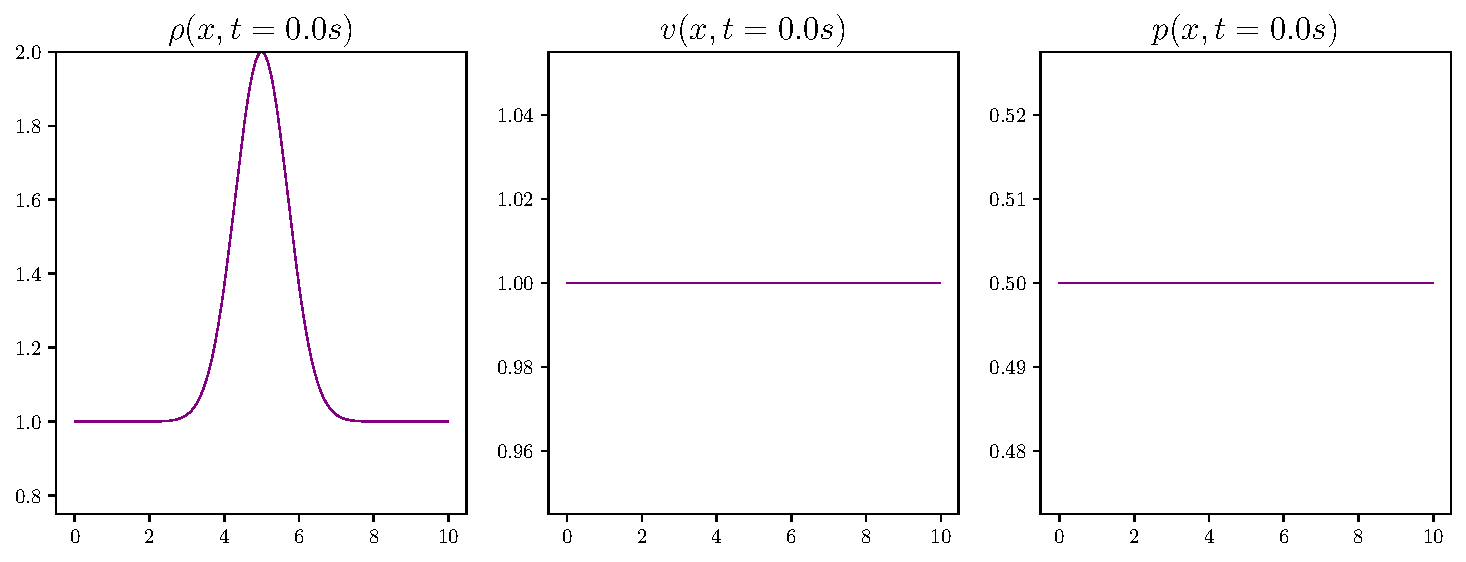
\includegraphics[width=1\linewidth]{../euler1D/plots_en_TDG/set1/graficas/1.pdf}
	\caption{Gráficas para $t=0.0\unit{\s}$}
\end{figure}
\begin{figure}[ht]
	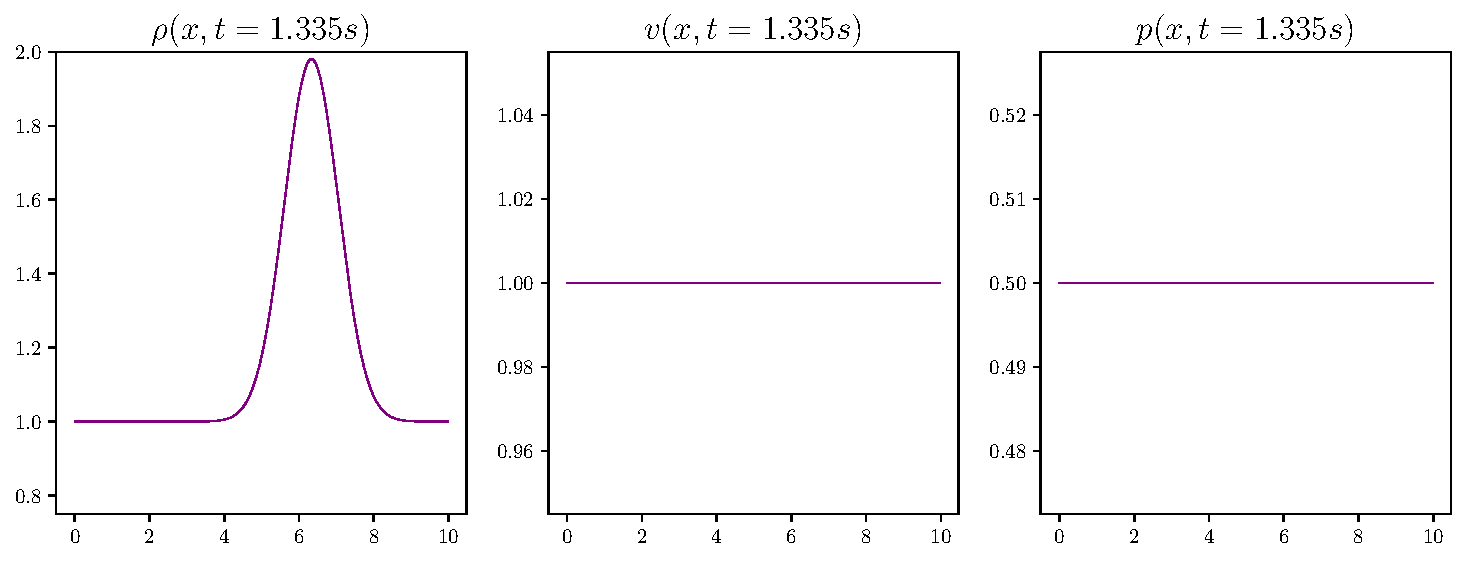
\includegraphics[width=1\linewidth]{../euler1D/plots_en_TDG/set1/graficas/135.pdf}
	\caption{Gráficas para $t=1.335\unit{\s}$}
\end{figure}\vspace{\baselineskip}
\begin{figure}[ht]
	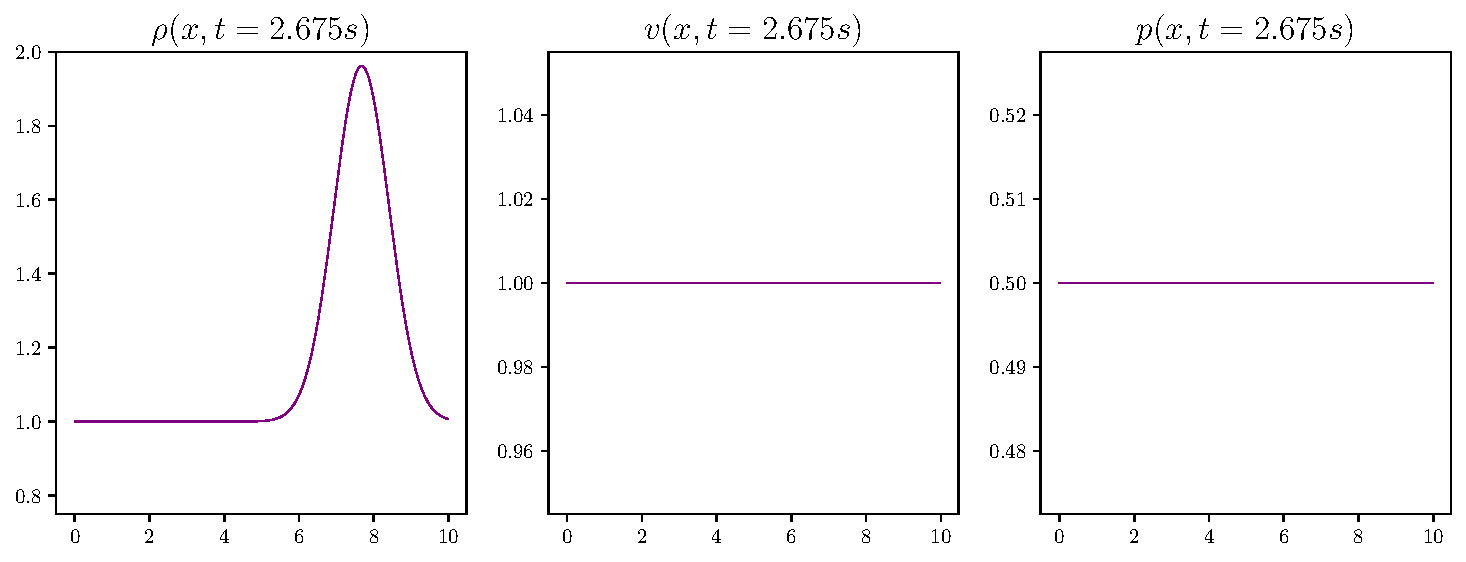
\includegraphics[width=1\linewidth]{../euler1D/plots_en_TDG/set1/graficas/269.pdf}
	\caption{Gráficas para $t=2.675\unit{\s}$}
\end{figure}\vspace{\baselineskip}
\begin{figure}[ht]
	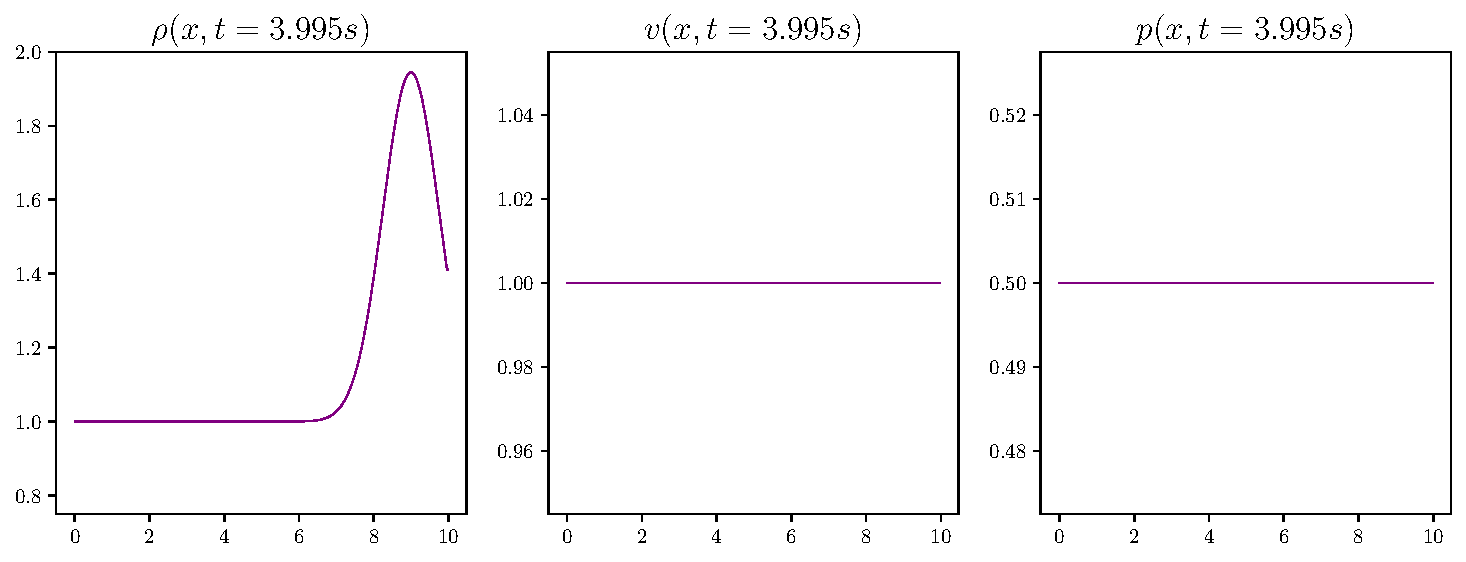
\includegraphics[width=1\linewidth]{../euler1D/plots_en_TDG/set1/graficas/401.pdf}
	\caption{Gráficas para $t=3.995\unit{\s}$}
\end{figure}
\subsubsection{Discusión}
Es apreciable el comportamiento de advección que sufre el perfil gaussiano de la densidad del gas. En el instante $t=0.0\unit{\s}$ el centro de la curva gaussiana se encuentra en $x=5\unit{\meter}$, mientras que en el instante $t=3.995\unit{\s}$ éste se encuentra aproximadamente en $x=9\unit{\meter}$. Esta última observación coincide con lo esperado, dado que la velocidad del gas es $1.0\unit{\meter\per\s}$ y es constante a lo largo de toda la simulación.
Por otro lado, destaca que el máximo de la función de densidad no se mantiene constante, sino que se reduce. Esto se debe al error numérico de integración del esquema utilizado.

Esta simulación se realizó sin la corrección de entropía del esquema de Roe ya que no presentó ninguna diferencia cuando se aplicaba la corrección.
\subsection{Simulación con el segundo conjunto de condiciones iniciales}
Las siguientes gráficas corresponden a la simulación realizada con las condiciones iniciales descritas en la sección (\ref{sec:sod_con_entropy148}). Este conjunto de condiciones se caracteriza por la diferencia entre las magnitudes de las mitades del dominio. La densidad del lado izquierdo triplica la del lado derecho, al igual que sucede con la presión, mientras que la velocidad inicial del fluido es nula. Entonces este sistema puede ser interpretado como la súbita fusión de dos gases con densidad y presión distinta, o en otras palabras, como un \textbf{choque}.
\subsubsection{Gráficas}
\begin{figure}[ht]
	\centering
	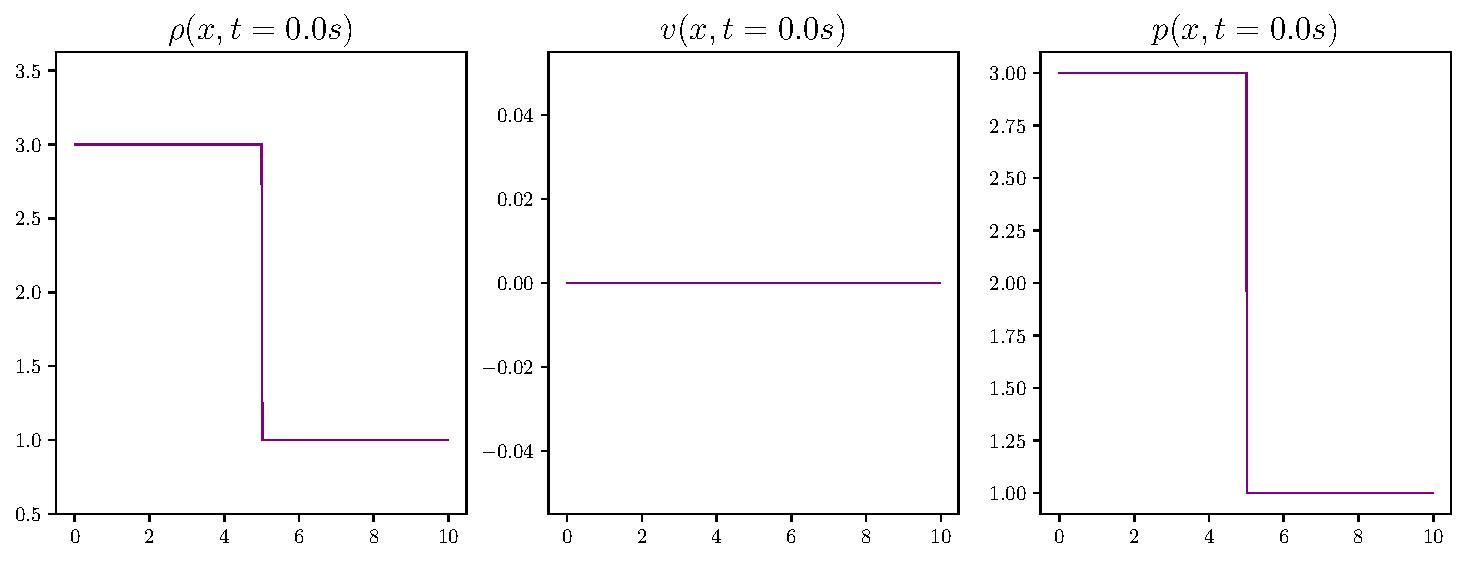
\includegraphics[width=1\linewidth]{../euler1D/plots_en_TDG/set2/1.pdf}
	\caption{Gráficas para $t=0.0\unit{\s}$}
\end{figure}
\begin{figure}[ht]
	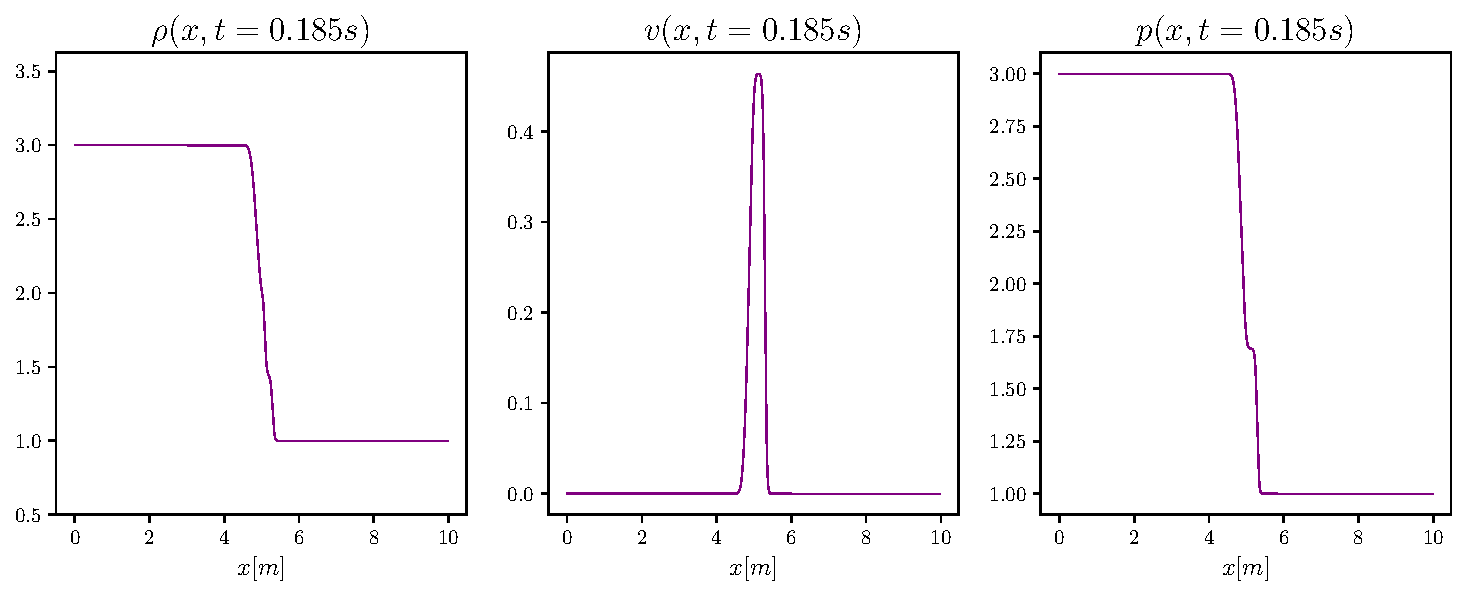
\includegraphics[width=1\linewidth]{../euler1D/plots_en_TDG/set2/20.pdf}
	\caption{Gráficas para $t=0.185\unit{\s}$}
\end{figure}
\begin{figure}[ht]
	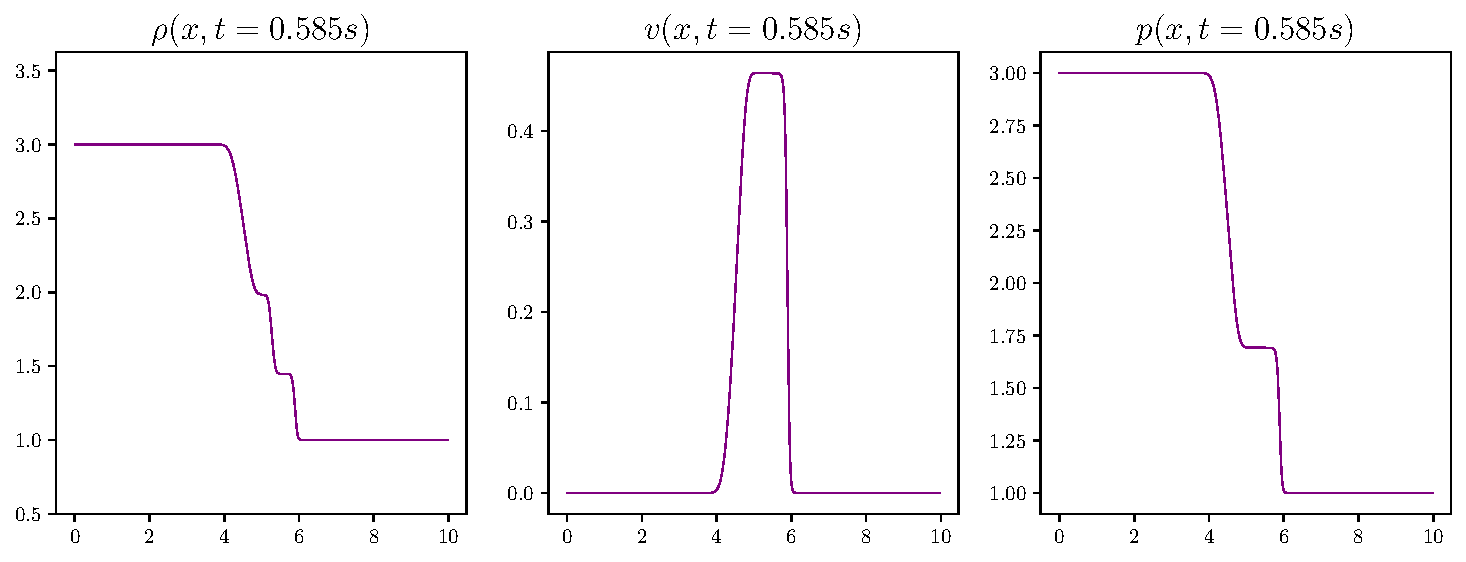
\includegraphics[width=1\linewidth]{../euler1D/plots_en_TDG/set2/60.pdf}
	\caption{Gráficas para $t=0.585\unit{\s}$}
\end{figure}
\begin{figure}[ht]
	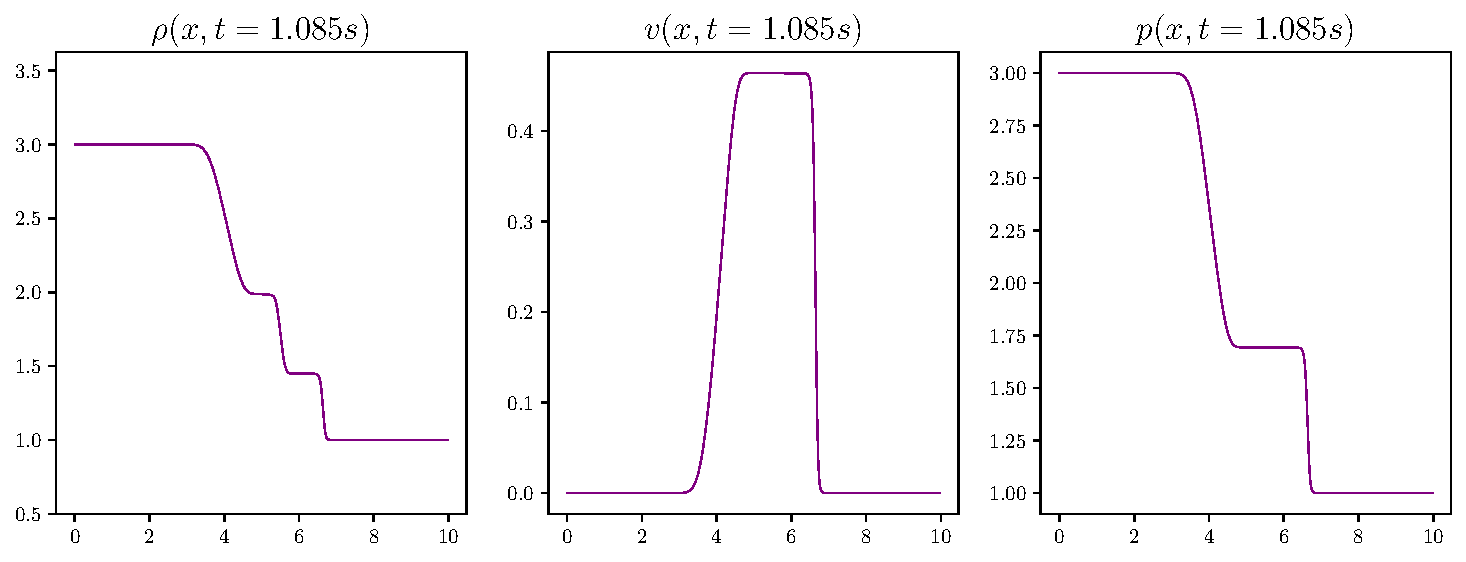
\includegraphics[width=1\linewidth]{../euler1D/plots_en_TDG/set2/110.pdf}
	\caption{Gráficas para $t=1.085\unit{\s}$}
\end{figure}
\subsubsection{Discusión}
En esta simulación se destaca principalmente la manifestación de ondas de choque y de rarefacción en todas las variables del gas. La densidad se divide en tres ondas; una de choque, que avanza hacia la derecha, y otra de rarefacción, que avanza a la izquierda. La onda intermedia entre las dos últimas se conoce como \textbf{discontinuidad de contacto} \cite{thesis-euler-godunov} y se caracteriza por ser una discontinuidad en la densidad únicamente, ya que la presión y velocidad permanecen constantes. La discontinuidad de contacto también está estrechamente relacionada con la diferencia de temperatura entre las partes del gas que ésta divide \cite{LeVeque}. 

Por otro lado, es notable la eficiencia del esquema de Roe al capturar ondas de choque (discontinuidades) como soluciones.

Esta simulación se realizó sin la corrección de entropía del esquema de Roe ya que no presentó ninguna diferencia cuando se aplicaba la corrección.
\subsection{Simulación con el tercer conjunto de condiciones iniciales}
Se experimentó con el conjunto de condiciones iniciales descrito en la sección (\ref{sec:leveque_sin_entropy714}). Este conjunto es similar al discutido anteriormente, con la diferencia que la velocidad inicial de este conjunto no es nula, sino que tiene un valor constante en todo el dominio. Este problema surge a partir de una forma de evaluar la aparición de ondas de rarefacción sónica, de tal manera que pone a prueba la función de corrección de entropía utilizada.

\subsubsection{Gráficas de la simulación sin corrección de entropía}
\begin{figure}[ht]
	\centering
	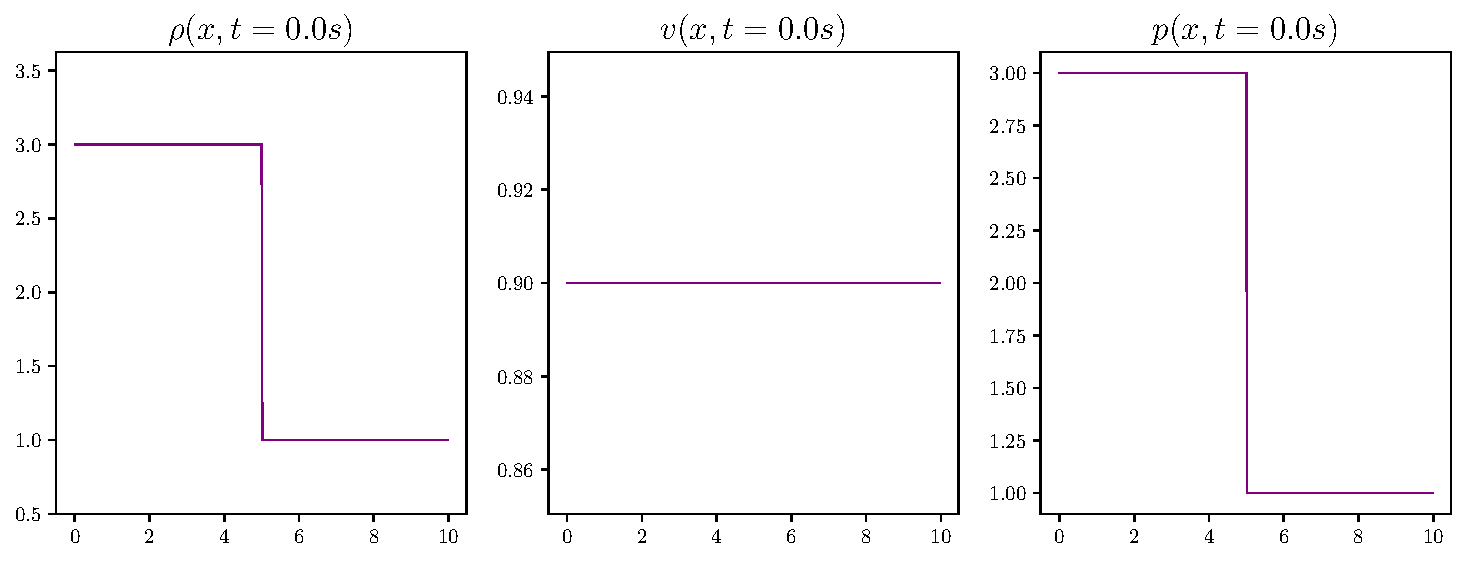
\includegraphics[width=1\linewidth]{../euler1D/plots_en_TDG/set3/leveque_sin_entropy714/1.pdf}
	\caption{Gráficas para $t=0.0\unit{\s}$}
\end{figure}
\begin{figure}[ht]
	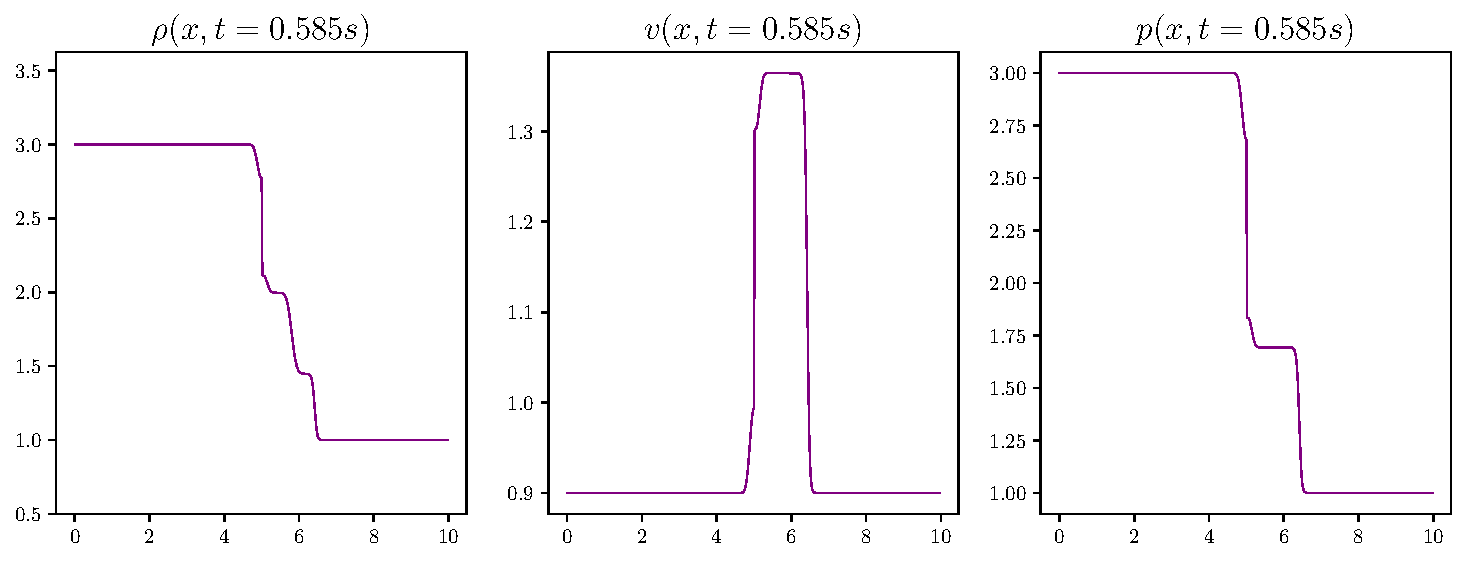
\includegraphics[width=1\linewidth]{../euler1D/plots_en_TDG/set3/leveque_sin_entropy714/60.pdf}
	\caption{Gráficas para $t=0.585\unit{\s}$}
\end{figure}
\begin{figure}[ht]
	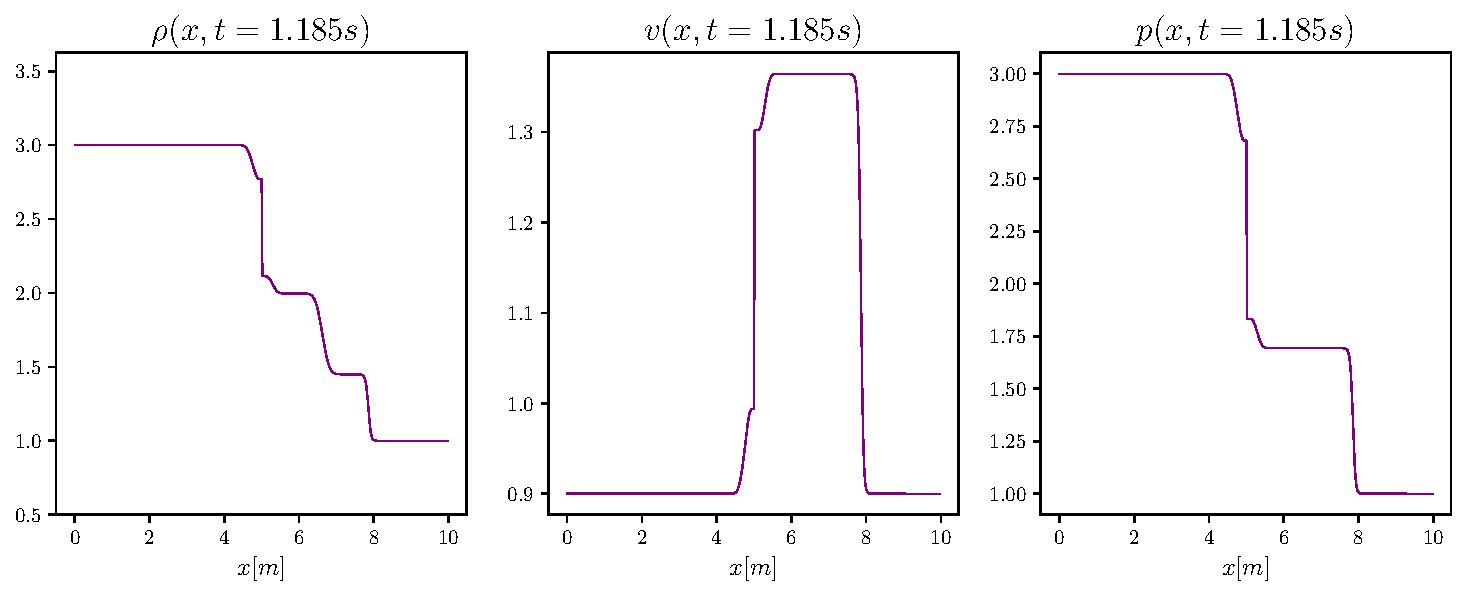
\includegraphics[width=1\linewidth]{../euler1D/plots_en_TDG/set3/leveque_sin_entropy714/120.pdf}
	\caption{Gráficas para $t=1.085\unit{\s}$}
\end{figure}\vspace{\baselineskip}

\subsubsection{Gráficas de la simulación con corrección de entropía}
\begin{figure}[ht]
	\centering
	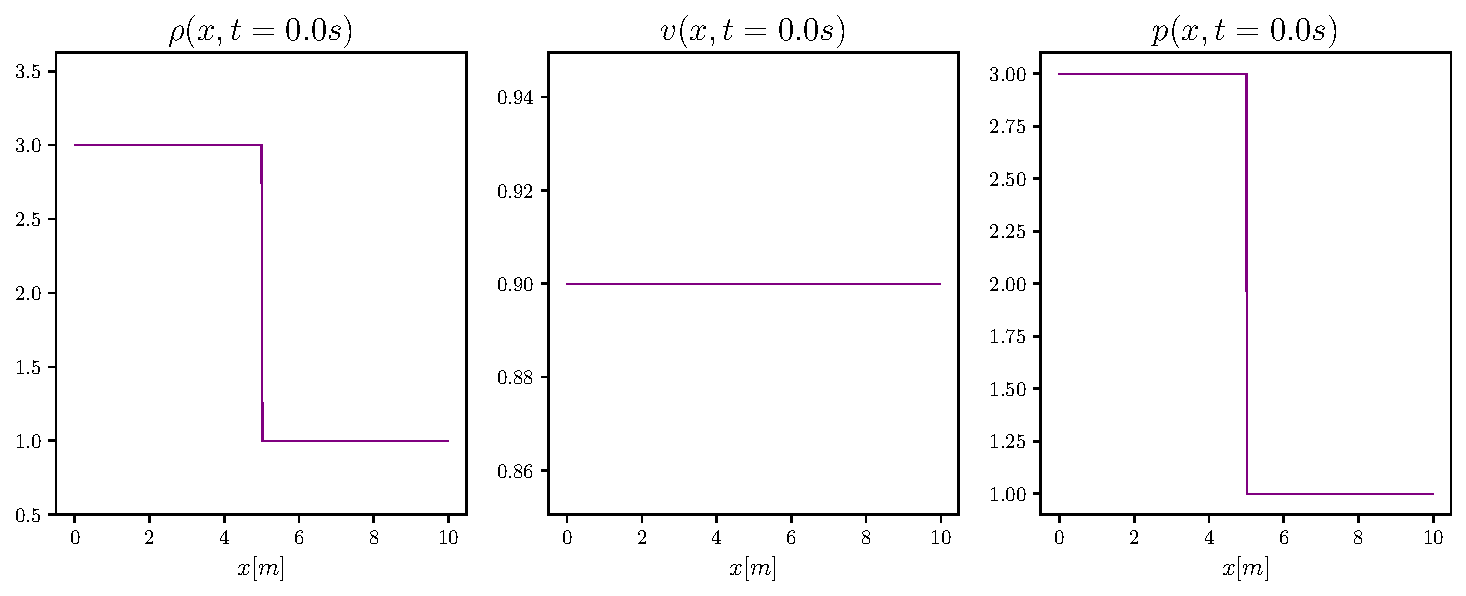
\includegraphics[width=1\linewidth]{../euler1D/plots_en_TDG/set3/leveque_con_entropy123/1.pdf}
	\caption{Gráficas para $t=0.0\unit{\s}$}
\end{figure}
\begin{figure}[ht]
	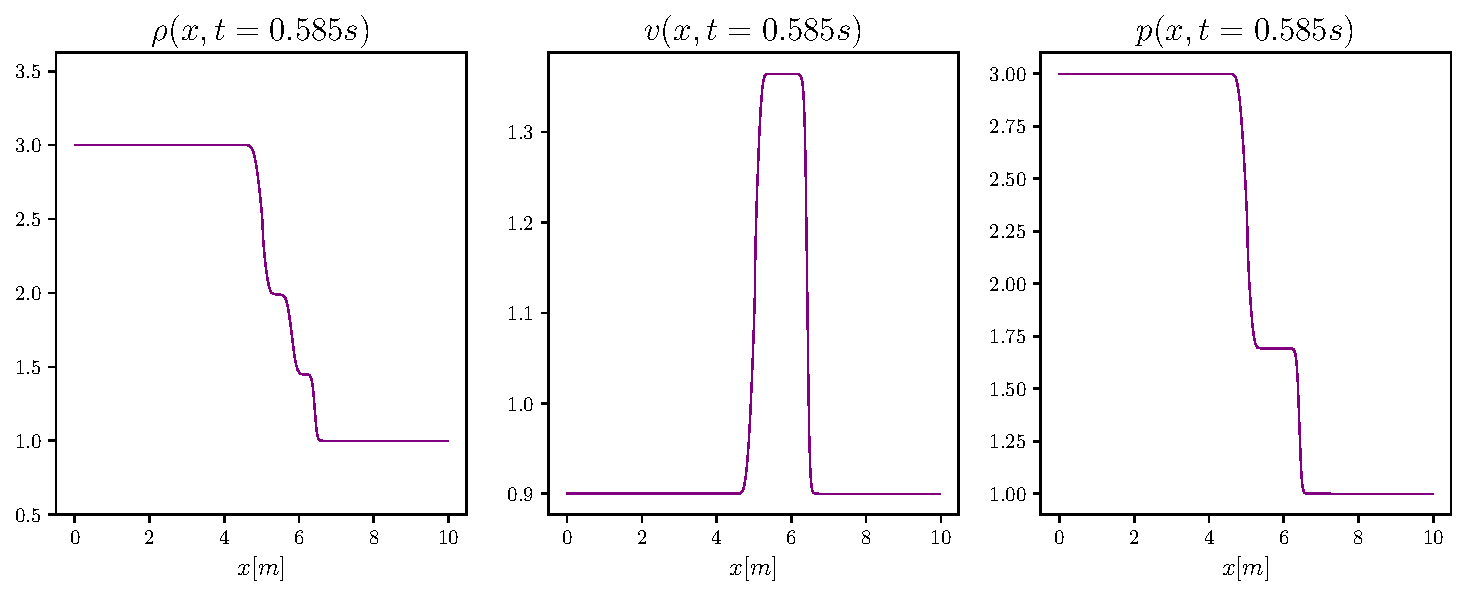
\includegraphics[width=1\linewidth]{../euler1D/plots_en_TDG/set3/leveque_con_entropy123/60.pdf}
	\caption{Gráficas para $t=0.585\unit{\s}$}
\end{figure}
\begin{figure}[ht]
	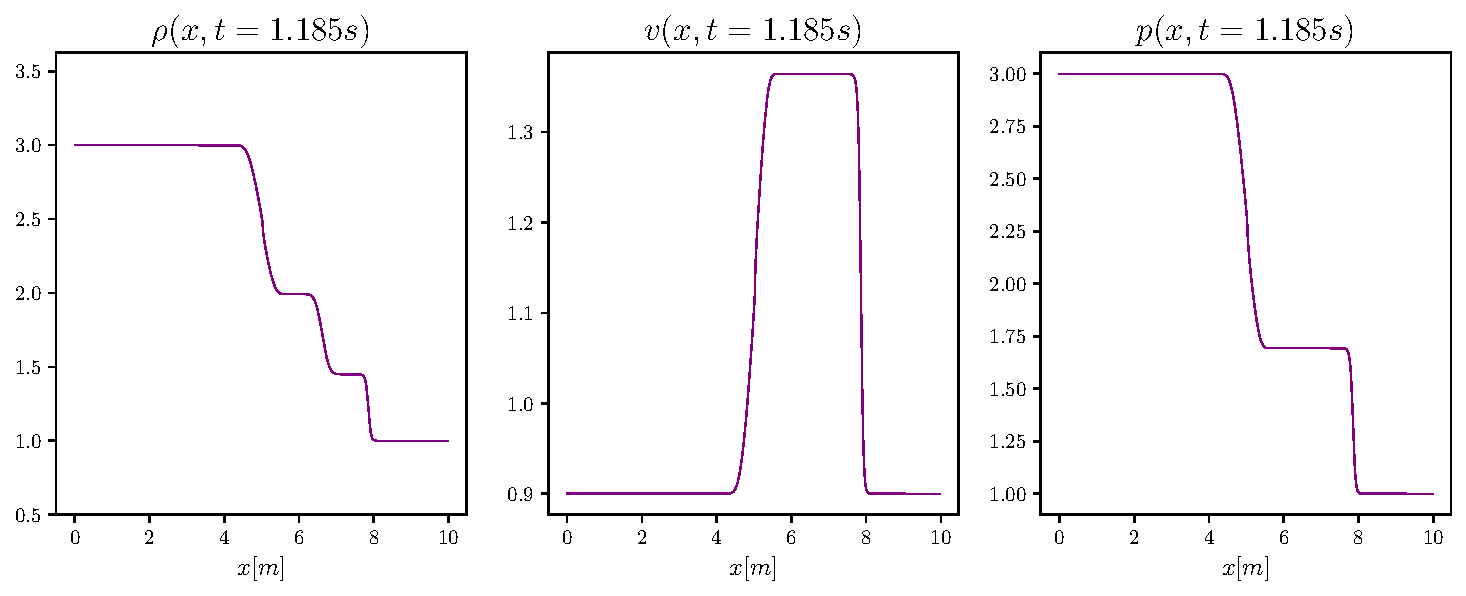
\includegraphics[width=1\linewidth]{../euler1D/plots_en_TDG/set3/leveque_con_entropy123/120.pdf}
	\caption{Gráficas para $t=1.085\unit{\s}$}
	\label{fig:ultima-sin-entropy}
\end{figure}\vspace{5cm}

\subsubsection{Discusión}
Se puede notar la similitud entre los resultados de esta simulación y la correspondiente al segundo conjunto. Sin embargo, en este caso el programa sin la condición de entropía no logra capturar las ondas de rarefacción, como puede notarse en la figura \ref{fig:ultima-sin-entropy}; dado que especialmente la onda de rarefacción que avanza a la izquierda (identificada en los resultados de la sección anterior) aparece dividida por una discontinuidad      % Cap. 3 

\chapter{COMPARACIÓN CON PYCLAW}
Mientras se investigaba sobre las ecuaciones de conservación, previo a la realización de este texto, los textos de Randy LeVeque destacaron por su inmenso aporte a la teoría de la resolución numérica de estos sistemas. Al profundizar en los aportes de LeVeque, fue imposible no toparse con el paquete desarrollado para el lenguaje de programación Python, \textbf{PyClaw}, donde LeVeque está listado como el principal diseñador del software y de los algoritmos implementados \cite{clawpack}. El paquete PyClaw fue desarrollado para la resolución numérica de ecuaciones de conservación lineales y no lineales, utilizando métodos de alta resolución. Estos métodos se basan en la construcción de la solución del problema de Riemann a través de diversos esquemas, como el de Roe.

A continuación se describen los algoritmos implementados en el paquete \textbf{Clawpack}. Esta descripción extrae los conceptos presentados en la documentación oficial del mismo \cite{clawpack}.

\section{Fundamentos de Clawpack}
\textbf{PyClaw} forma parte del paquete de solucionadores numéricos \textbf{Clawpack} \footnote{El nombre abrevia la frase en inglés \textbf{C}onservation \textbf{Law} \textbf{Pack}age.}. Éste es capaz de resolver sistemas de ecuaciones diferenciales de la forma estándar de conservación
\begin{equation}
	q_t + f(q)_x = 0.
\end{equation}

La solución numérica de estos sistemas se basa en solucionadores de Riemann. Sea $S(Q_{i-1}, Q_{i})$ un solucionador de Riemann. Para poder implementar éste último es necesario que retorne un conjunto de $M_{w}$ ondas denominadas $\mathcal{W}_{i-1/2}^{p}$, con velocidades $s_{i-1/2}^{p}$, que correspondan a la solución del problema de Riemann entre las celdas $i$ e $i-1$, siempre que satisfaga la siguiente condición
\begin{equation}
	\sum_{p=1}^{M_{w}}\mathcal{W}_{i-1/2}^{p} = Q_i - Q_{i-1} \equiv \Delta Q_{i-1/2}.
\end{equation}
La construcción, basada en ondas y sus velocidades, de la solución del problema de Riemann se asemeja a la forma en la que se construye la solución para el caso lineal (ver sección \ref{sec:sol-riemann-lineal}). Para calcular la diferencia de flujos que toma lugar en el método de volúmenes finitos, el algoritmo de PyClaw divide la diferencia de flujos en dos fluctuaciones,
\begin{equation}
	\mathcal{A}^{+}\Delta Q_{i-1/2} = \sum_{p}(s_{i-1/2}^{p})^{+}\mathcal{W}_{i-1/2}^{p}
\end{equation}
\begin{equation}
	\mathcal{A}^{-}\Delta Q_{i-1/2} = \sum_{p}(s_{i-1/2}^{p})^{-}\mathcal{W}_{i-1/2}^{p},
\end{equation}
con $s^{-} = \min(s,0)$ y $s^{+} = \max(s,0)$. De tal manera que estas fluctuaciones satisfacen lo siguiente
\begin{equation}
	\mathcal{A}^{+}\Delta Q_{i-1/2} + \mathcal{A}^{-}\Delta Q_{i-1/2} = f(Q_{i})-f(Q_{i-1}).
\end{equation}

Definiendo estos términos, se obtiene una expresión para el esquema general de integración. En la documentación oficial de PyClaw éste se denomina \textbf{Método de Godunov}, pero no debe confundirse con el esquema de Godunov. Entonces,
\begin{equation}
	Q_{i}^{n+1} = Q_{i}^{n} - \frac{k}{h}\left[\mathcal{A}^{+}\Delta Q_{i-1/2} + \mathcal{A}^{-}\Delta Q_{i-1/2}\right]
	\label{eq:pyclaw-scheme}
\end{equation}
es la expresión utilizada en los algoritmos de integración de PyClaw. Cabe resaltar su similitud con \eqref{eq:metodo-vol-finitos-2}, y además implica que la diferencia de flujos numéricos $F(U_{i-1}^n, U_i^n) - F(U_{i}^n, U_{i+1}^n)$ equivale a la suma de las fluctuaciones $\mathcal{A}^{+}\Delta Q_{i-1/2} + \mathcal{A}^{-}\Delta Q_{i-1/2}$ definidas en los algoritmos de PyClaw.

En el software PyClaw se implementa la forma \eqref{eq:pyclaw-scheme} para resolver el sistema de conservación ya que al construir la solución a través de las ondas $\mathcal{W}_{i-1/2}^{p}$ y sus velocidades $s_{i-1/2}^{p}$ es posible implementar métodos de alta resolución. Los métodos de alta resolución introducen valores limitantes para las ondas, de tal manera que se evitan oscilaciones no-naturales cerca de las discontinuidades o también gradientes muy pronunciados o inexactos. Los métodos de alta resolución son métodos numéricos con \textit{variación total disminuida} o métodos \textbf{TVD} por sus siglas en inglés. La forma general de éstos es
\begin{equation}
	Q_{i}^{n+1} = Q_{i}^{n} - \frac{k}{h}\left[\mathcal{A}^{+}\Delta Q_{i-1/2} + \mathcal{A}^{-}\Delta Q_{i-1/2}\right] - \frac{k}{h}\left(\tilde{F}_{i+1/2} - \tilde{F}_{i-1/2}\right),
\end{equation}
donde la corrección de flujos está dada por:
\begin{equation}
	\tilde{F}_{i-1 / 2}=\frac{1}{2} \sum_{p=1}^{M_w}\left|s_{i-1 / 2}^p\right|\left(1-\frac{\Delta t}{\Delta x}\left|s_{i-1 / 2}^p\right|\right) \tilde{\mathcal{W}}_{i-1 / 2}^p .
\end{equation}
Aquí, $\tilde{\mathcal{W}}_{i-1 / 2}^p$ representa la onda ${\mathcal{W}}_{i-1 / 2}^p$ luego de que se le ha aplicado la limitante, de acuerdo al método de alta resolución.
%\clearpage

\section{Código de PyClaw utilizado}
PyClaw ofrece la resolución de las ecuaciones de Euler a través de los algoritmos presentados implementados en Python o incluso mediante Fortran \footnote{Fortran es un lenguaje de programación para cálculos científicos, creado en 1957. Destaca por su eficiencia numérica y sigue siendo útil en aplicaciones científicas.}. Para la resolución de las ecuaciones de Euler se decidió utilizar la versión de Python. En PyClaw están disponibles otros esquemas de flujo numérico distintos al esquema de Roe. Sin embargo, se utilizó de nuevo este esquema para reducir las diferencias entre los programas diseñados (C++ y Python) y basar la comparación en los algoritmos de resolución, principalmente.

\lstinputlisting[
caption = {Paquetes e instancias},
language=Python,
firstline=1,
lastline=9,
keywordstyle=\color{blue}]{../euler1D/code_en_TDG/pyclaw_script.py}
Los paquetes imprescindibles en una simulación de Clawpack son \texttt{pyclaw} y \texttt{riemann}. El solucionador, que implementa la expresión \eqref{eq:pyclaw-scheme}, es un objeto de \texttt{pyclaw} y debe elegirse dependiendo de la dimensión espacial del problema; por ello se utilizó \texttt{ClawSolver1D}. El paquete \texttt{riemann} contiene, como objetos, los sistemas que Clawpack puede solucionar numéricamente. Dichos objetos tienen como métodos los solucionadores de Riemann disponibles.

\lstinputlisting[
caption = {Parámetros básicos de la solución},
language=Python,
firstline=10,
lastline=20,
keywordstyle=\color{blue}]{../euler1D/code_en_TDG/pyclaw_script.py}
Las condiciones de frontera que funcionan como condiciones transmisivas se denominan \texttt{extrap} y se pasan como valores de las listas \texttt{bc\_upper} y \texttt{bc\_lower}, que son atributos del solucionador. El dominio se divide en 500 celdas, al igual que en la simulación de C++, y va de $0\unit{\m}$ a $10\unit{\m}$ horizontalmente. Es posible acceder al punto medio sobre el eje $x$ de cada celda con la lista \texttt{state.grid.p\_centers[0]}.

\lstinputlisting[
caption = {Condiciones iniciales y parámetros auxiliares},
language=Python,
firstline=21,
lastline=37,
keywordstyle=\color{blue}]{../euler1D/code_en_TDG/pyclaw_script.py}
La simulación de PyClaw implementa la resolución de las ecuaciones de Euler en términos de las variables conservadas, i.e., densidad, $\rho$; momentum, $\rho v$ y energía, $\rho E$. Por esta razón, se definieron  las variables físicas independientes y en términos de éstas se asignaron los valores de las variables conservadas. Además, PyClaw exige la definición del coeficiente de dilatación adiabática $\gamma$ como un parámetro del problema como valor del atributo del estado de la solución, \texttt{problem\_data}. Curiosamente, el valor para $\gamma -1$ se asigna por aparte en este mismo atributo.

Por último, el parámetro \texttt{efix} de \texttt{problem\_data} es un booleano que decide si se utilizará la corrección de entropía. Sin embargo, a la fecha no existe ningún algoritmo de corrección de entropía implementado en PyClaw.

\lstinputlisting[
caption = {Ejecución de la simulación},
language=Python,
firstline=38,
lastline=47,
keywordstyle=\color{blue}]{../euler1D/code_en_TDG/pyclaw_script.py}
Para ejecutar la simulación es necesario utilizar un objeto de la clase \texttt{Controller} de \texttt{pyclaw}. En los atributos del objeto se definen otros parámetros relacionados con el tiempo total de simulación y las veces que se imprimen los valores. Cabe destacar que existen atributos del controlador que sirven para indicar el tamaño de paso temporal máximo, ya que hay algoritmos con tamaño de paso temporal adaptativo implementados en la librería.

\section{Comparación de resultados}
Para visualizar la diferencia entre las simulaciones obtenidas con el programa escrito en C++ y las generadas a través de PyClaw se mostrará la superposición de las gráficas de ambas soluciones sobre algunos instantes temporales. 

Por otro lado, para poder cuantificar la diferencia entre las simulaciones se optó por hacer uso del \textbf{error cuadrático medio} entre ambas soluciones. Considerando a $\rho_{i,\texttt{c++}}^{n}$, $u_{i,\texttt{c++}}^{n}$ y $p_{i,\texttt{c++}}^{n}$ como las funciones numéricas producidas por la simulación en C++ y a $\rho_{i,\texttt{py}}^{n}$, $u_{i,\texttt{py}}^{n}$ y $p_{i,\texttt{py}}^{n}$ como las generadas por PyClaw, se define el error cuadrático medio \footnote{RMSE: Root-Mean-Square Error, en inglés.} en el enésimo instante de tiempo, $\text{RMSE}_n$, como:
\begin{equation}
	\text{RMSE}_n(\rho) = \sqrt{\frac{\sum_{i}(\rho_{i,\texttt{c++}}^{n} - \rho_{i,\texttt{py}}^{n})^{2}}{N_x}},
\end{equation}
donde $N_x$ es el número de celdas. La misma fórmula se aplica para las demás variables independientes. Para cuantificar el error total entre simulaciones, se calcula la media cuadrática de los errores cuadráticos previamente definidos. Entonces, se define la cantidad RMSE como
\begin{equation}
	\text{RMSE} = \sqrt{\frac{\sum_{n}^{N_{t}} (\text{RMSE}_{n})^{2}}{N_t}},
\end{equation}
donde $N_t$ es el número de instantes temporales. Este cálculo también se realiza por cada variable. 

Adicionalmente se calculó el error máximo absoluto entre simulaciones, que corresponde a la máxima diferencia absoluta sobre los valores de las funciones numéricas producidas por cada programa. Por ejemplo, el error máximo de la densidad  se calcula como
\begin{equation}
	\text{Error máximo} = \max{(|\rho_{i,\texttt{c++}}^{n} - \rho_{i,\texttt{py}}^{n}|)}.
\end{equation}
\subsection{Comparación del primer conjunto de condiciones iniciales}
\subsubsection{Gráficas}
\begin{figure}[H]
	\centering
	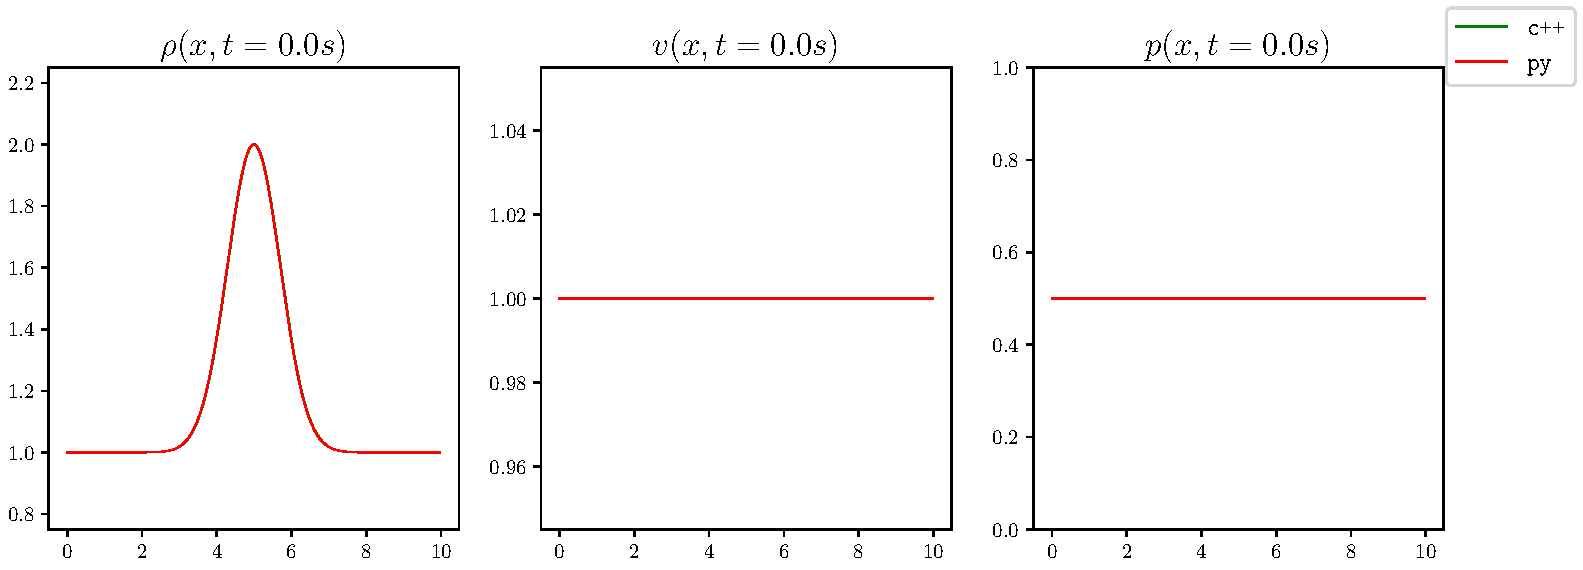
\includegraphics[width=1.1\linewidth]{../euler1D/plots_en_TDG/py_sin_claw/py_gauss199/1.pdf}
	\caption{Gráficas para $t=0.0\unit{\s}$}
\end{figure}

\begin{figure}[H]
	\centering
	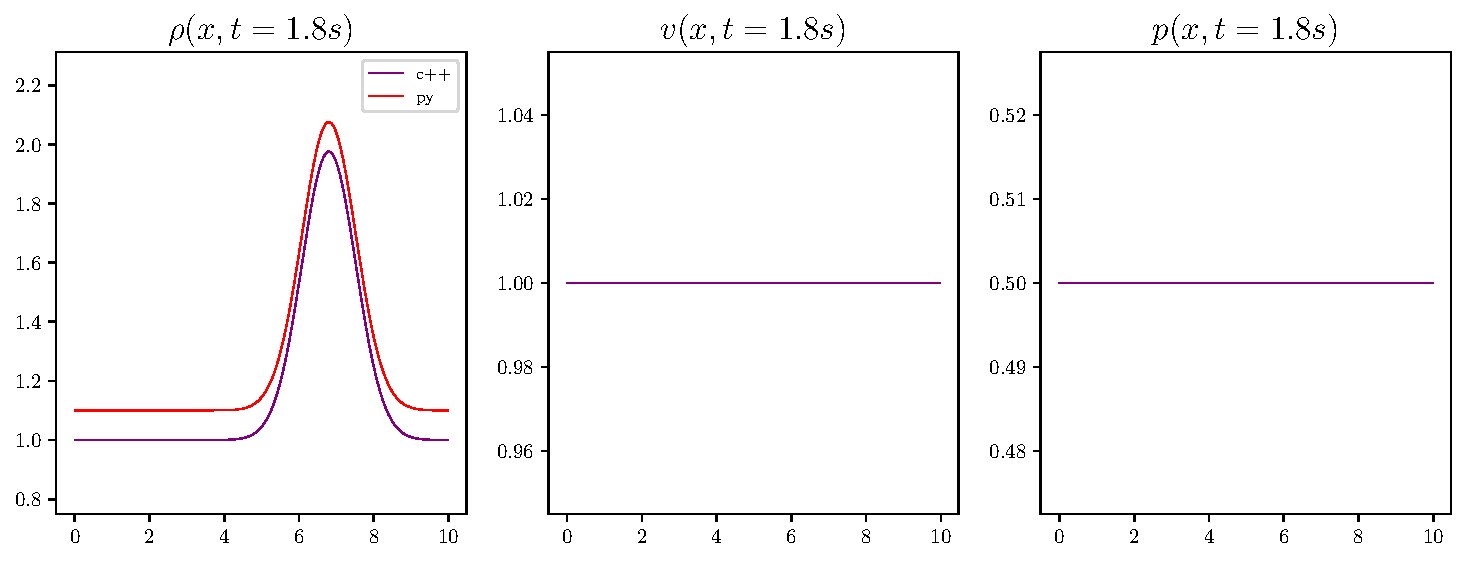
\includegraphics[width=1.1\linewidth]{../euler1D/plots_en_TDG/py_sin_claw/py_gauss199/4.pdf}
	\caption{Gráficas para $t=1.8\unit{\s}$}
\end{figure}

\begin{figure}[H]
\centering
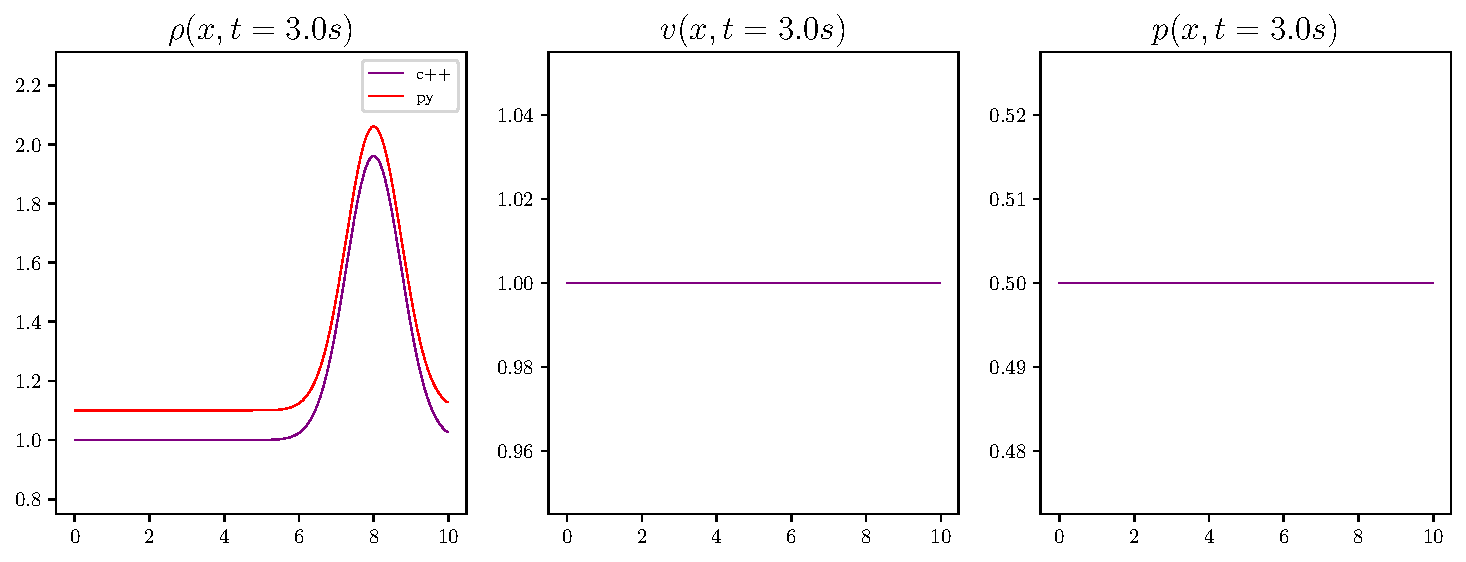
\includegraphics[width=1.1\linewidth]{../euler1D/plots_en_TDG/py_sin_claw/py_gauss199/6.pdf}
\caption{Gráficas para $t=3.0\unit{\s}$}
\label{fig:set-1-py-seg3}
\end{figure}

\begin{table}[ht]
	\large
	\centering
	\begin{tabular}{|l|l|l|l|}
		\hline
		Resultados & $\rho$ & $u$ & $p$ \\ \hline
		RMSE & 8.2e-03 & 0.0e+00 & 0.0e+00 \\ \hline
		Error máximo & 4.1e-02 & 0.0e+00 & 0.0e+00 \\ \hline
	\end{tabular}
	\caption{Comparativa de error entre simulaciones, primer conjunto de condiciones iniciales.}
	\label{tab:tabla-set-1}
\end{table}

\subsubsection{Discusión del primer conjunto de condiciones iniciales}
Se puede notar cómo la simulación de PyClaw sí mantiene la forma original de la campana gaussiana correspondiente a la densidad. En la figura \ref{fig:set-1-py-seg3} es apreciable que el máximo de las dos funciones difiere. Las funciones de velocidad y presión no presentan diferencias entre las dos simulaciones.


\subsection{Comparación del segundo conjunto de condiciones iniciales}
\subsubsection{Gráficas}
\begin{figure}[H]
	\centering
	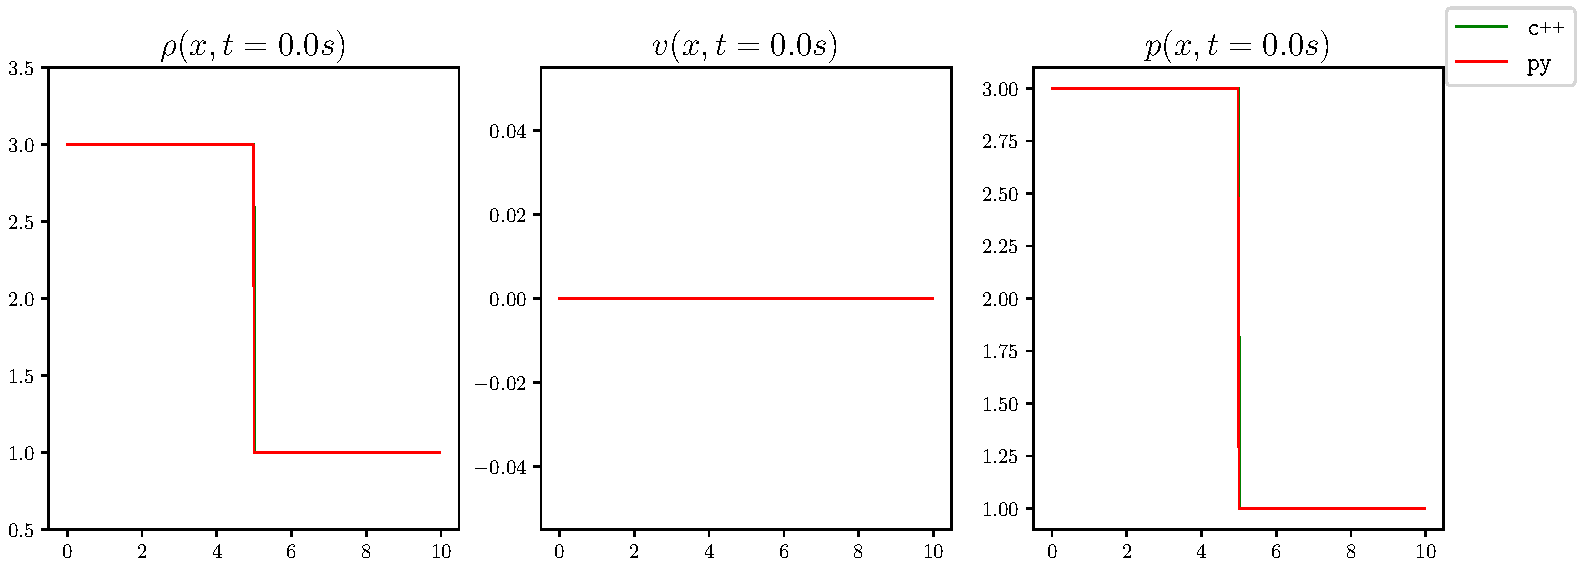
\includegraphics[width=1\linewidth]{../euler1D/plots_en_TDG/py_sin_claw/py_sod659/1.pdf}
	\caption{Gráficas para $t=0.0\unit{\s}$}
\end{figure}
\begin{figure}[H]
	\centering
	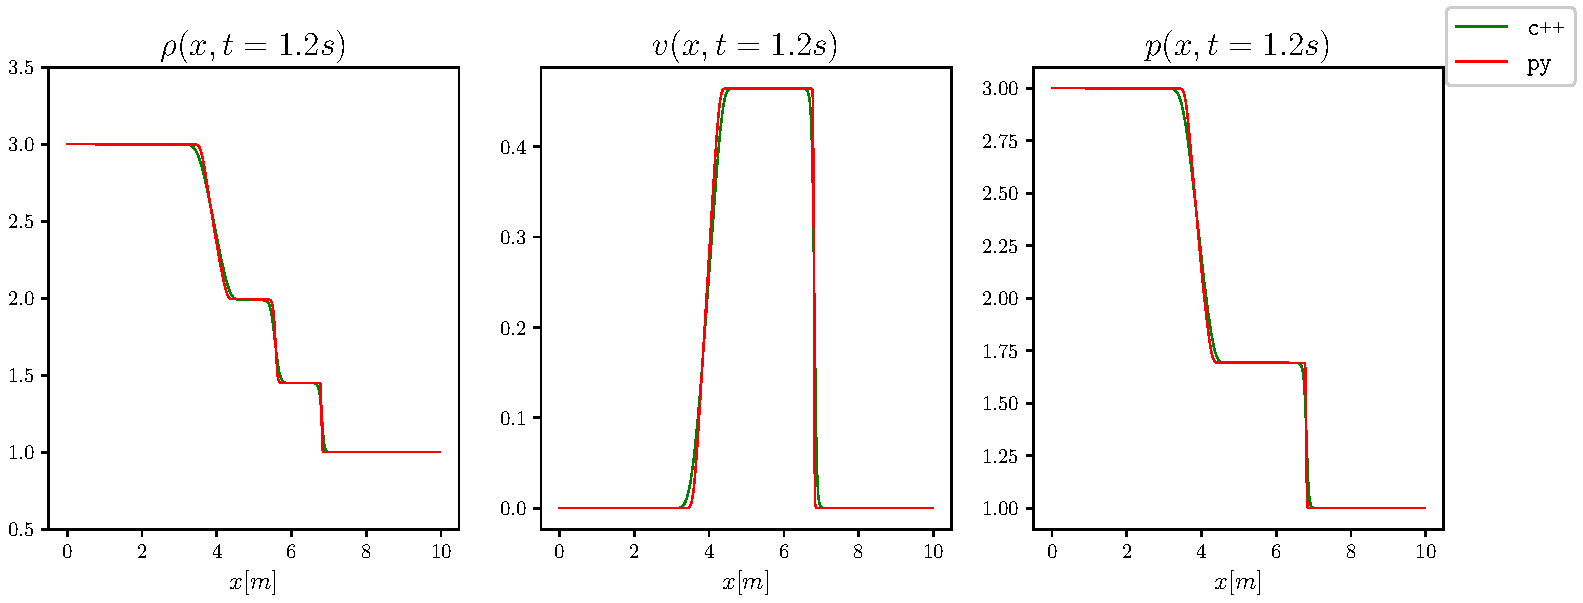
\includegraphics[width=1\linewidth]{../euler1D/plots_en_TDG/py_sin_claw/py_sod659/4.pdf}
	\caption{Gráficas para $t=1.2\unit{\s}$}
\end{figure}
\begin{figure}[H]
	\centering
	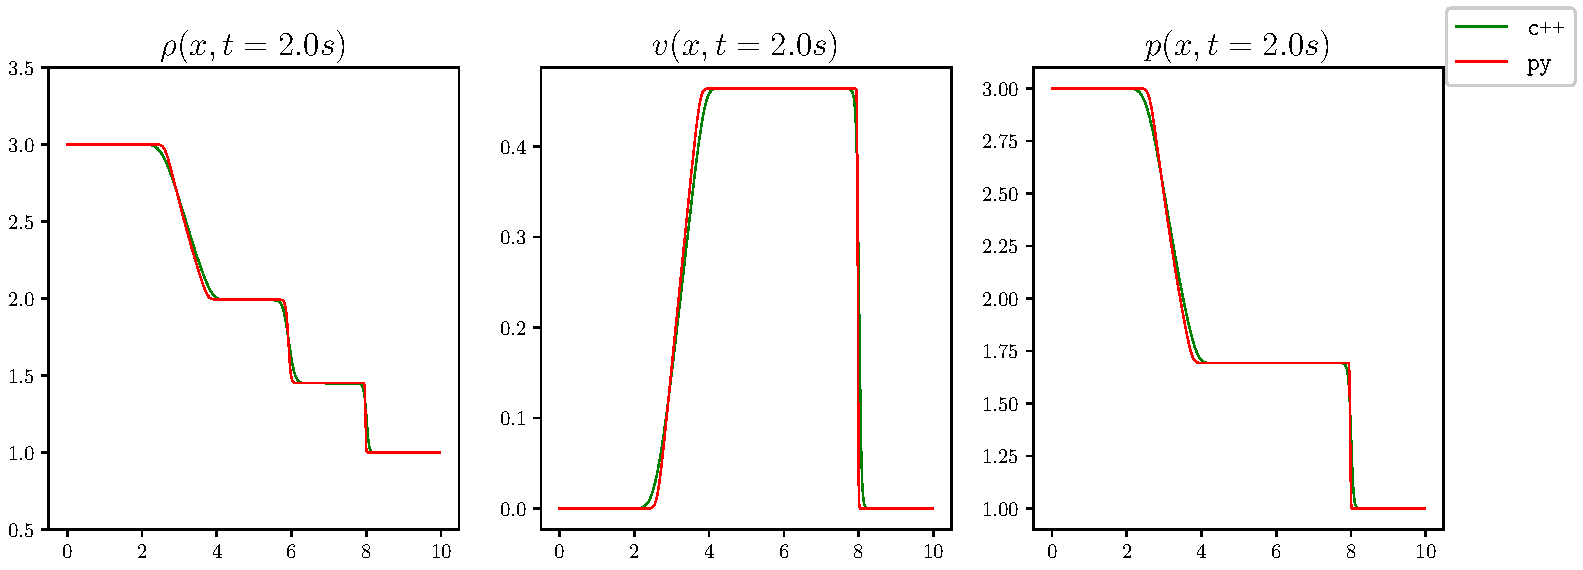
\includegraphics[width=1\linewidth]{../euler1D/plots_en_TDG/py_sin_claw/py_sod659/6.pdf}
	\caption{Gráficas para $t=3.0\unit{\s}$}
\end{figure}\vspace{\baselineskip}
\begin{table}[H]
	\large
	\centering
	\begin{tabular}{|l|l|l|l|} \hline
		Resultados & $\rho$ & $u$ & $p$ \\ \hline
		RMSE & 2.2e-02 & 1.4e-02 & 2.6e-02 \\ \hline
		Error máximo & 1.6e-01 & 1.7e-01 & 2.3e-01 \\ \hline
	\end{tabular}
	\caption{Comparativa de error entre simulaciones, segundo conjunto de condiciones iniciales.}
	\label{tab:tabla-set-2}
\end{table}
\vspace{3\baselineskip}
\subsubsection{Discusión del segundo conjunto de condiciones iniciales}
A través de la simulación con este conjunto de condiciones iniciales se destaca que las funciones producidas por PyClaw devuelven ondas de rarefacción distintas a las producidas por la simulación de C++, notando que poseen pendientes más pronunciadas cerca de las discontinuidades. Este hecho es más evidente al observar la evolución de la presión, ya que es la variable con el valor de RMSE más alto. Se puede inferir que esta diferencia se debe a los algoritmos de alta resolución implementados en PyClaw.

A través de esta simulación resalta que tanto el algoritmo implementado en C++ como los métodos de PyClaw capturan adecuadamente la velocidad de propagación de las ondas de choque y de rarefacción. Este hecho es importante dado que garantiza que los métodos implementados son conservativos.
\clearpage
%
\subsection{Comparación del tercer conjunto de condiciones iniciales}
\subsubsection{Gráficas}
\begin{figure}[H]
	\centering
	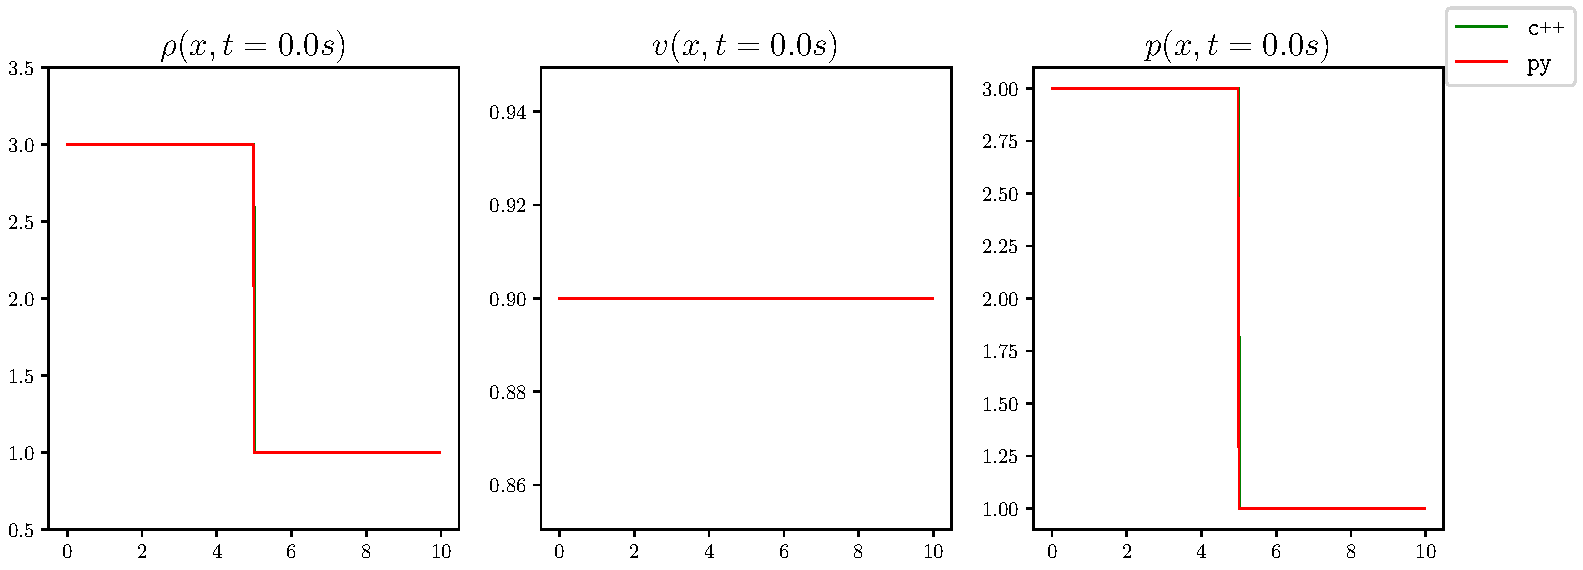
\includegraphics[width=1\linewidth]{../euler1D/plots_en_TDG/py_sin_claw/py_leveque518/1.pdf}
	\caption{Gráficas para $t=0.0\unit{\s}$}
\end{figure}
\begin{figure}[H]
	\centering
	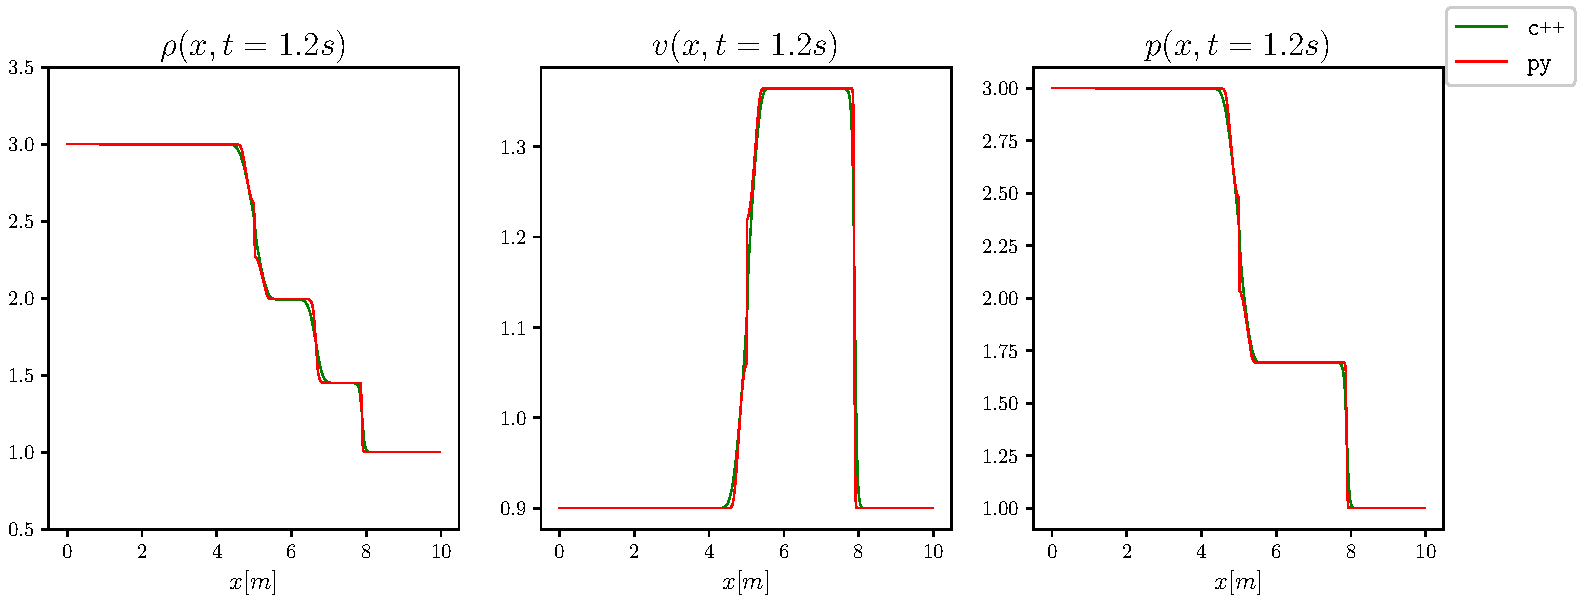
\includegraphics[width=1\linewidth]{../euler1D/plots_en_TDG/py_sin_claw/py_leveque518/4.pdf}
	\caption{Gráficas para $t=1.2\unit{\s}$}
\end{figure}
\begin{figure}[H]
	\centering
	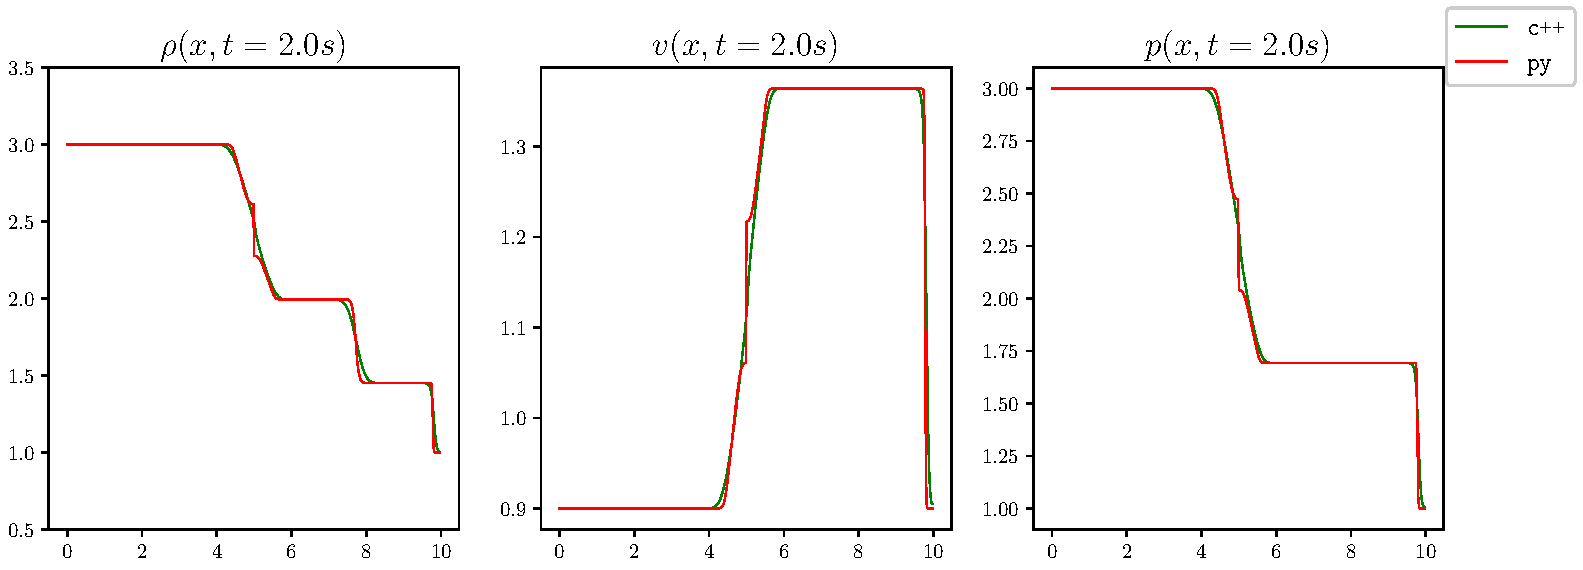
\includegraphics[width=1\linewidth]{../euler1D/plots_en_TDG/py_sin_claw/py_leveque518/6.pdf}
	\caption{Gráficas para $t=2.0\unit{\s}$}
\end{figure}
\begin{table}[H]
	\large
	\centering
	\begin{tabular}{|l|l|l|l|}
		\hline
		Resultados & $\rho$ & $u$ & $p$ \\ \hline
		RMSE & 2.5e-02 & 1.4e-02 & 2.6e-02 \\ \hline
		Error máximo & 2.5e-01 & 1.6e-01 & 3.2e-01 \\ \hline
	\end{tabular}
	\caption{Comparativa de error entre simulaciones, tercer conjunto de condiciones iniciales.}
\end{table}
\subsubsection{Discusión del tercer conjunto de condiciones iniciales}
En este conjunto de soluciones se expone una diferencia que ya había sido observada en los resultados de la simulación con C++ con la corrección de entropía y sin ésta (sección \ref{sec:set-3-cpp}). El algoritmo de PyClaw no considera la corrección de entropía en el esquema de Roe, a diferencia del programa escrito en C++, que sí tiene esta funcionalidad. Por estas razones, este conjunto de soluciones son las que presentan los mayores RMSE. Aunque los errores máximos encontrados no parecen alarmantes, si se dejara correr la simulación por más tiempo, se esperaría que el error aumentara considerablemente. 

\chapter{SIMULACIONES CON DISTINTOS COEFICIENTES DE DILATACIÓN ADIABÁTICA}
\label{cap:5}
En este último capítulo se comparan los resultados obtenidos en simulaciones del mismo problema de condición inicial pero con distinto coeficiente de dilatación adiabática $\gamma$, con el fin de obtener una intuición física, a través de la simulación, de cómo varía el comportamiento de un gas cuando el número de grados de libertad interno del mismo cambia.
\section{Consideraciones preliminares}
Dado que el coeficiente de dilatación adiabática está relacionado explícitamente con el número de grados de libertad interno de un gas $\alpha$,
\begin{equation}
	\gamma = \frac{\alpha + 2}{\alpha},
\end{equation}
es conveniente definir distintos valores para $\gamma$ que dependan de un valor razonable para $\alpha$.

En las anteriores simulaciones, se calculó $\gamma$ para un gas diatómico como el aire. La justificación del número de grados de libertad de estos gases se dio en la sección \ref{sec:ecuacion-de-estado-gas}. En este caso:
\begin{equation}
	\alpha = 5 \implies \gamma = 7/5 = 1.4.
\end{equation}
Entonces, se considerarán experimentos de gases con 16 y 32 grados de libertad internos, que corresponden a $\gamma=1.125$ y $\gamma=1.0625$ respectivamente.
\section{Test de Sod}
El problema de condiciones iniciales que se estudiará con simulaciones con distintos valores para $\gamma$ es el test de Sod (sección \ref{sec:sod_con_entropy148}).
\begin{figure}[H]
	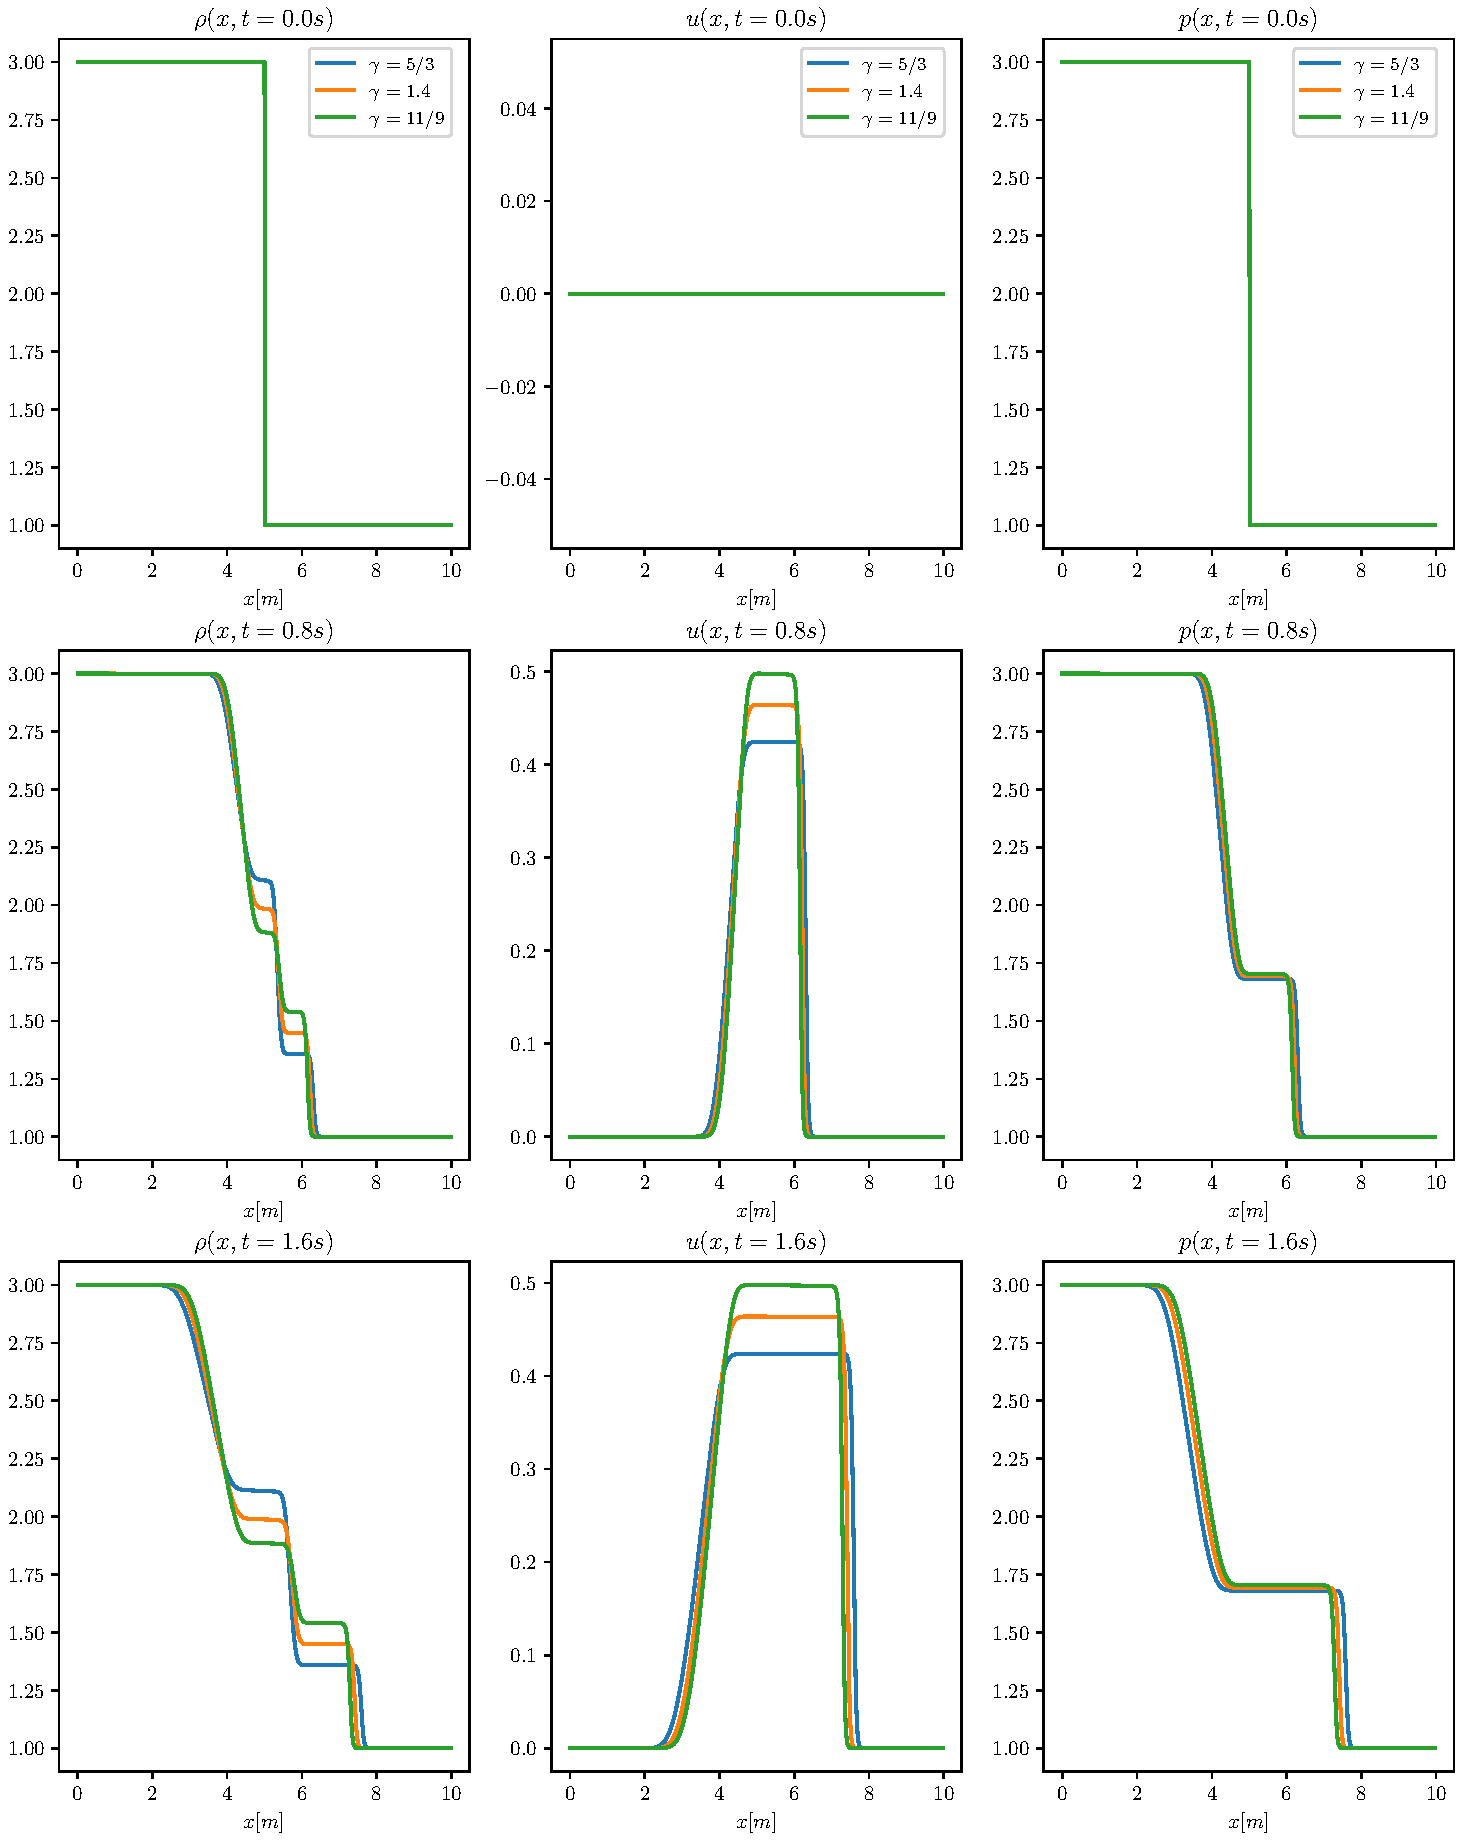
\includegraphics[width=\linewidth]{../euler1D/experimentos/graficas_sod/1.pdf}
	\caption{Primeros tres instantes de las simulaciones con distintos $\gamma$.}
\end{figure}
\begin{figure}[H]
	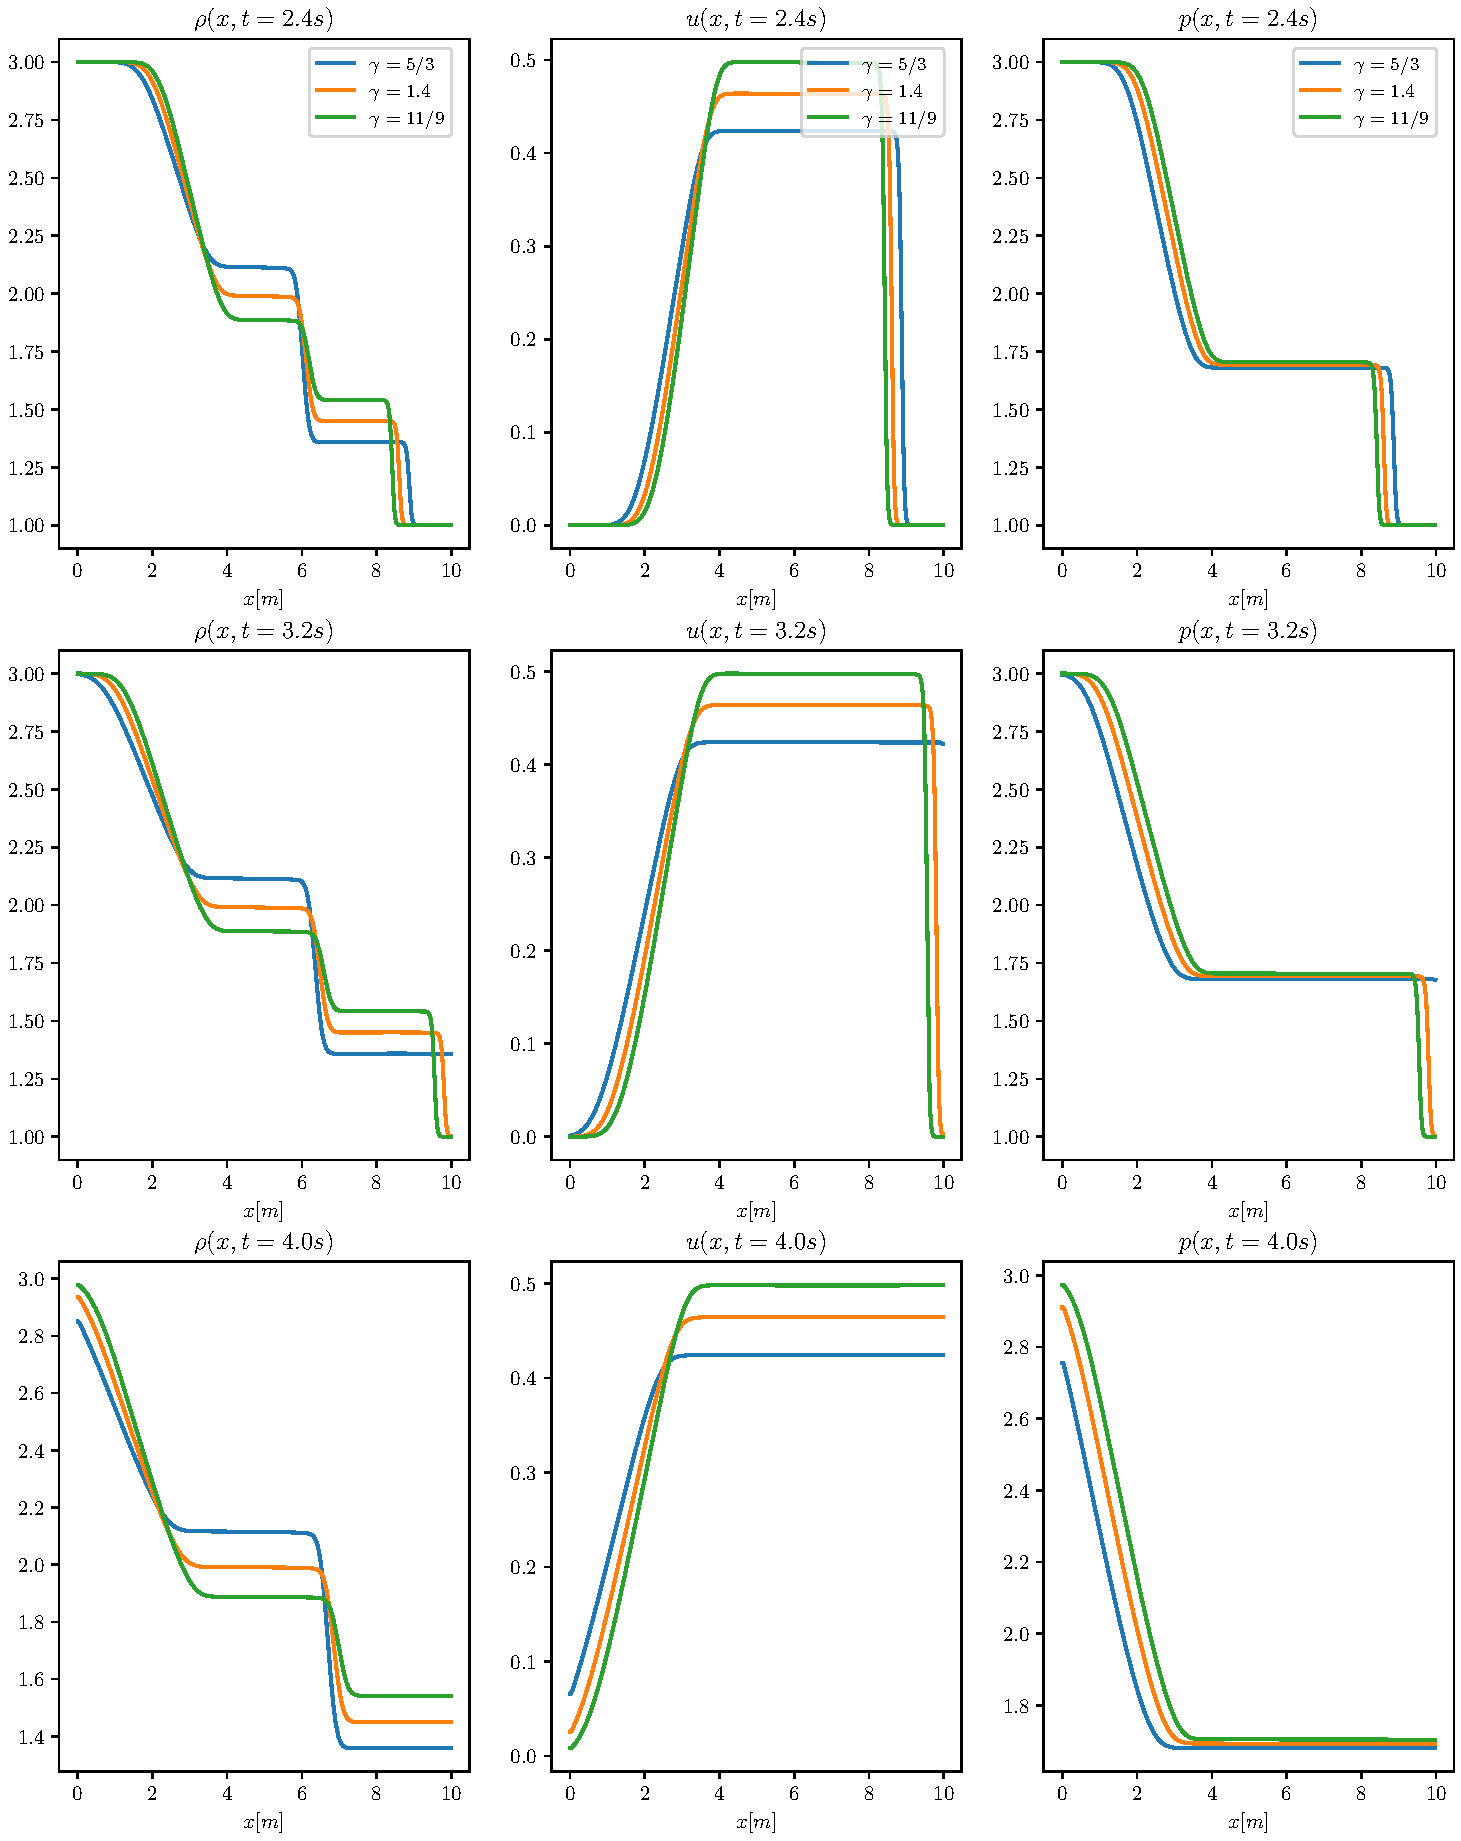
\includegraphics[width=\linewidth]{../euler1D/experimentos/graficas_sod/2.pdf}
	\caption{Últimos tres instantes de las simulaciones con distintos $\gamma$.}
\end{figure}

\subsection{Observaciones}

{\backmatter     %	Capítulos no van numerados --------------------------------------------------  Apartados finales

%%% INCLUYA SUS CONCLUSIONES Y RECOMENDACIONES


\chapter{CONCLUSIONES}
\begin{enumerate}
	\item El método de volúmenes finitos es óptimo para resolver ecuaciones diferenciales de conservación. Sin embargo, debe estudiarse adicionalmente un esquema apto para el cálculo de flujos numéricos aproximados entre las celdas definidas por el método.
	\item El esquema de Roe es un método práctico para resolver numéricamente las ecuaciones de Euler y a través de los promedios de Roe, su implementación es directa. La parte más difícil de completar para implementar el esquema de Roe en la resolución de un sistema de conservación, es encontrar el  promedio adecuado para los autovalores y autovectores de la matriz $\hat{\mathbf{A}}$. Sin embargo, las propiedades que se exigen que cumpla $\hat{\mathbf{A}}$ son sencillas de satisfacer y se pueden usar los promedios de Roe para las ecuaciones de Euler como base.
	\item Las diferencias entre las simulaciones de C++ y PyClaw son menores. Sin embargo, la solución de PyClaw se realiza utilizando técnicas de alta resolución; específicamente, produciendo soluciones a segundo orden de precisión. La principal desventaja al utilizar PyClaw es su ineficiente captura de ondas de rarefacción transónica, dado que la librería no posee algoritmos de corrección de entropía implementados.
	\item El uso de las simulaciones de gases poliatómicos como experimentos, a través de la solución numérica de las ecuaciones de Euler, resulta ser una tarea que brinda intuición física suficiente para entender mejor los fenómenos de los medios continuos. A través de las simulaciones con distintos coeficientes de dilatación adiabática, se pudieron observar efectos que parecían alcanzables únicamente por medio de la solución analítica de los problemas. Además, las variables más abstractas, como la entropía, son más fáciles de comprender mediante una gráfica de la misma, obtenida a través de una simulación.
	\item Las simulaciones numéricas no reemplazan completamente los experimentos de laboratorio. Sin embargo, las simulaciones pueden ser de alta utilidad al hacer comparaciones de gases ficticios, tomando como ejemplo las simulaciones de gases con distintos $\gamma$. Las soluciones numéricas son un recurso de alta utilidad didáctica, especialmente en cursos básicos de la carrera de física, como termodinámica o mecánica.
\end{enumerate}

\chapter{RECOMENDACIONES}
\begin{enumerate}
	\item Se recomienda estudiar a mayor profundidad el método de división de flujos, implementado en PyClaw, con la finalidad de añadir algún algoritmo que realice la corrección de entropía. De preferencia, se propone agregar un conjunto de algoritmos correctores de entropía a disposición del solucionador de Euler. Es posible realizar esta adición, ya que la librería Clawpack es un software de código abierto.
	\item Ya que se estudiaron brevemente algunos esquemas distintos al esquema de Roe, se sugiere adaptar el esquema de Godunov para resolver las ecuaciones de Euler. Esto puede realizarse en un programa de C++ o bien, añadiendo un solucionador exacto en el paquete de Clawpack. Sería apropiado analizar y comparar las soluciones producidas con los esquemas de Roe y Godunov.
	\item Es imprescindible considerar la implementación de métodos de impresión de datos más estandarizados, en el software de Clawpack. Esto se expone como una recomendación porque PyClaw resulta ser ligeramente limitante al momento de imprimir los datos de la solución numérica. Es importante reconocer, de todas maneras, que PyClaw se especializa en producir soluciones gráficas a través del paquete de visualización visClaw.
\end{enumerate}
     % Conclusiones y recomendaciones

\renewcommand{\bibname}{BIBLIOGRAF\'IA}
\nocite{*}			% incluir a todas las entredas bibliográficas
%\bibliographystyle{apacite}	% estilo de bibliografía
\bibliographystyle{flexbib}
\bibliography{bbtesis}   % Bibliografía

}

% Descomentar en el caso de necesitar incluir apéndices
%\appendix			% Apéndices

%\chapter{ECUACIONES DE CONSERVACIÓN Y SISTEMAS HIPERBÓLICOS DE PRIMER ORDEN}
En este capítulo se introducen los conceptos fundamentales de las ecuaciones de conservación y sistemas hiperbólicos de primer orden. Se introduce el problema de Riemann asociado a una ecuación de conservación.
\section{Ecuaciones de conservación}
En física, una ecuación de conservación es una ecuación diferencial parcial de la siguiente forma
\begin{equation}
	\pdv{\mathbf{U}}{t} + \pdv{\mathbf{F}(\mathbf{U})}{x} = 0
	\label{eq:conservacion}
\end{equation}
o utilizando una notación más compacta para las derivadas,
\begin{equation}
	\mathbf{U}_{t} + \mathbf{F}(\mathbf{U})_{x} = 0
	\label{eq:conserv-deriv-short}
\end{equation}
donde $\mathbf{U}$ es un vector n-dimensional de variables físicas que se conservan, por ejemplo, la densidad, la masa o el momentum de un medio \cite{Leveque}. En este texto, las variables de las que depende $\mathbf{U}$ dependen de $x$ y $t$, una variable espacial y otra temporal respectivamente. Por tanto, $\mathbf{U}$ se define formalmente como $\mathbf{U} : \mathbb{R} \times  \mathbb{R} \rightarrow \mathbb{R}^{n}$, mientras que la i-ésima variable conservada se denomina $u_{i}$, de tal manera que $\mathbf{U} = \mathbf{U}(u_{1}, u_{2}, \dots, u_{n})$\hspace{2mm}\cite{Leveque}. 

La función $\mathbf{F}$ corresponde al \textbf{flujo} de cada una de las variables involucradas en un punto $(x,t)$ \cite{Leveque}. Al igual que $\mathbf{U}$, la función $\mathbf{F}$ depende de las mismas variables físicas y por ende, también depende de $(x,t)$. Sin embargo, el flujo de cada variable conservada puede tener una forma distinta, entonces es conveniente escribir a $\mathbf{F}$ como un vector de $n$ funciones independientes, $\mathbf{F} = (f_{1}, f_{2}, \dots, f_{n})$
de tal manera que $f_i$ es la función de flujo de la i-ésima variable conservada, $u_i$ \cite{Leveque}.

Una ecuación de conservación para un sistema definido en un intervalo espacial $D = [a,b]$ necesita de condiciones iniciales para su resolución, el caso más simple a considerar es el de un problema de Cauchy \cite{Leveque}. En dicho caso, se debe especificar una función $\mathbf{U}_0(x)$
\begin{equation}
	\mathbf{U}(x,0) = \mathbf{U}_0(x)
\end{equation} 
la cual sea válida para todo $x$ tal que $x \in D$ y condiciones de frontera
\begin{equation}
	\mathbf{U}(a,t) = \mathbf{U}_{a}
\end{equation}
\begin{equation}
	\mathbf{U}(b,t) = \mathbf{U}_{b}
\end{equation}
con $\mathbf{U}_{a}$ y $\mathbf{U}_{b}$ fijos.

Otra forma de escribir una ecuación de conservación es utilizando la matriz jacobiana $\mathbf{A(\mathbf{U})}$ definida como
\begin{equation}
	\mathbf{A(\mathbf{U})} \equiv
	\begin{bmatrix}
		\pdv{f_1}{u_1} & \dots & \pdv{f_1}{u_n} \\
		\vdots & \ddots & \vdots \\
		\pdv{f_n}{u_1} & \dots & \pdv{f_n}{u_n} \\
	\end{bmatrix}
\end{equation}
de tal manera que la ecuación (\ref{eq:conservacion}) se convierte en
\begin{equation}
	\mathbf{U}_{t} + \mathbf{A(\mathbf{U})}\mathbf{U}_{x} = 0
	\label{eq:conservacion-jacobiana}
\end{equation}.
Esta forma de escribir una ecuación de conservación es relevante ya que permite definir un \textbf{sistema hiperbólico}. Un sistema hiperbólico es una ecuación de conservación de la forma (\ref{eq:conservacion-jacobiana}) tal que los autovalores de la matriz $\mathbf{A(\mathbf{U})}$ para todo $\mathbf{U}$ sean reales y que dicha matriz sea diagonalizable \cite{Leveque}. Esto implica que existen $n$ vectores propios linealmente independientes de $\mathbf{A(\mathbf{U})}$ \cite{Leveque}.
Una ecuación de conservación depende de una función $\mathbf{F(\mathbf{U})}$ que, por lo general, no es una función lineal de $\mathbf{U}$, lo que implica que las ecuaciones de conservación son regularmente no lineales \cite{Leveque}. Esto también se puede inferir por la dependencia en $\mathbf{U}$ de la matriz $\mathbf{A}$ en la ecuación (\ref{eq:conservacion-jacobiana}).
\section{Derivación de una ecuación de conservación}
El principio físico de una ecuación de conservación es más explícito cuando esta se deriva a través de cantidades expresadas en forma \textbf{integral.} Considerando un ejemplo de la mecánica de fluidos, se define $M(x_1,x_2,t)$ como la cantidad de masa de un fluido que se encuentra contenido en un ``tubo'' unidimensional en un intervalo  $[x_1,x_2]$ en un tiempo $t$. Si a dicho fluido se le asocia una densidad $\rho(x,t)$, entonces esta última se define de tal manera que su integral definida en un intervalo espacial sea igual a la masa contenida en ese mismo intervalo \cite{Leveque}, i.e.,
\begin{equation}
	M(x_1, x_2, t) = \int_{x_1}^{x_2}\rho(x,t)\dd{x}.
\end{equation}
Ahora, asumiendo que el tubo es cerrado e impenetrable, la cantidad de masa en una región arbitraria $[x_1,x_2]$ puede variar solamente a causa de que el fluido se desplace (fluya) a través de los puntos límites de la región, $x_1$ y $x_2$ \cite{Leveque}. Para cuantificar el flujo que sale o entra en una región se necesita la velocidad del fluido, $v(x,t)$. Cabe destacar que debido a que el fluido se mueve en un espacio unidimensional, su velocidad se limita a dirigirse en el mismo sentido espacial, es decir, su velocidad tiene dirección sobre $x$. Entonces el flujo del fluido en un punto $(x,t)$, $F(x,t)$, se define como 
\begin{equation}
	F(x,t) = \rho(x,t)v(x,t)
\end{equation}\cite{Leveque}.
Entonces, como previamente se comentó, se puede escribir la razón instantánea de cambio de masa en la región $[x_1,x_2]$ en términos del flujo entrante y saliente de la misma región
\begin{equation}
	\dv{t}	\left[M(x_1, x_2, t)\right] = F(x_2,t) - F(x_1,t)
\end{equation}
\begin{equation}
	\dv{t}	\int_{x_1}^{x_2}\rho(x,t)\dd{x} = \rho(x_2,t)v(x_2,t) - \rho(x_1,t)v(x_1,t)
	\label{eq:continuidad-1-integral}
\end{equation}
Esta es la forma integral de una ecuación de conservación \cite{Leveque}. En particular, esta ecuación refleja el principio de conservación de la masa y a su vez es conocida como \textbf{ecuación de continuidad}. La ecuación (\ref{eq:continuidad-1-integral}) se puede integrar en el tiempo para conseguir expresarla independientemente de cualquier derivada, obteniendo
\begin{equation}
	\int_{t_1}^{t_2}\dv{t}\int_{x_1}^{x_2}\rho(x,t)\dd{x}\dd{t}  = \int_{t_1}^{t_2}\left[\rho(x_2,t)v(x_2,t) - \rho(x_1,t)v(x_1,t)\right]\dd{t}
\end{equation}
\begin{equation}
	\int_{x_1}^{x_2}[\rho(x,t_2) - \rho(x,t_1)]\dd{x}  = \int_{t_1}^{t_2}\left[\rho(x_2,t)v(x_2,t) - \rho(x_1,t)v(x_1,t)\right]\dd{t} 
	\label{eq:continuidad-2-integral}.
\end{equation}
Asumiendo que $t_1<t_2$, esta igualdad ofrece una expresión para la diferencia de masa contenida en la región $[x_1,x_2]$ entre los instantes $t_2$ y $t_1$ \cite{Leveque}. 

Es posible obtener una forma diferencial partiendo de la forma integral de una ecuación de conservación, pero es necesario asumir que las funciones $\rho(x,t)$ y $v(x,t)$ son \textbf{diferenciables}. Esta última característica que se exige en las funciones entra en conflicto cuando se estudian soluciones\footnote{Dichas soluciones se conocen como \textbf{soluciones débiles}, tema que se abordará a detalle más adelante.} de las ecuaciones de conservación con discontinuidades. Por lo tanto, la forma integral de las ecuaciones es utilizada al estudiar problemas con dichas características. Para convertir la ecuación en forma integral a su forma diferencial, se tienen que usar las siguientes expresiones:
\begin{equation}
	\rho(x,t_2)-\rho(x,t_1) = \int_{t_1}^{t_2}\pdv{t}\rho(x,t)\dd{t}
\end{equation}
y
\begin{equation}
	\rho(x_2,t)v(x_2,t)-\rho(x_1,t_1)v(x_1,t) = \int_{x_1}^{x_2}\pdv{x}\rho(x,t)v(x,t)\dd{x}
\end{equation}
sustituyendo estas expresiones en (\ref{eq:continuidad-2-integral}) se obtiene
\begin{equation}
	\int_{t_1}^{t_2}\int_{x_1}^{x_2}\left[\pdv{\rho(x,t)}{t} + \pdv{\rho(x,t)v(x,t)}{x}\right]\dd{x}\dd{t} = 0.
	\label{eq:integral-con-derivadas}
\end{equation}
Puesto que la ecuación (\ref{eq:integral-con-derivadas}) se cumple para cualquier punto $(x,t)$ del dominio, el integrando de la misma debe ser idénticamente cero \cite{Leveque}. Entonces,
\begin{equation}
	\rho_{t} + (\rho v)_{x} = 0
\end{equation}
es la forma diferencial de la ecuación de conservación de la masa, así como se definió una ecuación de conservación en (\ref{eq:conserv-deriv-short}), ya que la función de flujo se definió como $F = \rho v$. Puesto que la ecuación diferencial de conservación de la masa involucra dos cantidades físicas, esta se puede resolver ya sea si se conoce previamente la función $v(x,t)$ o si esta última se puede escribir como una función de $\rho$, i.e., $v=v(\rho)$. En este último caso la ecuación de conservación de la masa es una ecuación diferencial parcial únicamente para $\rho$ \cite{Leveque} y toma la siguiente forma
\begin{equation}
	\rho_t + f(\rho)_x = 0.
\end{equation}
Esta última es un ejemplo de \textbf{ecuación de conservación escalar} \cite{Leveque} ya que solamente interviene una incógnita, $\rho$ \cite{Leveque}.
En caso que la velocidad $v(x,t)$ sea una constante $\alpha$, la ecuación de conservación de la masa se convierte en:
\begin{equation}
	\rho_t + \alpha\rho_x = 0,
	\label{eq:adveccion}
\end{equation}
esta ecuación se conoce como \textbf{ecuación de advección lineal} o como ecuación de onda de primer orden \cite{Leveque}\cite{heattransfer}.
\section{Ecuación de advección lineal}
La ecuación de advección (\ref{eq:adveccion}) con la siguiente condición inicial:
\begin{equation}
	\rho(x,0) = \rho_0(x), \hspace{1.7cm} -\infty < x < \infty,
\end{equation}
tiene como solución:
\begin{equation}
	\rho(x,t) = \rho_0(x - \alpha t),
	\label{eq:sol-advec}
\end{equation}
para $t> 0$, asumiendo que $\rho_0$ es una función diferenciable \cite{Leveque}. Esta solución se puede interpretar como la traslación de la función $\rho_0$ a lo largo del eje $x$ con una velocidad $\alpha$, en la misma dirección de la velocidad, es decir, a la derecha si $\alpha > 0$ y a la izquierda si $\alpha < 0$.
\subsection{Curvas características}
Se puede demostrar que la solución (\ref{eq:sol-advec}) es constante respecto al tiempo a lo largo de cada curva definida por $x-\alpha t = x_0$, para cualquier $x_0$ tal que $x_0 \in [-\infty, \infty]$. Dichas curvas de la forma $x=x(t)$ son conocidas como \textbf{curvas características} de la ecuación diferencial en cuestión \cite{Leveque}. Las curvas características definen dominios en donde la ecuación diferencial parcial se puede escribir como una ecuación diferencial ordinaria. Dichas curvas se definen a partir de ecuaciones diferenciales ordinarias. En el caso de la ecuación de advección lineal (\ref{eq:sol-advec}), las características satisfacen la siguiente ecuación diferencial:
\begin{equation}
	\dv{x}{t} = \alpha, \hspace{1.7cm} x(0) = x_0,
\end{equation}
cuya solución es: $x-\alpha t = x_0$ \cite{Leveque}. Para demostrar que la ecuación de advección lineal se convierte en una ecuación diferencial ordinaria a lo largo de dichas curvas, se deriva la función incógnita $\rho$ respecto al tiempo,
\begin{equation}
	\dv{\rho}{t} = \pdv{\rho}{t} + \pdv{\rho}{x}\dv{x}{t}
\end{equation}
\begin{equation}
	\dv{\rho}{t} = \pdv{\rho}{t} + \alpha\pdv{\rho}{x}
\end{equation}
\begin{equation}
	\dv{\rho}{t} = 0,
\end{equation}
este último paso toma efecto dado que a lo largo de las curvas características, $\dv{x}{t} = \alpha$ \cite{Leveque}. Se puede notar que en este último procedimiento se recuperó la ecuación diferencial en cuestión (\ref{eq:sol-advec}), expresada como una ecuación diferencial ordinaria y concluyó al igualar la derivada temporal a cero, consiguiendo demostrar que $\rho$ es constante a lo largo de las características \cite{Leveque}.
\section{Dominio de dependencia de una ecuación de conservación}
En la sección anterior se introdujo el concepto de curvas características de una ecuación de conservación y en el caso de la ecuación de advección, es posible obtener la solución general utilizando la expresión para sus características, esto es $x(t) = x_0 + \alpha t$. Por lo tanto, se puede afirmar que el valor de $\rho(x,t)$ para un instante $(x',t')$ depende de la condición inicial $\rho_0$ únicamente en un solo punto $x'_{0}$ ya que $\rho$ es constante a lo largo de la curva característica $x' = x^{'}_{0} + \alpha t$ \cite{Leveque}. Entonces, sin importar de qué manera se cambien los valores que toma $\rho_0(x)$, mientras no se cambie su valor en $x'_0$, el valor $\rho(x',t')$ permanecerá sin cambiar \cite{Leveque}. 

En el caso general, para cualquier sistema hiperbólico, el valor de la solución $\mathbf{U}$ en un punto $(x',t')$ depende únicamente de los valores que toma la función inicial $\mathbf{U}_0$ en un dominio $D(x',t')$ que corresponde a un intervalo \textbf{cerrado} \cite{Leveque}. Este último se denomina \textbf{dominio de dependencia} \cite{Leveque}. El tamaño de este intervalo usualmente crece a medida que avance el tiempo, sin embargo, el tamaño está acotado de la siguiente forma $D(x',t') = \{x : |x-x'| \leq a_{\text{máx}}t \}$ \cite{Leveque}. En resumen, las ecuaciones hiperbólicas poseen una velocidad finita de propagación; lo que significa que la información de la solución puede viajar a lo largo del espacio a una velocidad $a_{\text{máx}}$ como máximo \cite{Leveque}.

\section{Discontinuidades en soluciones}
Al derivar la forma diferencial de una ecuación de conservación (\ref{eq:integral-con-derivadas}) se enfatizó que era necesario exigir la diferenciabilidad de las cantidades conservadas. Sin embargo, si se toman en cuenta los atributos de la solución, proporcionados por las curvas características, de la ecuación de advección, resulta que el valor de la variable involucrada $\rho(x,t)$ depende únicamente del valor de la condición inicial en un punto $x_0$ tal que $x = x_0 + \alpha t$ \cite{Leveque}. Por esta última razón se puede concluir que, al menos para la ecuación de advección, es posible definir una solución sin exigirle que sea una función  suave \cite{Leveque}. La definición de una solución con singularidades surge gracias a que la forma integral de una ecuación de conservación sí se satisface con funciones no diferenciables, a diferencia de la forma diferencial \cite{Leveque}. También es importante hacer énfasis en que la forma integral de una ecuación de conservación tiene un significado físico más fundamental.

Si la condición inicial de una ecuación de conservación escalar $u_0(x)$ tiene una singularidad (discontinuidad en sí misma o en alguna derivada), en un punto $x_0$, entonces la solución de la ecuación, $u(x,t)$, también poseerá una singularidad del mismo orden en todos los puntos definidos por la característica que parte de $x_0$ \cite{Leveque}. Para los sistemas hiperbólicos en general, las singularidades se propagan a lo largo de las curvas características \cite{Leveque}.

A continuación se describen dos formas de definir las soluciones con singularidades:
\subsection{Viscosidad disipada}
Como se vio anteriormente algunas soluciones de las ecuaciones de conservación pueden poseer singularidades si la condición inicial de la ecuación tiene una singularidad. Para los sistemas hiperbólicos no lineales, las discontinuidades pueden formarse a lo largo de la evolución temporal de la solución \cite{Leveque}. A las singularidades que se desarrollan en las soluciones se les llama \textbf{ondas de choque} o \textbf{shocks} en inglés \cite{Cameron}. Para definir cómo estas funciones siguen siendo soluciones, en el sentido estricto de la palabra, se redefine la ecuación que deben satisfacer agregándole un coeficiente de viscosidad $\varepsilon$ que va acompañado del laplaciano de la variable involucrada \cite{Leveque}. En el caso de la ecuación de advección para $u$, se define la siguiente ecuación modificada
\begin{equation}
	u_t + \alpha u_x = \varepsilon u_{xx},
	\label{eq:advec-difus}
\end{equation}
donde $u_{xx} \equiv \pdv[2]{u}{x}$ \cite{Leveque}. A esta ecuación se le conoce como \textbf{ecuación de advección - difusión}, ya que el término viscoso también se denomina como término difusivo y está involucrado en la ecuación de difusión, también conocida como ecuación de calor \cite{heattransfer}. 

Si se denota a $u^{\varepsilon}(x,t)$ como la solución de la ecuación (\ref{eq:advec-difus}) con condición inicial $u_0(x)$, entonces $u^{\varepsilon} \in C^{\infty}(\mathbb{R} \times [0,\infty)) $ donde $ C^{\infty}(\mathbb{R}\times [0,\infty))$ es el conjunto de funciones infinitamente diferenciables (suaves) definidas en el mismo espacio en donde se resuelve la ecuación \cite{Leveque}. Esto se cumple incluso si $u_0(x)$ no es una función suave, ya que la ecuación (\ref{eq:advec-difus}) es de tipo parabólica \cite{Leveque}. Para encontrar la solución a la ecuación original (\ref{eq:adveccion}) se debe hacer el límite $\varepsilon \rightarrow 0$ en la solución de la ecuación de advección - difusión (\ref{eq:advec-difus}); a esta forma de definir una solución con discontinuidades se le denomina \textbf{solución con viscosidad disipada} \cite{Leveque}.
\subsection{Solución débil}
La otra forma de definir una solución con singularidades es definiendo una \textbf{solución débil} de la ecuación de conservación, haciendo uso de la forma integral de esta última \cite{Leveque}. Es evidente que la forma diferencial de la ecuación de conservación no se satisface con una función con singularidades ya que sus derivadas no están bien definidas en todo el dominio de la función. La idea del procedimiento de la definición de una solución débil es reescribir la ecuación en forma integral, trasladando las derivadas hacia una \textbf{función prueba}, que sí es una función diferenciable y así relajar las condiciones de suavidad para la función incógnita \cite{Leveque}.

Sea $\phi(x,t)$ una función continuamente diferenciable con \textbf{soporte compacto}, i.e., $\phi(x,t) \in C_{0}^{1} (\mathbb{R} \times [0, \infty))$. La tenencia de soporte compacto de la función significa que $\phi(x,t)$ es exactamente igual a cero fuera de algún conjunto cerrado, por lo que el soporte de la función yace en un subconjunto compacto del espacio $(x,t) = \mathbb{R} \times [0, \infty)$ \cite{Cameron}\cite{Leveque}.

Para definir la solución débil de la ecuación de conservación escalar $u_t + f(u)_x = 0$, esta se multiplica por la función $\phi$ descrita anteriormente:
\begin{equation}
	u_t + f(u)_x = 0
	\label{eq:conser-u}
\end{equation}
\begin{equation}
	\phi u_t + \phi f(u)_x = 0.
\end{equation}
Ahora, se integra sobre todo el espacio y el tiempo,
\begin{equation}
	\int_{0}^{\infty}\int_{-\infty}^{\infty}\left(\phi u_t + \phi f(u)_x\right) \dd{x}\dd{t} = 0,
\end{equation}
luego, integrando por partes cada término de la integral, se obtiene
\begin{equation}
	\int_{-\infty}^{\infty}\int_{0}^{\infty} \phi u_t \dd{t}\dd{x} = \int_{-\infty}^{\infty}\int_{0}^{\infty} \left((\phi u)_t - \phi_t u\right) \dd{t}\dd{x}
\end{equation}
\begin{equation}
	\int_{-\infty}^{\infty}\int_{0}^{\infty} \phi u_t \dd{t}\dd{x} = \int_{-\infty}^{\infty} (\phi u) \Big|_{0}^{\infty}\dd{x} - \int_{-\infty}^{\infty}\int_{0}^{\infty}\phi_t u \dd{t}\dd{x}.
\end{equation}
Dado que $\phi$ tiene soporte compacto, es posible asegurarse que $\lim\limits_{t\rightarrow \infty}\phi(x,t) = 0$. Por tanto,
\begin{equation}
	\int_{-\infty}^{\infty}\int_{0}^{\infty} \phi u_t \dd{t}\dd{x} = 
	-\int_{-\infty}^{\infty} \phi(x,0)u(x,0) \dd{x} - \int_{-\infty}^{\infty}\int_{0}^{\infty}\phi_t u \dd{t}\dd{x}.
\end{equation}
Trabajando el segundo término, se tiene
\begin{equation}
	\int_{0}^{\infty}\int_{-\infty}^{\infty}  \phi f(u)_x \dd{x}\dd{t} = 
	\int_{0}^{\infty}\int_{-\infty}^{\infty} \left((\phi f(u))_x - \phi_x f(u)\right) \dd{x}\dd{t}
\end{equation}
\begin{equation}
	\int_{0}^{\infty}\int_{-\infty}^{\infty}  \phi f(u)_x \dd{x}\dd{t} = 
	\int_{0}^{\infty} \phi f(u) \Big|_{-\infty}^{\infty} \dd{t}  - \int_{0}^{\infty}\int_{-\infty}^{\infty} \phi_x f(u) \dd{x}\dd{t},
\end{equation}
de igual manera que con la valuación de la integral del término anterior, el soporte compacto de $\phi$ permite justificar que $\lim\limits_{x\rightarrow -\infty}\phi = 0 = \lim\limits_{x\rightarrow \infty}\phi$. Entonces,
\begin{equation}
	\int_{0}^{\infty}\int_{-\infty}^{\infty}  \phi f(u)_x \dd{x}\dd{t} =  -\int_{0}^{\infty}\int_{-\infty}^{\infty} \phi_x f(u) \dd{x}\dd{t}.
\end{equation}
Por tanto, la integral de la ecuación de conservación multiplicada por la función prueba queda como
\begin{equation}
\begin{aligned}
	\int_{0}^{\infty}\int_{-\infty}^{\infty}\left(\phi u_t + \phi f(u)_x\right) \dd{x}\dd{t} = \int_{-\infty}^{\infty} \phi(x,0)u(x,0) \dd{x} \\
	-\int_{0}^{\infty}\int_{-\infty}^{\infty}\left(\phi_t u + \phi_x f(u)\right) \dd{x}\dd{t} = 0.
\end{aligned}
\end{equation}
Por tanto, se obtiene la igualdad
\begin{equation}
	\int_{0}^{\infty}\int_{-\infty}^{\infty}\left(\phi_t u + \phi_x f(u)\right) \dd{x}\dd{t} = -\int_{-\infty}^{\infty} \phi(x,0)u(x,0) \dd{x},
	\label{eq:weak-equality}
\end{equation}
que tal y como se dijo previamente, las derivadas parciales ahora están siendo aplicadas a $\phi$ y la integral de la nueva ecuación diferencial se iguala a una integral que depende únicamente de las condiciones iniciales del problema a resolver para $u$. Entonces se dice que $u$ es una \textbf{solución débil} de la ecuación (\ref{eq:conser-u}) si y solo si se cumple la igualdad (\ref{eq:weak-equality}) para todo $\phi$ tal que $\phi(x,t) \in C_{0}^{1} (\mathbb{R} \times [0, \infty))$ \cite{Leveque}.

Es posible demostrar que la igualdad (\ref{eq:weak-equality}) es equivalente a la forma integral de la ecuación diferencial en cuestión (ecuación \ref{eq:continuidad-2-integral}), mediante la elección de una función de prueba que esta cumpla con la siguiente propiedad:
\begin{equation}
	\phi(x,t) = 
	\begin{cases}
		1 & \text{para } (x,t) \in [x_1, x_2] \times [t_1, t_2]\\
		0 & \text{para } (x,t) \notin [x_1 - \epsilon, x_2 + \epsilon] \times [t_1 - \epsilon, t_2 + \epsilon].
 	\end{cases}
\end{equation}
Además $\phi$ es una función suave en la banda intermedia con ancho $\epsilon$ \cite{Leveque}. Entonces al calcular la integral (\ref{eq:weak-equality})  se puede notar que esta se reduce a la integral sobre la banda $\epsilon$, a raíz de la propiedad expuesta anteriormente. Al calcular esta integral y haciendo el límite $\epsilon \rightarrow 0$, las derivadas $\phi_x$ y $\phi_t$ tienden a deltas de Dirac \footnote{La delta de Dirac $\delta(x)$ es una función generalizada que cumple con la siguiente propiedad $\int_{-\infty}^{\infty} \delta(x-a) f(x)\dd{x} = f(a)$ \cite{methods}.}, recuperando así los valores de $u$ y $ f(u)$ en las fronteras del dominio $ [x_1, x_2] \times [t_1, t_2]$ en integrales que equivalen a los términos de la ecuación de conservación en forma integral (\ref{eq:continuidad-2-integral})\cite{Leveque}. Cabe destacar que este es un esbozo solamente de la demostración, ya que esta requiere más rigor matemático. Sin embargo, lo imprescindible es destacar la equivalencia entre ambas expresiones.

La solución de viscosidad disipada también califica como una solución débil y físicamente es la solución correcta \cite{Leveque}. Existen muchas soluciones débiles, incluyendo algunas que no tienen un significado físico consistente, para ello es necesario exigir otras condiciones sobre las soluciones débiles de tal manera que se obtenga la solución correcta \cite{Leveque}. Estas condiciones son conocidas como \texttt{condiciones de entropía} por su papel en la dinámica de fluidos.

\section{Ecuación de Burgers}
Se pueden destacar las propiedades más importantes de las ecuaciones de conservación no lineales de la mecánica de fluidos a través de un ejemplo escalar conocido como \textbf{ecuación de Burgers.} Esta ecuación tiene la siguiente forma:

\begin{equation}
	u_t + u u_x = 0,
	\label{eq:burgers}
\end{equation}
la cual es formalmente conocida como Ecuación de Burgers sin viscosidad \cite{Leveque}, pero en este texto se le referirá solamente como Ecuación de Burgers. Esta ecuación es un modelo muy simple de la velocidad $u$ de un gas \cite{Cameron}. La ecuación originalmente estudiada por Jan Burgers \cite{Leveque} contiene un término de viscosidad cinemática:
\begin{equation}
	u_t + u u_x = \varepsilon u_{xx},
	\label{eq:burgers-vis}
\end{equation}
donde $\varepsilon$ es el coeficiente de viscosidad cinemática. A esta última ecuación se le referirá como Ecuación de Burgers viscosa.

De la ecuación (\ref{eq:burgers}) podemos notar un ligero parecido a la ecuación de advección (\ref{eq:adveccion}), con la diferencia que la velocidad de advección $\alpha$ se reemplaza por la variable que sufre la advección, i.e., $u$ \cite{Leveque}, lo que brinda la naturaleza no lineal de este modelo. La ecuación de Burgers se puede escribir en forma conservativa:
\begin{equation}
	u_t + \left(\frac{1}{2}u^{2}\right)_x = 0.
	\label{eq:burgers-cons}
\end{equation}
A partir de esta forma, se puede concluir que la función de flujo es $f(u) = \frac{1}{2}u^{2}$.
\subsection{Curvas características}
Las curvas características de la ecuación de Burgers se pueden definir a través de la siguiente ecuación diferencial \cite{Leveque}
\begin{equation}
	x'(t) = u(x(t),t),
	\label{eq:burgers-char}
\end{equation}
dado que se puede recuperar la ecuación diferencial parcial derivando respecto al tiempo la velocidad:
\begin{equation}
	\dv{t} u(x(t),t) = \pdv{u}{t} + \pdv{u}{x} \dv{x}{t}
\end{equation}
\begin{equation}
	\dv{t} u(x(t),t) = \pdv{u}{t} + u\pdv{u}{x} = 0.
\end{equation}
Por lo tanto, $u$ es constante en el tiempo sobre cualquier característica. Se puede resolver la ecuación (\ref{eq:burgers-char}) utilizando este último hecho:
\begin{equation}
	x(t) = u(\xi,0)t + \xi
	\label{eq:burg-char-expr}
\end{equation}
y al resolver para $\xi$, es posible resolver la ecuación diferencial \cite{Leveque}
\begin{equation}
	u(x,t) = u(\xi, 0).
	\label{eq:sol-burgers-char}
\end{equation}
Es importante destacar que la expresión (\ref{eq:sol-burgers-char}) para $u(x,t)$ no es válida para todo $t$, dado que las características definidas por la ecuación (\ref{eq:burg-char-expr}) pueden intersectarse en algún momento. Esto se da si para algún $x$, se tiene que $u_0'(x) < 0$ \cite{Leveque}. 

\begin{figure}
	\begin{subfigure}{0.5\textwidth}
		\centering
		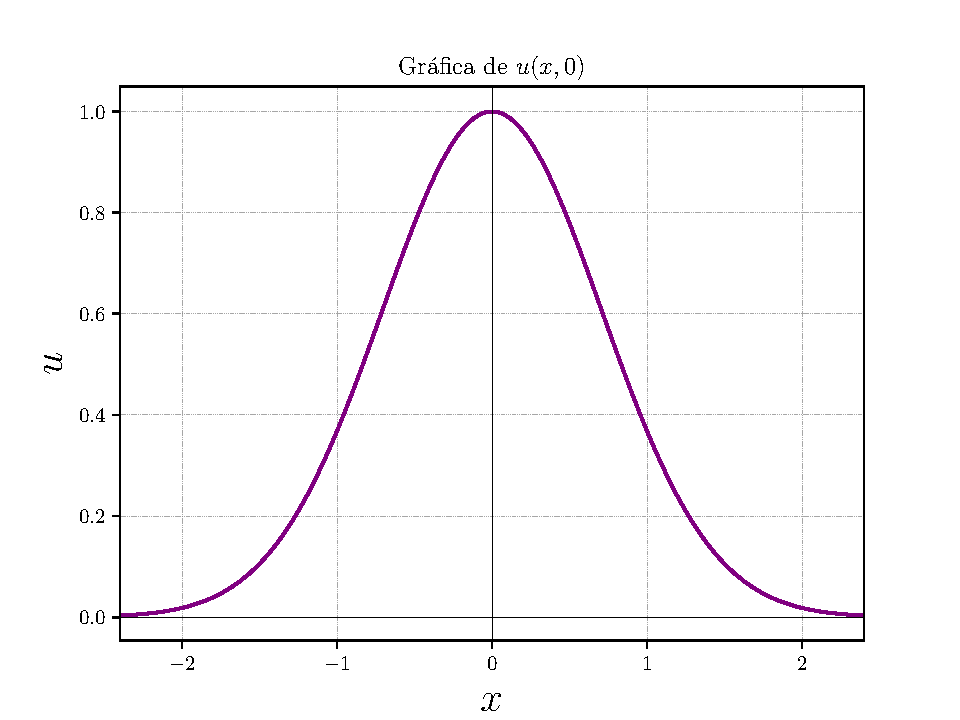
\includegraphics[width=\linewidth]{../some_plots/cond_inicial.pdf}
		\caption{Gráfica de $u(x,0) = \exp(-x^2)$.}
		\label{fig:subfig1}
	\end{subfigure}%
	\begin{subfigure}{0.5\textwidth}
		\centering
		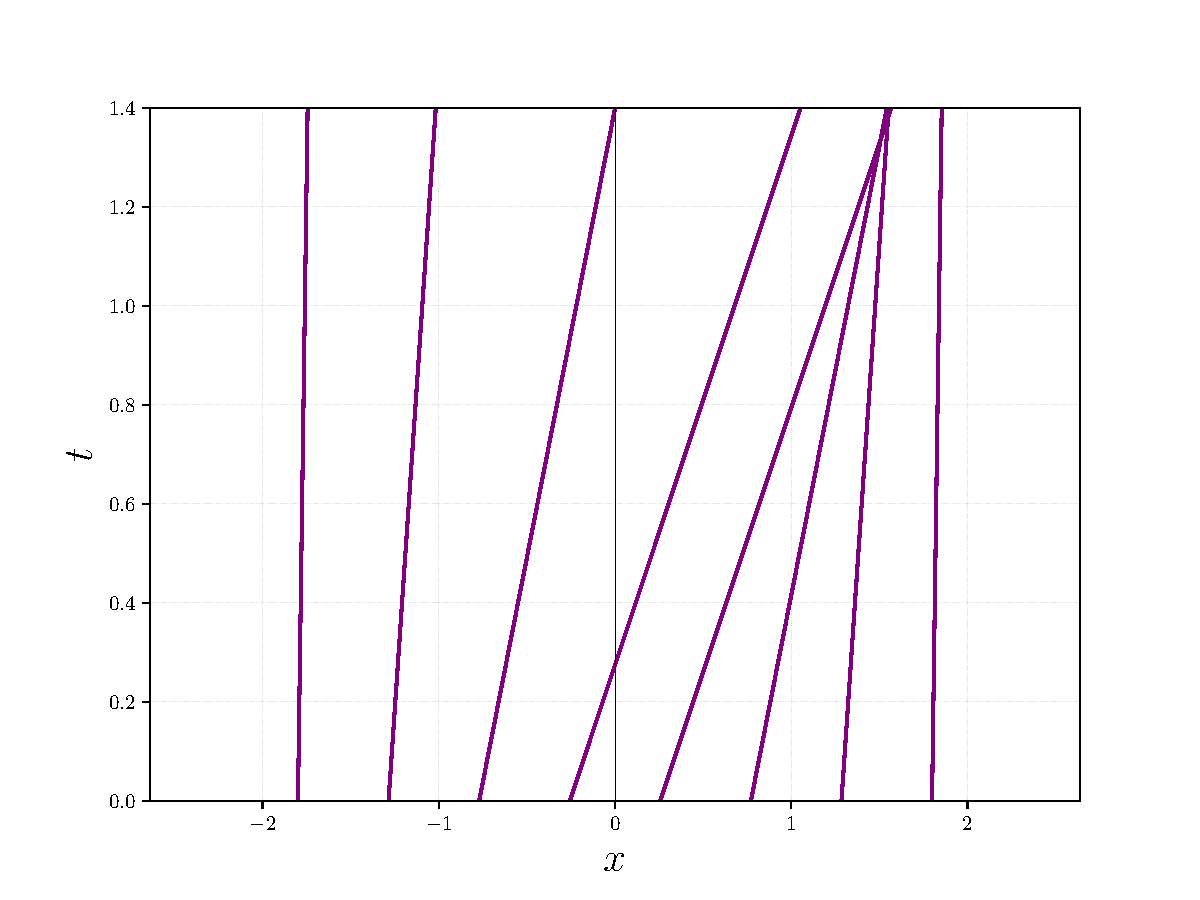
\includegraphics[width=\linewidth]{../some_plots/caracteristicas_burgers.pdf}
		\caption{Características de la ecuación de Burgers.}
		\label{fig:subfig2}
	\end{subfigure}
	\caption{Gráficas de la condición inicial $u(x,0) = \exp(-x^2)$ para la ecuación de Burgers y de algunas características asociadas a esta condición inicial. \textbf{Fuente:} elaboración propia.}
	\label{fig:figura_completa}
\end{figure}
\subsection{Ondas de choque}
Como se puede observar en la figura (\ref{fig:subfig2}), las características asociadas a una condición inicial con forma gaussiana se intersectan. Entonces, si las características se intersectan, la expresión (\ref{eq:sol-burgers-char}) no está bien definida, sino que $u(x,t)$ puede tomar varios valores a la vez, cada uno correspondiente a una característica diferente. En el caso de la ecuación de Burgers, cuando las características se intersectan, la solución se convierte en una ``función'' con tres valores distintos \cite{Leveque}. Esta solución puede tener sentido en algunos contextos, como en el caso del problema de agua superficial \cite{Leveque}. Sin embargo, en la mayoría de casos esta solución no tiene significado físico ya que la variable $u(x,t)$ representa una velocidad y esta debe devolver un solo valor \cite{Leveque}.

La solución con el comportamiento físico correcto cuando las características se intersectan corresponde a una discontinuidad que se propaga con una velocidad determinada \cite{Leveque}. Este efecto se puede demostrar a través del formalismo de la viscosidad disipada. Al obtener la solución de la ecuación de Burgers viscosa (\ref{eq:burgers-vis}), el parámetro $\varepsilon u_{xx}$ evita que la solución presente una discontinuidad, dado que cuando la onda comienza a presentar el choque, la segunda derivada de $u$ crece más rápido que su primera derivada \cite{Leveque}. Así, al efectuar el límite de $\varepsilon \rightarrow 0$ se puede obtener una discontinuidad absoluta que corresponde a la solución de la ecuación de Burgers sin viscosidad. La tendencia de adquirir una discontinuidad  de las soluciones con menos viscosidad se puede evidenciar en la figura (\ref{fig:viscosas}).

\begin{figure}[ht]
	\begin{subfigure}{0.5\textwidth}
		\centering
		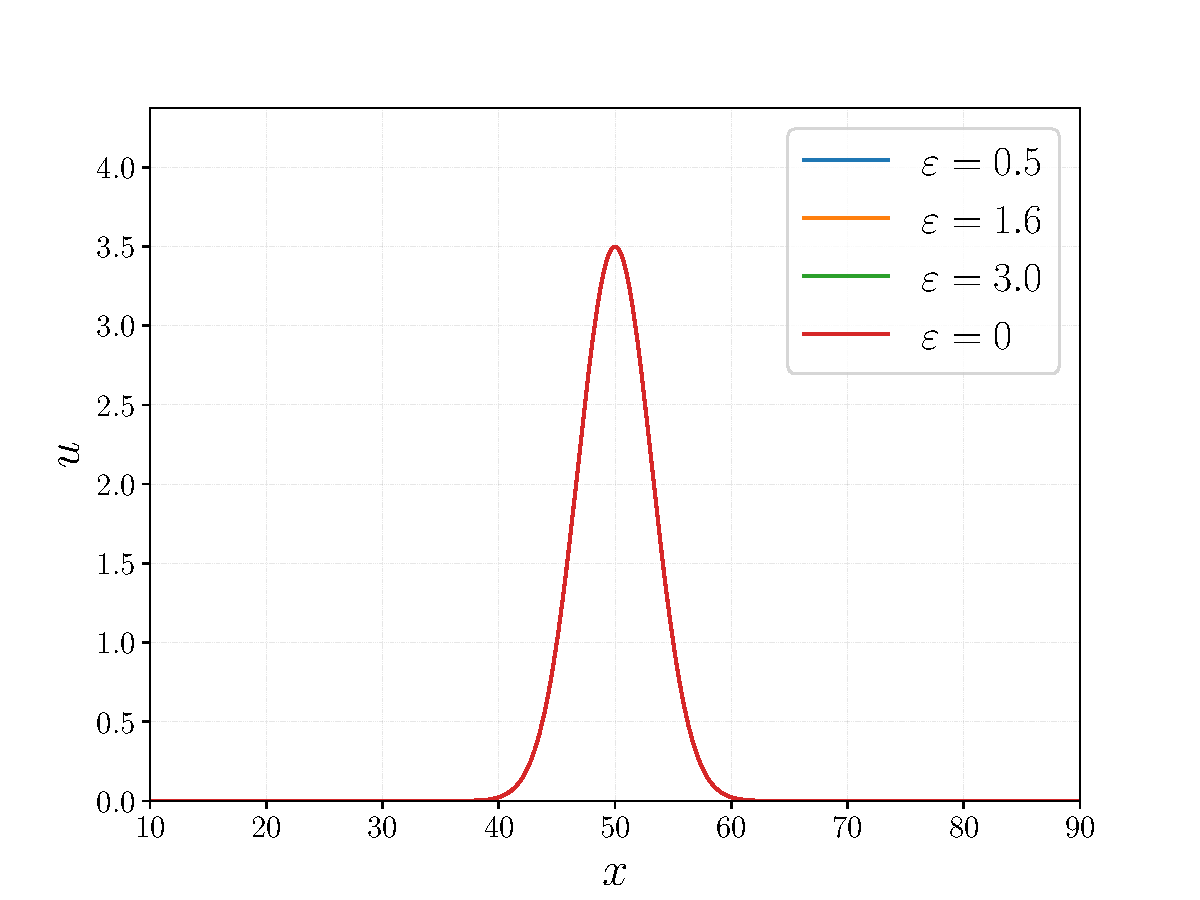
\includegraphics[width=\linewidth]{../some_plots/burgers-viscosas/graficas/viscosidades-1.pdf}
%		\caption{.}
		\label{fig:viscosas1}
	\end{subfigure}%
	\begin{subfigure}{0.5\textwidth}
		\centering
		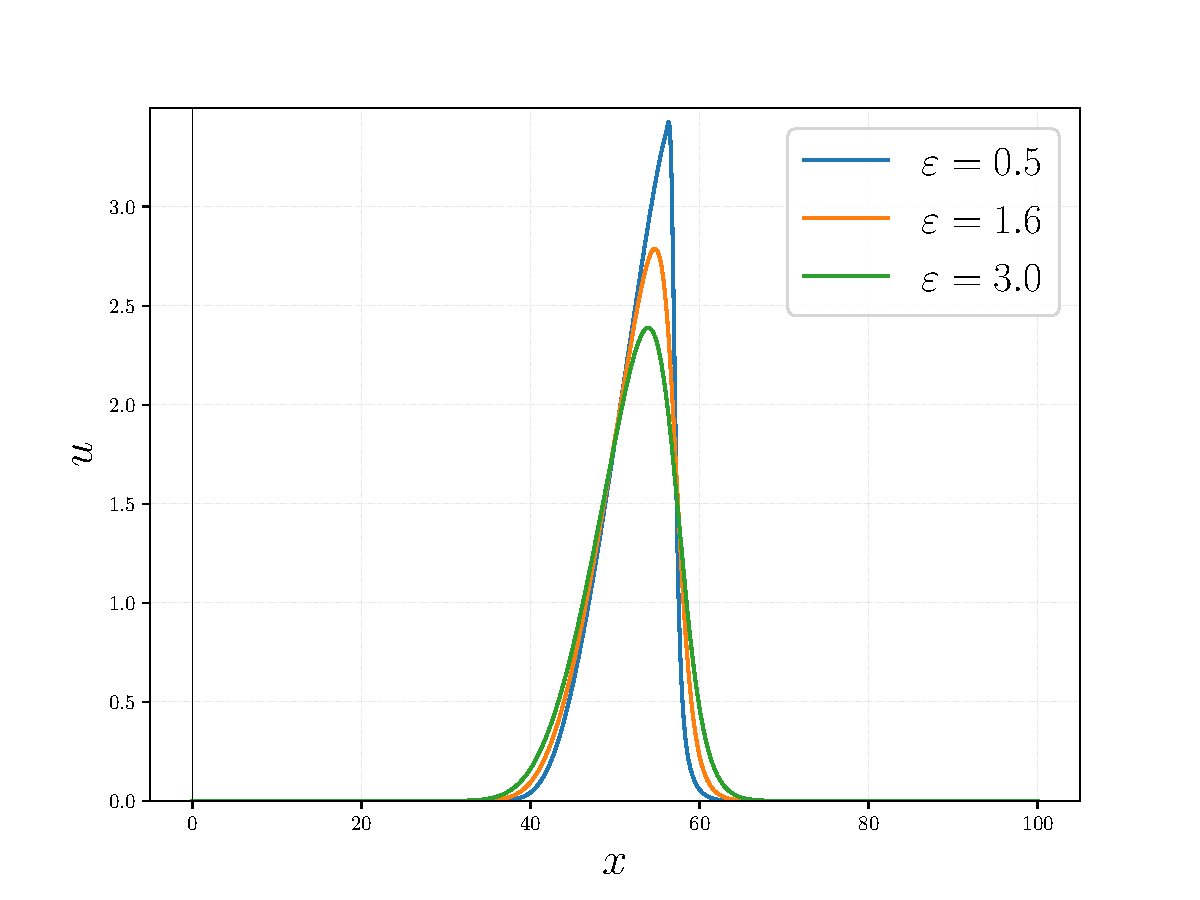
\includegraphics[width=\linewidth]{../some_plots/burgers-viscosas/graficas/viscosidades-100.pdf}
%		\caption{.}
		\label{fig:viscosas2}
	\end{subfigure}
	\begin{subfigure}{0.5\textwidth}
		\centering
		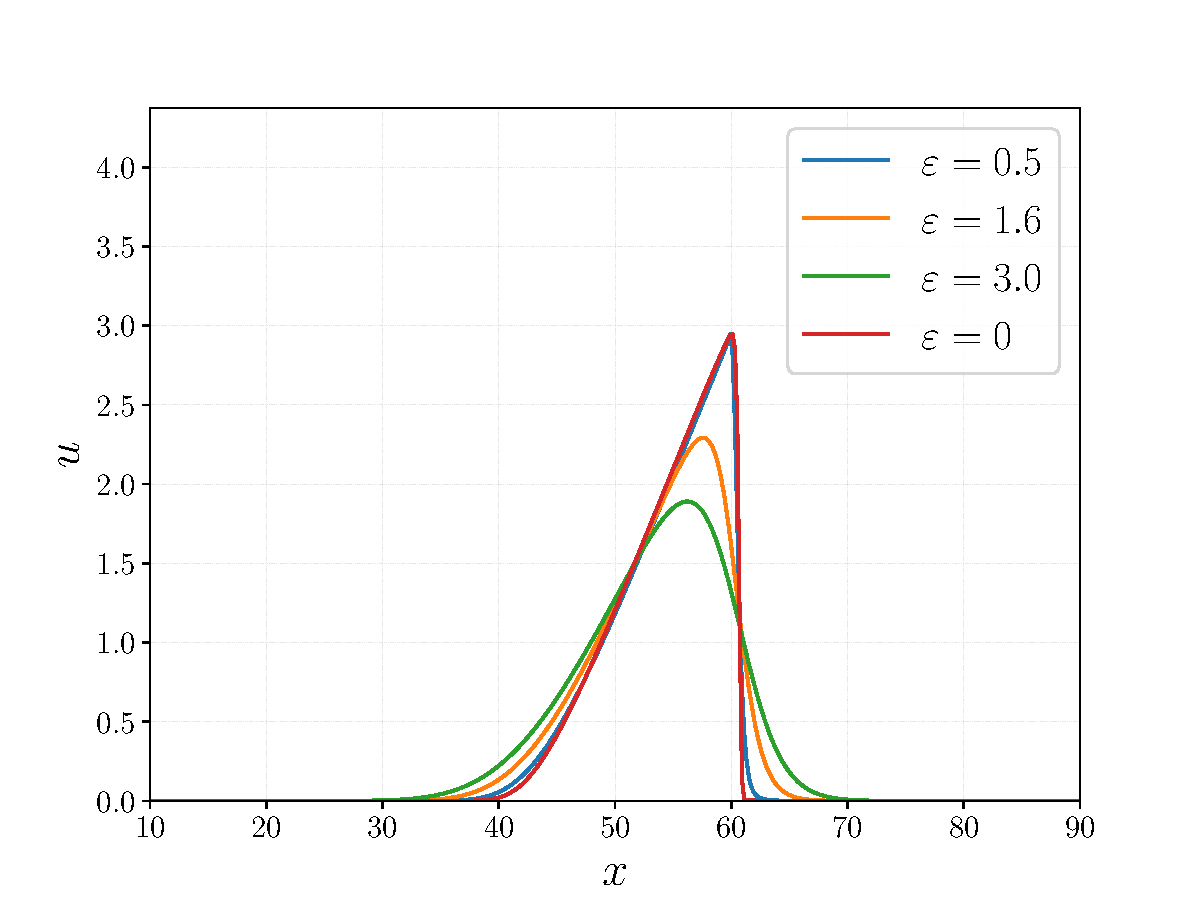
\includegraphics[width=\linewidth]{../some_plots/burgers-viscosas/graficas/viscosidades-200.pdf}
%		\caption{.}
		\label{fig:viscosas3}
	\end{subfigure}
	\begin{subfigure}{0.5\textwidth}
		\centering
		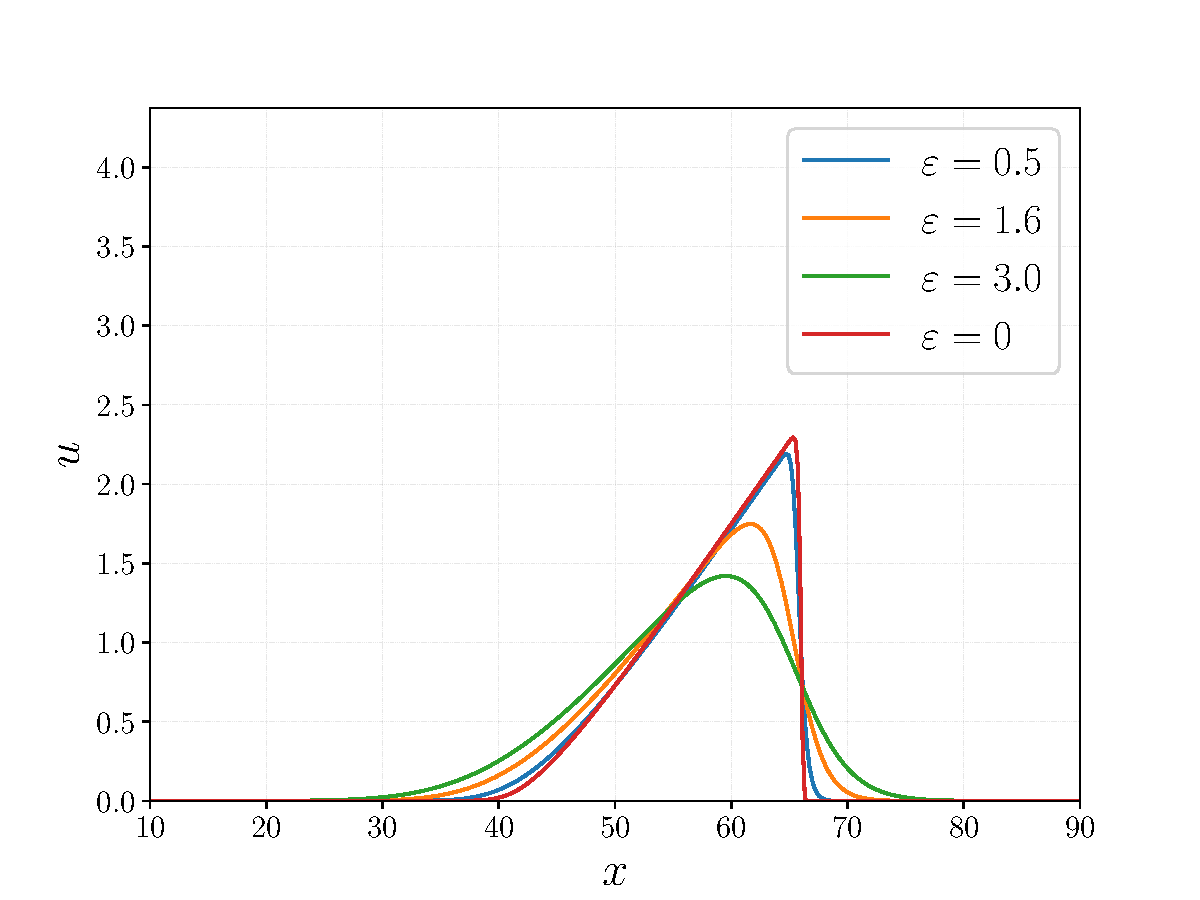
\includegraphics[width=\linewidth]{../some_plots/burgers-viscosas/graficas/viscosidades-400.pdf}
%		\caption{.}
		\label{fig:viscosas4}
	\end{subfigure}
	\caption{Gráficas de las soluciones numéricas, en distintos instantes de tiempo, de la ecuación de Burgers viscosa para distintos valores de coeficiente de viscosidad cinemática ($\varepsilon$), incluyendo el caso donde no hay viscosidad (en rojo). \textbf{Fuente:} elaboración propia.}
	\label{fig:viscosas}
\end{figure}

\section{Problema de Riemann}
Como se ha mostrado, las soluciones a las ecuaciones de conservación admiten soluciones débiles que pueden presentar discontinuidades tanto en la condición inicial como en la evolución temporal de las mismas. Por esta razón, es natural estudiar sistemas hiperbólicos con condiciones iniciales discontinuas, este problema es conocido como \textbf{problema de Riemann}. En el caso escalar, el problema de Riemann para una ecuación de conservación de la forma $u_t + f(u)_x = 0$ corresponde a la siguiente condición inicial
\begin{equation}
	u(x,0) = 
	\begin{cases}
		u_L & \text{si } x < 0 \\
		u_R & \text{si } x \geq 0,
		\label{eq:riemannLR}
	\end{cases}
\end{equation}
en donde la solución es determinada por la relación entre $u_L$ y $u_R$ \cite{Leveque}.
\subsection{Solución al problema de Riemann para la ecuación de Burgers}
Para encontrar la solución al problema de Riemann de la ecuación de Burgers es necesario considerar dos casos.
\subsubsection{Caso $u_L > u_R$:}
La función
\begin{equation}
	u(x,t) = 
	\begin{cases}
		u_L, & \hspace{3mm} x < st \\
		u_R, & \hspace{3mm} x > st,		
	\end{cases}\label{eq:solriemannLR}
\end{equation}
conocida como \textbf{onda de choque}, representa una discontinuidad trasladándose a través del eje $x$ con una velocidad $s$. Esta última es una solución débil de la ecuación de Burgers, para la condición inicial (\ref{eq:riemannLR}), si se cumple la condición general de  \textbf{Rankine - Hugoniot} \cite{Cameron}, que se define como:
\begin{equation}
	f(u_L) - f(u_R) = s(u_L - u_R),
	\label{eq:rankinehugo}
\end{equation}
donde $f(u) = \frac{1}{2} u^{2}$ \cite{Leveque}. A continuación se demuestra la expresión general de la condición Rankine - Hugoniot.\\

\textit{Prueba:} Sea $u$ una solución débil de la ecuación diferencial $u_t + f(u)_x = 0$, de la forma (\ref{eq:solriemannLR}). Sea $\mathcal{M} \gg st$. Aplicando la expresión (\ref{eq:continuidad-1-integral}) a $u$:
\begin{equation}
	\dv{t} \int_{-\mathcal{M}}^{\mathcal{M}}u(x,t)\dd{x} = f(u_L) - f(u_R).
	\label{eq:flux_diff}
\end{equation}
Integrando $u$ a partir de su definición (\ref{eq:solriemannLR}), se tiene
\begin{equation}
	\int_{-\mathcal{M}}^{\mathcal{M}}u(x,t)\dd{x} = (\mathcal{M} + st)u_L + (\mathcal{M} - st)u_R.
\end{equation}
Entonces, sustituyendo en (\ref{eq:flux_diff}),
\begin{equation}
	\dv{t}\left[(\mathcal{M} + st)u_L + (\mathcal{M} - st)u_R\right] = f(u_L) - f(u_R)
\end{equation}
\begin{equation}
	s(u_L - u_R) = f(u_L) - f(u_R),
\end{equation}
se obtiene la condición de salto de Rankine - Hugoniot \cite{Leveque}.

Por lo tanto, para el caso $u_L > u_R$, la solución de la ecuación de Burgers es una discontinuidad que se propaga con una velocidad constante $s = \frac{u_L + u_R}{2}$ \cite{Cameron}.

\begin{figure}[ht]
	\centering
	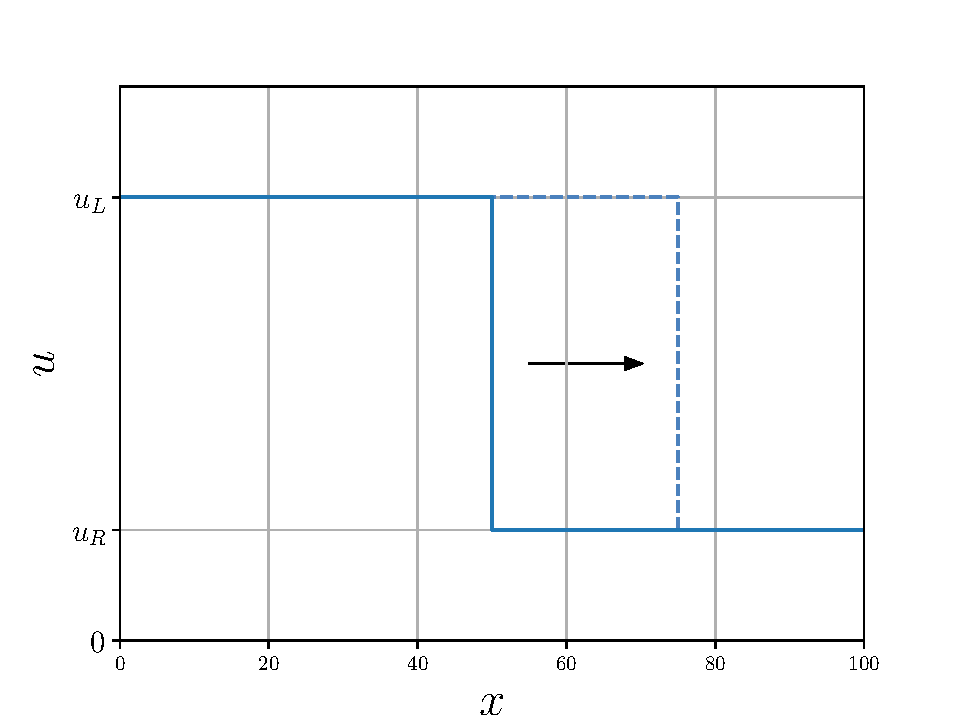
\includegraphics[width=0.8\linewidth]{../some_plots/cap1/graficas/riemannLR.pdf}
	\caption{Ejemplo gráfico de la solución de la ecuación de Burgers para el caso $u_L > u_R$. \textbf{Fuente: }elaboración propia, basada en el esquema obtenido de \cite{Leveque}.}
	\label{fig:solriemannLR}
\end{figure}

\subsubsection{Caso $u_L < u_R$:}
Hay múltiples soluciones débiles para este caso, por ejemplo, la solución (\ref{eq:solriemannLR}) \cite{Cameron} \cite{Leveque}. Sin embargo, esta no es la solución que corresponde a la solución con viscosidad disipiada \cite{Cameron}. La solución
\begin{equation}
	u(x,t) = 
	\begin{cases}
		u_L, & \hspace{3mm} x < u_{L}t \\
		x/t, & \hspace{3mm} u_{L}t \leq x \leq u_{R}t \\
		u_R, & \hspace{3mm} x > u_{R}t,		
	\end{cases}\label{eq:solriemannRL}
\end{equation}
es la solución correspondiente a la viscosidad disipada y es conocida como \textbf{onda de rarefacción} \cite{Leveque}. Resulta ser poco práctico tener que recurrir frecuentemente a la solución de viscosidad disipada para encontrar la solución a cualquier caso del problema de Riemann, por lo que en su lugar se suelen imponer condiciones conocidas como \textbf{condiciones de entropía} que son equivalentes a exigir que la solución sea consistente con el formalismo de viscosidad disipada \cite{Leveque}.

\begin{figure}[ht]
	\begin{subfigure}{0.5\textwidth}
		\centering
		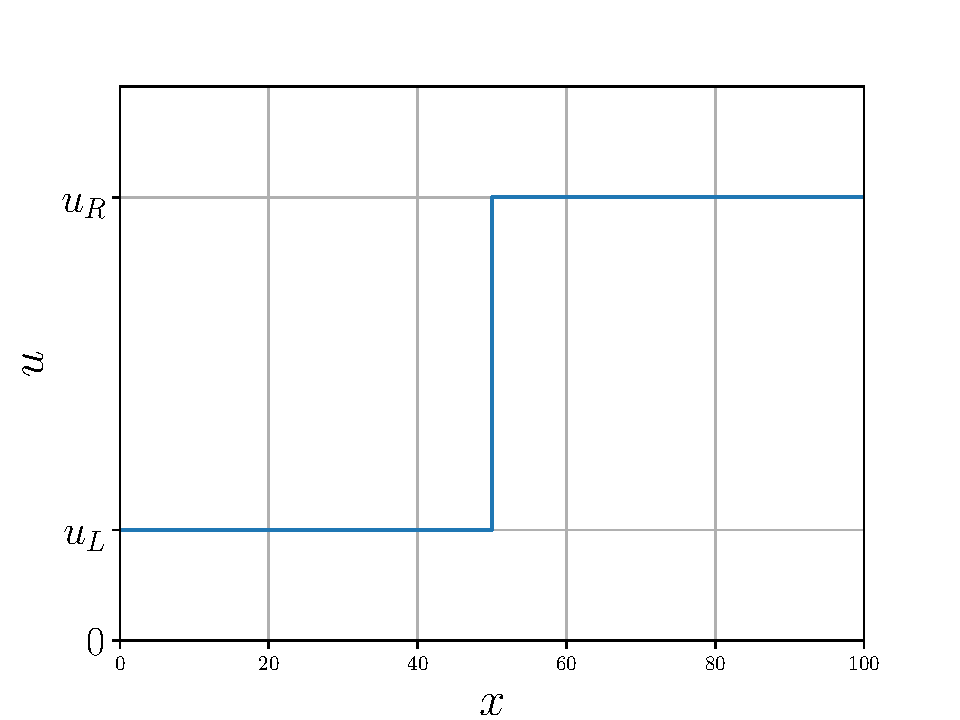
\includegraphics[width=\linewidth]{../some_plots/cap1/graficas/riemannRL-0.pdf}
		%		\caption{.}
%		\label{fig:rarefaccion}
	\end{subfigure}%
	\begin{subfigure}{0.5\textwidth}
		\centering
		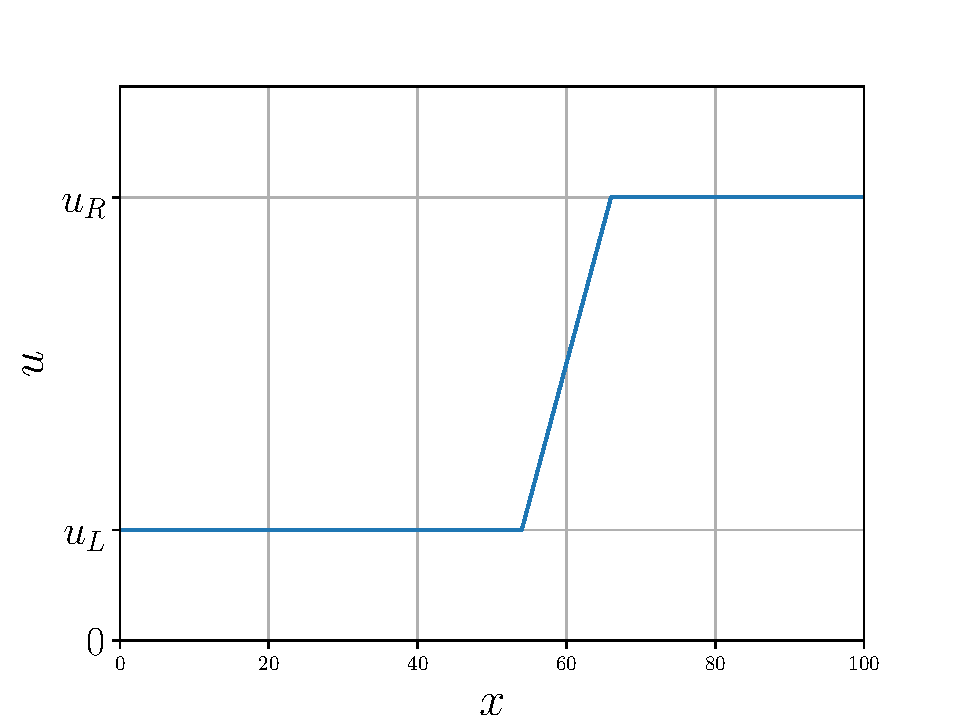
\includegraphics[width=\linewidth]{../some_plots/cap1/graficas/riemannRL-0.4.pdf}
		%		\caption{.}
%		\label{fig:viscosas2}
	\end{subfigure}
	\begin{subfigure}{0.5\textwidth}
		\centering
		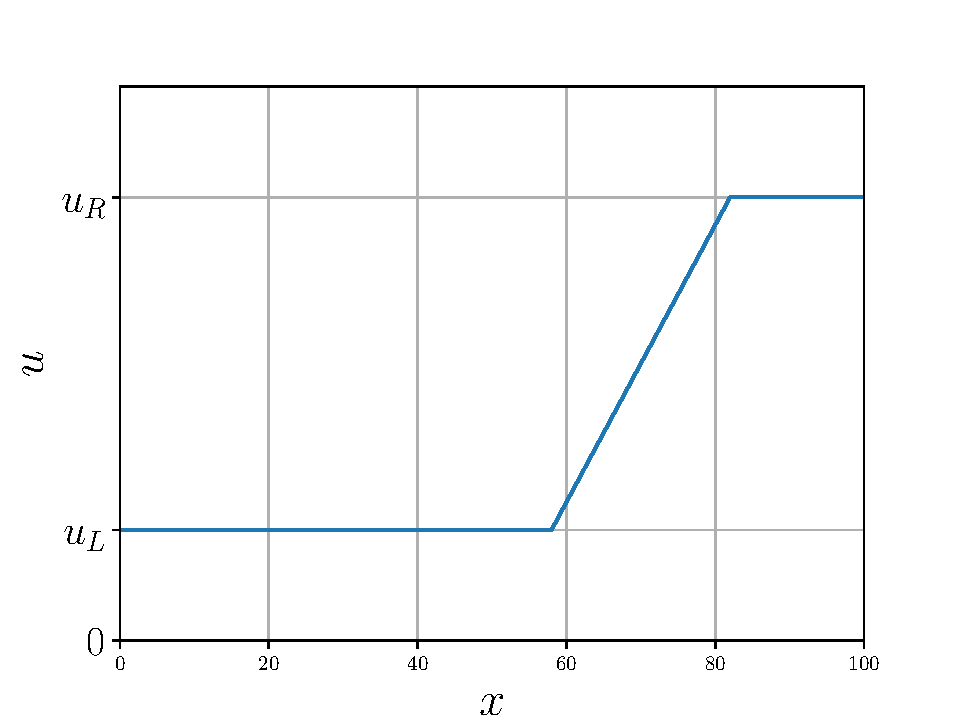
\includegraphics[width=\linewidth]{../some_plots/cap1/graficas/riemannRL-0.8.pdf}
		%		\caption{.}
%		\label{fig:viscosas3}
	\end{subfigure}
	\begin{subfigure}{0.5\textwidth}
		\centering
		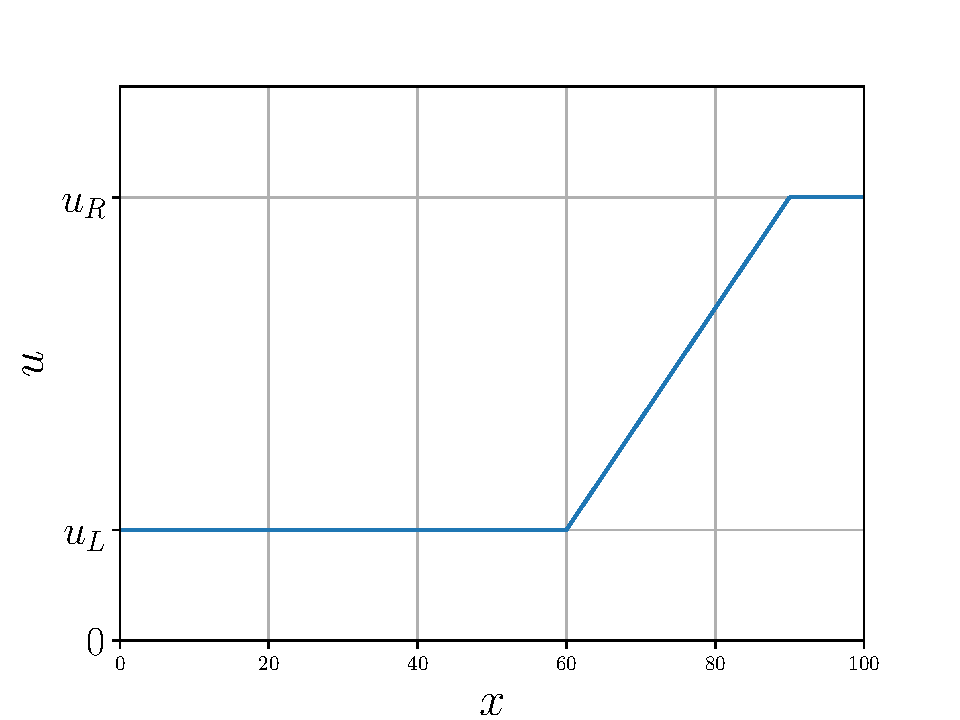
\includegraphics[width=\linewidth]{../some_plots/cap1/graficas/riemannRL-1.pdf}
		%		\caption{.}
%		\label{fig:viscosas4}
	\end{subfigure}
	\caption{Gráficas de las soluciones, en distintos instantes de tiempo, de la ecuación de Burgers para el caso $u_L < u_R$ del problema de Riemann \textbf{Fuente:} elaboración propia.}
	\label{fig:rarefaccion}
\end{figure}


\par}               % termina interlineado 1 1/2

\end{document}
